%%============================================================================
%% thesis.tex  --  Adelaide Punt, DPhil thesis (body)
%%
%% Title: Noise and Uncertainty in Molecular Property Prediction:
%%        Robust Models and Adaptive Representations
%%============================================================================

% TODO: REVIEW MODIFICATION (30 Sep) -- tables that ran into the margin now fit: every tabular in a table float is
% wrapped in adjustbox (shrinks only if too wide), the widest headers are split over two lines, and the
% longtable column widths were cut so they fit the 15cm text width.
% TODO: REVIEW MODIFICATION -- every \caption now has a one-line short form in [ ]. Only the short
% form appears in the List of Figures and List of Tables, as in Dablander's thesis.

\chapter{Introduction}\label{chap:intro}
% [notes moved to thesis_notes_moved.md]

% TODO: review, needs manual review
New avenues in the drug discovery pipeline have opened up thanks to advances in large dataset collection, analysis, and computation. Therapeutic targets are identified, potential drug candidates are screened and optimized, and the most promising of these go on to pre-clinical and clinical trials \citep{Lill2007}. There are various methods by which potential drug candidates can be screened. Virtual screening allows for the rapid and large-scale analysis of libraries of compounds, and is a particularly useful approach used to speed up the drug discovery process \citep{Neves2018}. One standard screening method is the prediction of bioactivities and pharmacological properties of such candidates. There is a long history of using quantitative structure--activity relationship (QSAR) models to make these predictions, to act as a filter for compounds with undesirable properties, and thus reduce the time and cost associated with experimental screening \citep{Sabando2021}. QSAR models learn the relationship between a molecule's features, as encoded by a molecular representation, and a property of interest \citep{Sabando2021}. A QSAR model typically consists of a molecular representation paired with a machine learning (ML) model. An ideal molecular representation will allow a model to learn only the relevant information about each molecule with respect to the target property. Representations are either `static' hand-crafted descriptors or circular fingerprints that encode predefined structural and physicochemical features \citep{rogers2010, David2020, sns, avalon}; or learned representations, where the encoding is derived from a predictive model, often taken from the activations of the final layer of a neural network, or a latent space embedding \citep{Sabando2021, kishimoto2023}. 

QSAR models are, of course, sensitive to the quality of the input data on which they are trained. Experimental noise can arise from measurement errors, variability under experimental conditions, varying provenance of the data, and intrinsic biological and chemical variability. Even the very measures of model performance may be flawed if test and validation sets are laden with noise. \citet{Kolmar2021} show that the variance associated with experimental data can contribute more to prediction error than the model’s own error. There is also a limit to how much noise the model can tolerate; \citet{jorner2021} found that once the model error approaches the magnitude of the experimental measurement error on labels, adding more training data yields diminishing returns in predictive performance. In the context of activity prediction, the inherent variability within experimental setups and assays, batch effects, measurement errors, and biological variability introduce additional layers of complexity \citep{Kolmar2021, Fourches2010}. All of this increases the likelihood of encountering noise in the data \citep{Fang2022}. Even the molecular representations in the training data themselves may be incorrect or misleading \citep{Walters2023}, and chemical datasets contain too few repeat measurements of each compound to characterize the distribution the label is drawn from. Thus, models treat a single label as the population mean \citep{Kolmar2021}. Repeat measurements of the same compound-target pair disagree by about $0.68$ log units for pIC$_{50}$, and by about $0.54$ log units for p$K_i$ \citep{Kalliokoski2013, Kramer2012}. Measurements from a single assay lower the mean disagreement from $0.50$ to $0.27$ log units \citep{landrum2024}.
% TODO: the 0.50 baseline sits beside 0.68 (pIC50) and 0.54 (pKi) without saying which comparison it comes from; check landrum2024 and say what 0.50 is measured over.  

% TODO: REVIEW MODIFICATION -- Chapter 1 restructured to match Dablander: prose, then the Outline as Section 1.1.
% What changed, in order:
% - Intro paragraphs 1-2 (QSAR, noise) unchanged.
% - Your paragraph 3 ("This thesis addresses...") and old Section 1.1 ("The questions this thesis asks") are merged into
%   the next paragraph. Your sentence "As we will show, both model and representation choice dominate predictive
%   performance on clean data, however, this relationship inverts..." is cut: it is a Chapter 3 finding, and the
%   Outline states Chapter 3's findings.
% - Your paragraph 4 ("Building on these findings, I began...") is replaced by the two paragraphs from old Section 1.2
%   on the exploratory study and on the distance hypothesis. Your original is kept commented out below.
% - Old Section 1.2's first paragraph (the Chapter 3 variance shares and uncertainty findings) is cut. Kept commented out below.
% - Old Section 1.2's heading is gone. Its notes block moved to thesis_notes_moved.md.
% - The label sec:intro:questions now sits on the questions paragraph; references to it now say Chapter 1.
% - The funding paragraph from "Collaborations and funding" moved to the Acknowledgements in main.tex.

% [TRIM3 2026-09-30] simplified
% CODE INPUT: merged from your paragraph 3 and old Section 1.1, in your wording
% [RESTORE 2026-09-30] Ch1-1 Ch1-2 Ch1-3 Ch1-4
% TODO: review, needs manual review
This thesis addresses the challenge of conducting molecular property prediction when the underlying experimental data contain noisy labels. Most work on noise in QSAR modeling assumes Gaussian label noise and evaluates either representations or model architectures in isolation. \citet{Cortes2015} examined 12 algorithms across multiple noise levels but used fixed representations, and studies that compare representations typically use clean data. No work has systematically compared the relative importance of representation versus architecture choice for noise robustness, asked whether probabilistic methods justify their computational overhead under noise, or tested whether findings generalize across corruption patterns and property types. The first half of this thesis therefore asks four questions.\label{sec:intro:questions} First, how much of the variance in predictive performance do representation and model architecture each explain, and does that division change for the performance retained under increasing label noise? Second, what does the choice of model provide under label noise, and how do deterministic and probabilistic models compare? Third, does the type of label noise matter, or only its quantity? To answer this, we generate and add label noise in several ways, both to clean data and to data with inherent experimental noise. Fourth, what is the impact of artificial label noise on a model's uncertainty estimates? In particular, does the estimated uncertainty rise with increasing label noise, and can it identify which labels are corrupted? Together, these questions aim to identify what, if anything, makes a QSAR model robust to noise. To answer them we introduce NoiseInject, an open-source Python package for benchmarking noise robustness and uncertainty quantification (Section~\ref{sec:noiseinject_pkg}).

% [TRIM3 2026-09-30] simplified
% [TRIM2 2026-09-30] added one sentence on the exploratory LNL study result
% TODO: review, needs manual review
% CODE INPUT: moved from old Section 1.2
Learning with noisy labels (LNL) covers methods for training models when some labels are wrong; noise mitigation, which removes, reweights or corrects labels, is one part of it (Section~\ref{sec:lnl_background}). In an exploratory study carried out earlier in this project, twelve LNL methods were adapted to regression and tested in 221 configurations on the QM9 HOMO--LUMO gap with Gaussian noise, and the 20 configurations that retained the least $R^2$ under noise all used a distance between molecules (Section~\ref{sec:lnl_motivation}).
% - Twelve LNL methods were adapted to regression and tested in 221 configurations on the QM9 HOMO-LUMO gap with Gaussian noise.
% - Several variants judged a label by its neighbors' labels, using a distance between molecules.
% - All 20 configurations with the lowest retention of R^2 under noise used such a distance.
% - This held for each distance tried: Tanimoto on ECFP4, Euclidean on physicochemical descriptors, and Mahalanobis.
% - The methods that held up estimated noise from the model's own loss or uncertainty, not from neighbors.
% - One dataset and one noise type: state it as the motivation, not a general result.
%
% Paragraph 3: why the distance failed, and the step to the hybrid (Chapters~\ref{chap:flaws}, \ref{chap:method} and \ref{chap:similarity})
% - Hypothesis: on a given dataset, most features of a general-purpose representation do not vary or do not relate to the property.
% - Every such feature adds a term to the distance, so irrelevant features dominate it. The growth is linear in the number of features, not exponential.
% - Chapter~\ref{chap:flaws} measures this on base representations and on distances.
% - The proposed fix: select a fixed number of task-relevant features from several representations, and compute distances in that compact space.
% - A first version showed that these selected feature sets also work as ordinary model inputs, with no distance involved.
% - That turned the question into how to choose the features, which is Chapter~\ref{chap:method}.
% - Chapter~\ref{chap:similarity} then returns to distances, noise detection and LNL, including noise mitigation, with the hybrid as the feature space.
% ---- END NOTES ----

% [TRIM3 2026-09-30] simplified
% [TRIM 2026-09-30] shortened
% CODE INPUT: moved from old Section 1.2
% TODO: review, needs manual review
We hypothesized that the fault lay in this distance. On a given dataset, most features of a general-purpose representation either do not vary or do not relate to the property, yet each adds a term to the distance, so together they dominate it (Chapter~\ref{chap:flaws}). We propose instead to compute distances over a hybrid representation: a fixed number of task-relevant features selected from several representations. A first version showed that the selected features also work as ordinary model inputs, so the question became how to choose them (Chapter~\ref{chap:method}).

% [TRIM3 2026-09-30] simplified
% TODO: review, needs manual review
The second half asks whether the representation itself can be adapted to the task:\label{sec:intro:hybrid_questions}
% DECISION FOR ADELAIDE: these five questions do not match the three research questions set out in the Chapter 6 introduction, and questions 2 and 5 have no reported result yet in Chapters 5 or 6 (Chapter 7 answers neither). Align this list with Chapters 5 and 6 once the full runs are in.
\begin{enumerate}
    \item How can the best set of features be selected for a given prediction task?
    \item Do hybrid representations retain more of their predictive performance under label noise than their base representations?
    \item Do the features selected for a hybrid representation help stabilize distance-based noise mitigation?
    \item Does weighting features by their importance improve the construction of hybrid representations, model training and noise mitigation?
    \item When sample removal is suboptimal, can sample weighting or label smoothing handle Gaussian label noise better?
\end{enumerate}

% ---- REMOVED (kept for your review; delete once checked) ----
% This thesis addresses the challenge of conducting molecular property prediction when the underlying experimental data contain noisy labels. The first research question is which combinations of molecular representations and predictive model architectures maintain predictive performance under label corruption, and whether probabilistic methods that estimate uncertainty justify their additional complexity. As we will show, both model and representation choice dominate predictive performance on clean data, however, this relationship inverts under label corruption as predictive architecture becomes the primary factor in determining noise robustness.  Most existing work on noise in QSAR modelings assumes that label noise can be modeled as random error drawn from a Gaussian distribution, and they evaluate either molecular representations or predictive model architectures in isolation. \citet{Cortes2015} examined 12 algorithms across multiple noise levels but used fixed representations. Studies that compare representations are typically done on clean data. No work has systematically compared the relative importance of representation versus architecture choice for noise robustness, assessed whether probabilistic methods justify their computational overhead in noisy settings, or tested whether findings generalize across different corruption patterns and molecular property types.
% 
% Building on these findings, I began exploring techniques involving learning with noisy labels and noise mitigation. Many of these methods incorporate measures of molecular similarity, relying on the assumption that molecules which are similar in structure share similar properties \citep{LopezPerez2024}. However, all of the methods that used simiarity estimates failed, even when I tried varying the molecular representations and vector operations from the standard ECFP4 and Tanimoto coefficient. I hypothesized that to generate accurate similarity estimates, you need a specialized molecular representation who's features relate directly to similarity in that molecular domain. This brings me to my next research question, how do you select the best set of features for a given prediction task? I will outline how I developed an adaptive feature selection methodology that takes in a set of molecular representations, identifies each representation's most important features, and combines a select set of those top features into a new hybrid representation. I will then demonstrate how it improve performance across a range of predictive tasks beyond the small molecule space, and how it can be applied to the context of similarity estimation and downstream noise mitigation methods. 
% 
% The first half of this thesis addresses four questions about the behavior of QSAR models under label noise. First, how does the choice of molecular representation and model architecture explain the variance in predictive performance, and does that division change when you instead consider how much performance a QSAR model is able to retain under increasing label noise? Second, what does the choice of model provide with label noise? Within this question we compare the effects of deterministic and probabilistic modeling. Third, does the type of label noise matter, or just the quantity of it? We explore different techniques of generating and adding label noise to both clean data, as well as data with inherent experimental noise. Fourth, what is the impact of artificial label noise on a model's uncertainty estimation? Does the estimated uncertainty rise with increased label noise and can these uncertainty values point to which labels are corrupted? Together, these questions aim to identify what, if anything, makes a QSAR model robust to noise. Finally, we introduce NoiseInject, an open-source Python package for benchmarking noise robustness and uncertainty quantification in machine learning models.
% 
% % CODE INPUT
% % TODO: Ch3 update -- re-check the Chapter 3 results quoted in this paragraph against the updated chapter.
% The first half of this thesis measures how QSAR models behave as label noise rises (Chapter~\ref{chap:robustness}). We define robustness as the normalized area under the curve of $R^2$ retained as noise increases. Under Gaussian noise on QM9, model architecture explains 49.5\% of the variance in robustness, and representation explains 9.2\%. For $R^2$ at noise level 1.0, where the noise has the same spread as the clean training labels, the two shares are comparable: 29.1\% for architecture and 26.6\% for representation. These shares are measured under noise. \textbf{[RESULT NEEDED: the same variance split on $R^2$ before any noise is added.]} Systematic noise did the most damage: noise shared within a scaffold family, and labels clipped at an assay limit. The shape of the noise distribution barely mattered. Under Gaussian noise on QM9, mean predicted uncertainty rose with noise for every probabilistic model and representation. Per-molecule uncertainty, however, did not reliably pick out which labels were corrupted (Section~\ref{sec:uq}). NGBoost and the Gaussian process fit a separate scale for each molecule. They gave the strongest per-molecule correlation between predicted uncertainty and injected noise. Under censoring, models were most confident on the labels that had been clipped. Uncertainty alone therefore cannot tell us which labels to fix. This led us to methods that judge each label in another way.
% ---- END REMOVED ----


\section{Outline of the Thesis and Contributions}

% ---- NOTES: Outline of the thesis and contributions ----
% Takeaway: one short paragraph per chapter: what it does, what it found (Chapters 3 and 4) or will test (Chapters 5 and 6), and where it is published or planned.
%
% Paragraph 1: Chapter 2 (Background)
% - Introduces, once, what the later chapters rely on: molecular representations, model families, molecular similarity and activity cliffs, noise in molecular data, and the evaluation protocol.
% - Defines the seven noise conditions used in Chapter 3.
% - Ends by introducing NoiseInject, the open-source benchmarking framework released with this work.
%
% Paragraph 2: Chapter 3 (Noise robustness across molecular representations and model architectures)
% - Adapted from the paper "NoiseInject: A Benchmarking Framework to Study Noise Robustness in QSAR Models" by Punt, Hanser, Werner and Morris, in preparation for the Journal of Cheminformatics. Say this in the paragraph.
% - Main task: the HOMO-LUMO gap on QM9. Its labels are computed, so they carry negligible measurement noise.
% - Repeated on three assay datasets with experimental labels: LogD, Caco-2 and hERG Ki.
% - Splits the variance in performance, and in how much performance is retained under noise, between representation and model architecture.
% - Compares seven noise conditions at a matched amount of noise.
% - Compares each model with its probabilistic counterpart, and asks what label noise does to predicted uncertainty.
% - Findings in words only, no numbers:
% - Model architecture matters more than representation for noise robustness. For R^2 under noise, the two matter about equally.
% - The shape of the noise distribution makes little difference. Noise shared within a scaffold family, and labels clipped at an assay limit (censoring), do the most damage.
% - NGBoost and random forests were the most robust models on QM9. Random forests were the most consistent across all four datasets.
% - Predicted uncertainty rises with noise on average, but does not pick out which labels were corrupted.
%
% Paragraph 3: Chapter 4 (The flaws of the similarity assumption)
% - A motivation chapter. It introduces no method, and its measurements are smaller than Chapter 3's.
% - First argument: on a given dataset, standard representations carry many features that do not vary, and some map different molecules to the same vector.
% - Second argument: similarity computed over those representations inherits both problems.
% - Third argument: methods that rely on that similarity fail as a result.
% - These include cleaning labels by comparing each molecule's label with its nearest neighbors' labels, a noise mitigation method tested in the exploratory study of learning with noisy labels. Say plainly that this study comes from the confirmation report.
% - Ends by stating what a representation would need to fix this. That is what Chapter 5 builds.
%
% Paragraph 4: Chapter 5 (Building adaptive hybrid representations)
% - Planned as the first of two method papers. Intended for submission; venue to be confirmed.
% - The method: from several base representations, it selects each one's most important features for the task.
% - It splits a fixed budget of features between the representations and combines the selected features into one representation.
% - Also describes the datasets and the experimental setup.
% - Will test when the hybrid helps, against the best single representation and against an ensemble of one model per representation.
% - Will test why it helps, against PCA, mRMR, recursive feature elimination and random features at the same number of features.
% - Will test whether the selected features can be read against the chemistry, and how stable the selection is across folds.
% - Will test whether search settings found on one dataset carry to another.
% - Will test whether it extends beyond small molecules: antibodies in most depth, and reactions, nucleotide sequences and cancer genomics as proofs of concept.
% - Will test whether it extends to data held at separate sites that cannot be pooled.
% - Result needed: one sentence of findings for Chapter 5.
%
% Paragraph 5: Chapter 6 (Hybrid representations for similarity and label noise)
% - Planned as the second method paper. Intended for submission; venue to be confirmed.
% - Returns to the failures in Chapter 4 and asks whether a hybrid representation repairs them.
% - Similarity: hybrids selected for predicting each molecule's activity from its five nearest neighbors, compared with standard representations.
% - Noise detection and estimation: whether neighbors in a hybrid pick out corrupted labels better than neighbors in a standard representation.
% - Learning with noisy labels, including noise mitigation, one noise type at a time.
% - Result needed: one sentence of findings for Chapter 6.
%
% Paragraph 6: Chapter 7 (Discussion and future directions)
% - Summarizes each chapter.
% - Closing argument: model the noise before choosing a method. No single method fits every dataset, and simple methods are often as good.
% - Then limitations and future directions.
%
% Paragraph 7: Contributions (short: publications and software)
% - Publications: the Chapter 3 paper (in preparation) and the planned papers from Chapters 5 and 6. Point to the Research Papers list in the Summary of Research Contributions rather than repeating it.
% - Software: NoiseInject (open source), and the KIRBy software repository that implements the hybrid search and its experiments.
% - Repositories, licenses and data: point to Additional file~\ref{app:availability}.
% ---- END NOTES ----

% [TRIM3 2026-09-30] simplified
% CODE INPUT
% TODO: review, needs manual review
Chapter~\ref{chap:background} introduces molecular representations, model families, molecular similarity and activity cliffs, and the sources of noise in molecular data. It defines the seven noise conditions used in Chapter~\ref{chap:robustness} and the methods for LNL, and it closes with NoiseInject and the evaluation metrics.

% [TRIM3 2026-09-30] simplified
% CODE INPUT
% [TRIM4 2026-09-30] cut the sentence naming the most robust models; the Chapter 3 Conclusions carry it
% TODO: Ch3 update -- re-check the Chapter 3 results quoted in this paragraph against the updated chapter.
% (30 Sep: findings below rewritten to follow the new Chapter 3 Conclusions.)
% TODO: review, needs manual review
Chapter~\ref{chap:robustness} studies the noise robustness of QSAR models, mainly on the gap between the highest occupied and lowest unoccupied molecular orbitals (HOMO--LUMO gap) in QM9, whose computed labels carry negligible measurement noise, and on three assay datasets: LogD, Caco-2 and hERG $K_i$. It addresses the four questions above, comparing seven noise conditions, all but censoring at a matched amount of noise, and each model with its probabilistic counterpart. Model family explains the largest share of the variance in noise robustness, while representation explains at most 11.2\% of it and a larger share of the variance in predictive performance than of the variance in robustness. The shape of the noise distribution makes little difference, whereas an offset shared within each scaffold family and labels clipped at an assay limit (censoring), the two conditions in which the error is systematic, give the lowest robustness. On the assay datasets, turning a feed-forward network into a Bayesian one raised its robustness at a cost in predictive performance on clean labels. Mean predicted uncertainty rises with noise for almost every probabilistic model on QM9 and for most models on the assay datasets, but per-molecule uncertainty does not identify which labels were corrupted. The exception is censoring: the models are most confident on the clipped labels, so dividing each molecule's error by its uncertainty picks them out better than the error alone.

% [TRIM3 2026-09-30] simplified
% CODE INPUT
% [RESTORE 2026-09-30] Ch1-6
% TODO: review, needs manual review
Chapter~\ref{chap:flaws} motivates the later methods. It introduces no method of its own, and its measurements are on a smaller scale than those of Chapter~\ref{chap:robustness}. On a given dataset, standard representations carry many features that do not vary, and some map different molecules to the same vector. Similarity computed over these representations inherits both problems, and methods that rely on it fail as a result. These include a noise mitigation method, tested in the exploratory study, that cleans each label by comparing it with its nearest neighbors' labels. The chapter ends with what a representation would need to fix these problems, which Chapter~\ref{chap:method} builds.

% [TRIM3 2026-09-30] simplified
% [TRIM4 2026-09-30] planned comparisons cut to one sentence listing them
% CODE INPUT
% DECISION FOR ADELAIDE: Chapters 1 and 6 plan two method papers, but the Research Papers list in the Summary of Research Contributions gives one paper covering Chapters 5 and 6; make them agree.
% TODO: review, needs manual review
Chapter~\ref{chap:method}, planned as the first of two method papers, presents the adaptive hybrid representation. From each of several base representations, the method selects the features most important for the task, divides a fixed budget of features between them, and combines the selected features into one representation. The chapter also describes the datasets and setup. It will compare the hybrid with the best single representation, an ensemble of one model per representation, principal component analysis, minimum-redundancy maximum-relevance selection, recursive feature elimination and random features of the same size. It will also test whether the selected features are interpretable and stable, whether search settings transfer between datasets, and whether the method extends to other domains and to data held at separate sites. Its results so far are preliminary. In local runs on hERG $K_i$ with one default configuration, the hybrid had a lower root mean squared error than the best single representation with a support vector machine and with LightGBM on all three folds, and was level with it for random forest. At the same number of features it was ahead of principal component analysis and random features, but recursive feature elimination was ahead of it.
% TODO: replace the preliminary sentence above with the finding from the full runs for Chapter 5.

% [TRIM3 2026-09-30] simplified
% CODE INPUT
% [RESTORE 2026-09-30] Ch1-7
% TODO: review, needs manual review
Chapter~\ref{chap:similarity}, planned as the second method paper, asks whether a hybrid representation repairs the failures described in Chapter~\ref{chap:flaws}. It compares standard and hybrid representations selected for predicting each molecule's activity from its five nearest neighbors, asks whether neighbors in a hybrid representation identify corrupted labels better than neighbors in a standard one, and tests LNL methods, including noise mitigation, one noise type at a time. Its results are also preliminary. On hERG $K_i$, predicting each molecule's activity from its five nearest neighbors was more accurate in a hybrid than in the best single representation, and, on ECFP4, correcting labels clipped at a limit by one shared amount recovered more than half of the lost performance, whereas deleting the clipped molecules gave a higher error than keeping them. Under Gaussian noise on nanobody thermostability, every one of twelve LNL methods scored higher on the hybrid than any of them did on one-hot, the weakest input.
% TODO: replace the preliminary sentences above with the findings from the full runs for Chapter 6.

% [TRIM3 2026-09-30] simplified
% CODE INPUT
% TODO: review, needs manual review
Chapter~\ref{chap:discussion} summarizes each chapter and argues that the noise in a dataset should be modeled before a method is chosen, since no single method fits every dataset and simple methods are often as good as complex ones. It then gives limitations, future directions and conclusions. % TODO: REVIEW MODIFICATION -- Chapter 7 now ends with Conclusions

% [TRIM3 2026-09-30] simplified
% CODE INPUT
% TODO: review, needs manual review
The software contributions are NoiseInject and the KIRBy repository, which implements the search for hybrid representations and the experiments (Additional file~\ref{app:availability}).


% TODO: REVIEW MODIFICATION -- was "Collaborations and funding"; funding moved to the Acknowledgements.
\section{Collaborations}
% [notes moved to thesis_notes_moved.md]

% CODE INPUT
% TODO: REVIEW MODIFICATION -- funding paragraph moved to the Acknowledgements (main.tex).
% This DPhil was funded by the University of Oxford's UK EPSRC Centre for Doctoral Training in Sustainable Approaches to Biomedical Science: Responsible and Reproducible Research, grant EP/S024093/1. It was also supported by Lhasa Limited, a not-for-profit organization.

% [TRIM3 2026-09-30] simplified
% [TRIM2 2026-09-30] dropped the hERG molecule counts
% CODE INPUT
% TODO: review, needs manual review
This work was supervised by Garrett Morris and co-supervised by Thierry Hanser and St\'ephane Werner at Lhasa Limited, which runs the federated learning platform Effiris \citep{Bassani2023}. Lhasa also supplied the hERG data used in Chapters~\ref{chap:flaws} and~\ref{chap:method}; in Chapter~\ref{chap:method}, two of its sets and the public ChEMBL hERG $K_i$ set are treated as data held at separate sites, as in federated learning \citep{Bassani2023, Hanser2023}.

% [TRIM3 2026-09-30] simplified
% CODE INPUT
% TODO: review, needs manual review
The Oxford Protein Informatics Group (OPIG) pointed us to the antibody and protein datasets used in Chapters~\ref{chap:method} and~\ref{chap:similarity}; all datasets are listed in Additional file~\ref{app:datasets}. The collaboration also produced five posts on OPIG's blog, Blopig, listed under Blog Posts in the Summary of Research Contributions.

% [TRIM2 2026-09-30] "my own work" changed to "the author's own work"
% CODE INPUT
% TODO: review, needs manual review
The adaptive hybrid representation, its software and the experiments in Chapters~\ref{chap:flaws} to~\ref{chap:similarity} are the author's own work.



\pagebreak
% TODO: REVIEW MODIFICATION -- chapter title was "Background". Pick your own title; it should name what the chapter covers.
\chapter{Molecular Representations, Models and Label Noise}\label{chap:background}\label{sec2}
% ---- TAKEAWAYS ----
% - A representation turns a molecule into a fixed-length vector of features. Each family captures different information and has its own weakness, so no single one captures everything.
% - Model families differ in how far one wrong label spreads: a tree keeps it in one leaf, an ensemble dilutes it, a neural network can memorize it.
% - Similarity only exists relative to a representation and a coefficient. Activity cliffs and uninformative features break the similar property principle.
% - Real label noise is not independent, identically distributed or Gaussian. It has heavy tails, shared offsets between laboratories and censoring at assay limits.
% - Learning with noisy labels (LNL) covers every method for training on wrong labels. Noise mitigation is the subset that changes the labels. No single method wins.
% - Every split in the thesis is group-aware, never random. NoiseInject supplies the noise and the robustness and uncertainty metrics used in later chapters.
% ---- END TAKEAWAYS ----

% TODO: REVIEW MODIFICATION -- section 2.1 was "Introduction" and held one sentence ("We now break down the two components of QSAR models: molecular representations and predictive models:"). It is now "Overview" and holds the chapter's opening paragraph, as Dablander's Chapter 2 does.
\section{Overview}

% CODE INPUT
% TODO: review, needs manual review -- splits text not yet written; notes in thesis_notes_moved.md
This chapter introduces the concepts to which every later chapter refers. It covers molecular representations, which turn a molecule into a fixed-length vector of features, the model families that learn from them, and the assumption that similar molecules have similar properties, together with the cases in which this assumption breaks down. It then turns to label noise, describing its sources in real assay data, the seven artificial noise conditions used in this thesis and the methods for LNL. The chapter closes with NoiseInject, the package that injects the noise and reports robustness and uncertainty metrics, and with the metrics used throughout.




\section{Molecular Representations in QSAR}
% [notes moved to thesis_notes_moved.md]

% CODE INPUT: first person changed to "we"
% TODO: review, needs manual review
The success of machine learning hinges on the quality of the input data. Although quality can refer to noise, on which most of this work centers, here we mean the type of input that the model receives. Molecular representations provide different features from which QSAR models and noise detection techniques can learn, and Figure~\ref{fig:molecular_representations} shows three of them for a single molecule.

\begin{figure}[!htbp]
	\centering 
	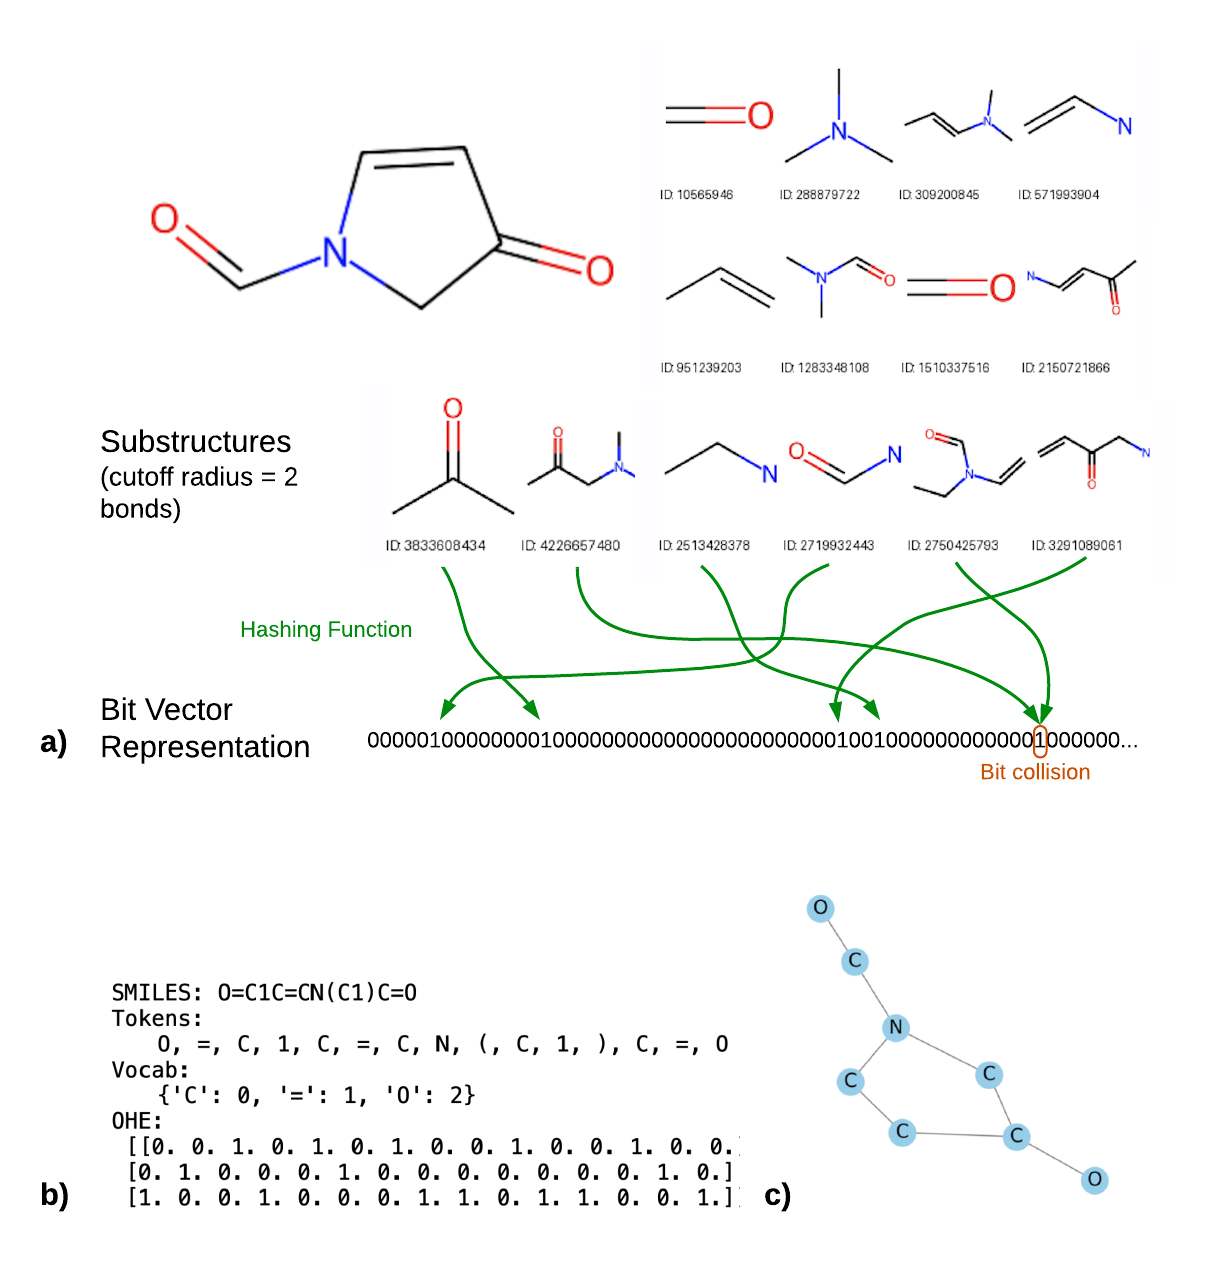
\includegraphics[width=\textwidth,height=0.72\textheight,keepaspectratio]{molecular_representations.png} % TODO: REVIEW MODIFICATION -- was 1.05\textwidth, which ran into the margin	
    \caption[Three representations of one molecule.]{\label{fig:molecular_representations}Three representations of the molecule \lstinline{O=C1C=CN(C1)C=O}. a) ECFP4, in which circular substructures up to a radius of two bonds are hashed (green arrows) to positions in a bit vector, and two substructures can share a position (bit collision, orange). b) Tokenization and one-hot encoding of the SMILES string. c) Molecular graph, with atoms as nodes and bonds as edges.}
\end{figure}

One of the most common and intuitive molecular representations is the Simplified Molecular-Input Line-Entry System (SMILES) string, which consists of a sequence of ASCII characters generated by a fixed set of rules to specify a given chemical identity \citep{Weininger1988}. A common way to use SMILES strings as inputs to QSAR models is to tokenize and one-hot-encode them rather than to use the strings themselves \citep{TeachOpenCADD2023}. The strings are tokenized into atomic branches and symbols and mapped to indices of a vocabulary, and finally converted into binary vectors using one-hot encodings \citep{TeachOpenCADD2023}. This representation, referred to as one-hot-encoded SMILES, allows models to process molecular structures as bit-vector-based fingerprints or as sequences of vectors. Sequence-based models such as recurrent neural networks and transformers have proven to be particularly successful in capturing text semantics within a sequence. When applied to raw or one-hot-encoded SMILES strings, these models can effectively capture the structure of the molecule in its textual representation \citep{TeachOpenCADD2023}. 

Another common representation is the molecular fingerprint, a vector containing information about the properties of the molecule in question. In a typical bit vector-based fingerprint, each bit accounts for the presence (1) or absence (0) of a given chemical feature or substructure \citep{Fassio2022}. One common fingerprint is the Molecular ACCess System (MACCS) key, a substructure key-based fingerprint that encodes predefined atom symbols and properties, as well as bond types \citep{Xie2020}. Another is the Extended Connectivity Fingerprint (ECFP), which encodes local neighborhoods around each atom and bond connectivity in molecules \citep{Xie2020}. ECFPs are typically constructed with a radius of 2, a length of 2048 bits, and active chirality flags. These existing molecular representations are well established and have been quite successful when coupled with QSAR models \citep{CortsCiriano2020, Sabando2021}. They are relatively simple, and as the bits can be mapped back to one or more substructures, they are human-interpretable, and furthermore easy-to-compute. However, they are subject to information loss due to bit collisions, which happens when two different substructures are encoded at the same bit position \citep{Fassio2022}. They are also based on a fixed procedure and are not trainable or adaptable to a particular dataset. Alternative representations that capture different structural, chemical, or physical features are able to overcome these limitations. 

Recent advances have led to the development of new molecular fingerprints. One such method is the Sort \& Slice (SNS) technique, an alternative to hash-based folding for pooling ECFP substructures \citep{sns}. Sort \& Slice begins by sorting all circular substructures in the training set according to their frequency of occurrence. It then ``slices'' away all but the $N$ most frequent substructures, which are subsequently used to generate an $N$-dimensional, bit-collision-free binary fingerprint. This approach solves the ambiguity problem of hashed fingerprints, where multiple substructures might be encoded at the same bit position, making it very interpretable \citep{sns}. Sort \& Slice fingerprints outperform ECFP of diameter four (ECFP4) with standard hash-based folding methods across various molecular property prediction tasks. These experiments consisted of different data splitting techniques, machine learning models, fingerprint diameters, fingerprint dimensions, and atomic invariants \citep{sns}. Furthermore, Sort \& Slice outperformed advanced substructure selection schemes such as filtered fingerprints and mutual information maximization \citep{sns}. 


Neural fingerprints are a category of learned  representations that overcome the fixed, hard-coded nature of traditional fingerprints. Unlike ECFP or MACCS keys, which rely on predefined hashing schemes or substructure catalogs, neural fingerprints train on molecular data to capture chemical information \citep{Jaeger2018, Chithrananda2020}. These representations are the result of deep learning architectures that have learned dense, continuous embeddings which can be used for downstream tasks. 

% TODO: review, needs manual review
Mol2vec, a common neural fingerprint, adapts the Word2vec algorithm from natural language processing (NLP) to molecular substructures \citep{Jaeger2018}. It treats molecules as ``sentences'' and the circular substructures from which ECFPs are built as ``words'', and it learns an embedding for each substructure through unsupervised training, such that chemically similar substructures are mapped to nearby points in the embedding space \citep{Jaeger2018}. The embeddings of all substructures present in a molecule are summed to give a 300-dimensional dense vector that represents the whole molecule \citep{Jaeger2018}. Mol2vec has performed strongly on various QSAR benchmarks, matching or exceeding ECFPs on solubility and bioactivity prediction tasks \citep{Jaeger2018}.

Transformer-based architectures have also been applied to molecular representation learning, similarly stemming from NLP ideas. MolBERT applies a bidirectional transformer to learn molecular representations from SMILES strings through self-supervised pre-training \citep{Fabian2020}. The model has domain-relevant auxiliary adaptations, such as the prediction of calculated physicochemical properties alongside the masked token prediction, to improve the chemical fidelity of the learned embeddings \citep{Fabian2020}. MolBERT demonstrated improvements over traditional fingerprints and graph-based methods on virtual screening and QSAR benchmarks \citep{Fabian2020}. ChemBERTa is another transformer-based approach which pre-trains masked language models on SMILES data from PubChem \citep{Chithrananda2020}.  ChemBERTa uses a tokenization strategy adapted for the SMILES notation, which allows the model to learn representations of atoms and functional groups through self-supervised learning \citep{Chithrananda2020}. Attention visualization reveals that ChemBERTa learns chemically meaningful patterns, with different attention heads specializing in functional groups, ring structures, or SMILES syntax \citep{Chithrananda2020}. ChemBERTa-2, an optimized variant pre-trained on 77 million compounds, achieved even stronger performance than the original ChemBERTa in MoleculeNet benchmarks \citep{Ahmad2022}.

Neural fingerprints provide several advantages over traditional fingerprints. They produce dense continuous vectors that avoid sparseness and information loss from bit collisions \citep{Jaeger2018}. They can also be pre-trained once on large unlabeled datasets and then fine-tuned for specific downstream tasks, opening the door to transfer learning \citep{Chithrananda2020, Fabian2020}. However, these methods are often computationally expensive \citep{Jaeger2018} and due to their black-box nature, they are not as interpretable \citep{Chithrananda2020}, although attention mechanisms offer some interpretability through visualization \citep{Chithrananda2020}.

Beyond fingerprints, physicochemical-descriptor vectors (PDVs) are a class of continuous-value molecular descriptors that encode structural and chemical properties of molecules \citep{Todeschini2009}. Unlike binary fingerprints or graph-based representations, PDVs aggregate atom and bond-level quantities into fixed-length feature vectors that capture a wide variety of information about a molecule and its structure \citep{Mauri2006}. PDVs typically consist of hundreds of properties including constitutional descriptors such as molecular weight, atom and bond counts, and heteroatom ratios; topological indices encoding molecular connectivity patterns; physicochemical properties such as logP (lipophilicity), molar refractivity, and topological polar surface area; and electronic descriptors derived from partial charges and polarizabilities \citep{Todeschini2009, Cherkasov2014}. The \texttt{RDKit} cheminformatics toolkit provides a comprehensive suite of more than 200 molecular descriptors that cover these categories \citep{rdkit}. PDVs are very interpretable; each descriptor has a clear physicochemical meaning \citep{Cherkasov2014}. They are also less computationally expensive than some 3D methods or neural fingerprints, with many descriptors simply requiring a 2D molecular structure without conformer generation or extensive pre-training. This efficiency makes PDVs particularly appropriate for high-throughput applications. Descriptors based on 3D structure can also be used \citep{Mauri2006}.

However, PDVs have limitations. The dimensionality of PDV feature spaces can lead to problems with multicollinearity \citep{Todeschini2009}. This can be mitigated by feature selection or dimensionality reduction techniques \citep{Cherkasov2014}. Additionally, PDVs encode molecular properties as aggregated global features, which may not capture fine-grained structural details such as specific substructure arrangements or local chemical environments, information important for particular endpoints \citep{Mauri2006}.

One of the more intuitive representations is the molecular graph. These graphs can be categorized into 2D and 3D graphs. 2D graphs rely on adjacency matrices that encode topological atom- and bond-level features but leave out geometric properties such as bond angles or torsion, meaning they may fail to capture stereochemistry. 3D graphs incorporate these spatial features, but are often limited by remaining in a single conformation \citep{Zhichun2023}. A standard molecular graph is constructed such that each molecule is represented as $G = (V,E)$ with node features $\mathbf{x}_i$ and edge features $\mathbf{e}_{ij}$. Nodes encode atom type, degree, hybridization, aromaticity, and formal charge; edges encode bond order and conjugation \citep{Zhichun2023}. 

% TODO: review, needs manual review
Another common molecular graph is the standard distance compatibility graph, in which atoms and bonds are mapped to sets of nodes and edges \citep{David2020, Hnig2022}. These graphs are typically 2D objects that encode 3D information such as atomic coordinates, bond angles and chirality \citep{David2020}. Alternative graph representations that incorporate 3D structure and physical interactions include graphs with quantum 3D embeddings, weight alignment graphs, association graphs containing pairs of molecules, and geometric interaction graph neural networks \citep{Hnig2022, yan2023, Yang2023GIGN}. \citet{Du2022} combined 2D and 3D graphs in a zipper-like arrangement, in which the 3D data guarantee precision and completeness by providing unabridged information and the 2D data provide chemical intuition for guidance. Grid-based 3D representations pose a related challenge: atoms localized at single voxels leave the grid too sparse, which leads to poor performance. \citet{Kuzminykh2018} addressed this problem by extending each atom to fill nearby voxels with a wave transformation.
      
These graph representations do not highlight specific substructures or specific arrangements of atoms and bonds within each molecule. The substructures contain functional groups that are related to a range of chemical properties and are potentially involved in downstream tasks related to the function of molecules. \citet{Bouritsas2023} developed graph substructure networks, a topologically aware message passing scheme based on substructure encoding. The method involves encoding structural roles based on the appearance of specific substructures and using them in message passing updates. Since message-passing graph neural networks (GNNs) are at most as powerful as the Weisfeiler--Lehman test, they cannot isolate sufficient features from the graph structure \citep{Bouritsas2023}. Graph substructure networks, on the other hand, capture these substructure-related features. Pretrained GNN encoders can also produce embeddings that capture structural features from unlabeled data \citep{kishimoto2023, ross2022}. 

\section{Models for Molecular Property Prediction}
% [notes moved to thesis_notes_moved.md]

There are a wide variety of model architectures that can be used for QSAR modeling. Starting off with simpler and more explainable models, we have tree-based methods. Decision trees are non-parametric supervised learning algorithms that perform recursive binary partitioning of the feature space \citep{Breiman1984}. A decision tree builds a predictive model by learning a series of if-then rules that recursively split the data based on given feature values, creating a tree  where internal nodes represent decision rules, branches represent the results of those decisions, and leaf nodes contain predicted values or class labels \citep{Breiman1984}. Each recursive split is chosen to maximize  homogeneity within the resulting partitions. For classification, Gini impurity is commonly used and for regression, mean squared error reduction \citep{Breiman1984}.

There are several properties that make decision trees a good foundation for QSAR modeling. First, they handle non-linear relationships between molecular descriptors and target properties without requiring explicit feature engineering or transformation \citep{Breiman1984}. They also do not make assumptions about the underlying distribution of the data, making them robust to violations of parametric assumptions that can limit linear regression or other classical methods \citep{Svetnik2003}. 

Decision trees handle data in a ``contributory'' rather than ``consensus'' manner. In consensus methods such as linear regression or neural networks, every data point influences the prediction at every other point in the feature space. Tree-based methods make predictions based on the subset of training samples that fall into the same leaf node as the test point \citep{Breiman1984}. This mechanism essentially quarantines outliers in their respective leaf nodes, limiting their impact on predictions for samples in other regions or chemical domains. 

% TODO: review, needs manual review
Individual decision trees tend to have high variance and often overfit, particularly at large depths \citep{Breiman1984}. Small modifications made to the training data can result in large differences in the structure of the tree, resulting in unstable predictions \citep{Breiman2001}. Ensemble methods are used to counteract this instability, aggregating predictions from many trees. Random forests (RFs) aggregate predictions from trees trained on bootstrap samples of data with random subsets of features at each split \citep{Breiman2001}. Bootstrapping ensures that each tree is trained on a slightly different subset of data, which effectively reduces the influence of any individual sample \citep{Breiman2001}. This is especially beneficial with noisy samples. The selection of random features at every node decorrelates the trees, preventing systematic biases from propagating through the ensemble \citep{Breiman2001}. The aggregation of trees further prevents overfitting to noise by smoothing out prediction errors from individual noisy labels. 

% TODO: review, needs manual review
Neural networks (NNs), a very popular family of models, can also be used for QSAR. An NN is a system of interconnected nodes which learn by passing information through its layers. There are weights and biases attached to the nodes and various other parameters which the model optimizes to minimize the difference between the predicted output and the actual target value. During training, the network parameters are updated using backpropagation, in which gradients of the loss function with respect to each weight are propagated backward through the network \citep{Rumelhart1986}. The structure of these networks and the hyperparameters used depend on the type of NN. In QSAR, one of the most commonly used architectures is the multilayer perceptron (MLP), a NN containing fully-connected layers with non-linear activation functions which transforms molecular feature vectors (i.e., fingerprints, descriptors) into a property or activity prediction \citep{Ma2015}.

For molecular property prediction, it is recommended that architectures use 2--3 hidden layers with 128--512 units each, rectified linear unit (ReLU) activations, and dropout regularization to prevent overfitting. Training is performed using backpropagation with gradient descent optimizers such as Adam, to minimize a loss function (mean squared error for regression, cross-entropy for classification) on batches of training data \citep{wu2018}. 

% TODO: review, needs manual review
However, NN performance on QSAR-related tasks has been very mixed. They are often outperformed by more traditional methods: decision trees and related ensemble models tend to perform better on smaller datasets and to overfit less \citep{Baskin2008, Koutsoukas2017}. Their complexity and use of gradients make them prone to label memorization \citep{Zhang2017}, which in the context of noise is problematic, as it means that models may memorize the noise themselves. Although models that are memorizing labels may initially appear to have strong predictive performance, they cannot generalize to out-of-distribution samples properly and often provide inaccurate uncertainty estimates. Various approaches have been proposed to improve neural network robustness to label noise, including noise-robust loss functions \citep{Song2022}, confident learning to identify mislabeled examples \citep{Northcutt2021}, and regularization techniques such as mixup \citep{Zhang2018mixup} or label smoothing \citep{Szegedy2015}. 

% TODO: review, needs manual review
All the models up to this point have assumed a vector-based input. Molecular graphs, on the other hand, require different types of predictive modeling. Two standard ML methods on molecular graphs include Graph Convolutional Networks (GCNs) and Graph Isomorphism Networks (GINs). GCNs apply the concept of convolution to graph-structured data. Instead of operating on grid-based data, such as images, GCNs aggregate information from neighbors of a node to update its representation \citep{TeachOpenCADD2023, Xu2019}. In contrast, GINs address the limitations in GCNs’ ability to differentiate between non-isomorphic graphs. Unlike GCNs, which normalize and weight the sum of neighboring node features, GINs use a simple sum followed by a trainable MLP, giving the model flexibility to learn complex transformations of node features. The GIN model’s design is informed by the Weisfeiler--Lehman test for graph isomorphism, enabling it to distinguish between molecular graphs that are structurally similar but differ in subtle ways \citep{TeachOpenCADD2023, Xu2019}. This makes GINs a candidate for modeling activity cliffs (Section~\ref{sec:mol_similarity}), where small variations in molecular structure can lead to significant changes in chemical or biological activity \citep{TeachOpenCADD2023}. 


\subsection{Tree Ensembles}
% [notes moved to thesis_notes_moved.md]


% TODO: review, needs manual review
Quantile Regression Forests (QRFs) extend RFs by holding the distribution of training labels in each leaf and computing quantiles over all trees \citep{Meinshausen2006}.

% TODO: review, needs manual review
Gradient boosting methods such as eXtreme Gradient Boosting (XGBoost) sequentially fit trees to the residuals of previous iterations, progressively reducing the prediction error \citep{Chen2016, Mustapha2016, Tian2022}. Other gradient-boosted tree ensembles include Light Gradient-Boosting Machine (LightGBM) \citep{ke2017lightgbm}, and Natural Gradient Boosting (NGBoost) \citep{Duan2020}. NGBoost extends deterministic gradient boosting by treating the parameters of a chosen parametric distribution as regression targets and learns them through boosting with a natural gradient update rule \citep{Duan2020}.


\subsection{Support Vector Machines}
% [notes moved to thesis_notes_moved.md]
% - Answer to your TODO: Chapter 3 reports how the SVM holds up under each noise condition. Point there; do not restate the numbers.

% TODO: review, needs manual review
Support vector machines (SVMs) are a well-established baseline in QSAR modeling, mapping inputs into a high-dimensional feature space in which, for classification, a maximum-margin hyperplane separates the classes \citep{Vapnik1995, Svetnik2003}.
% TODO: anything interesting to say on SVMs? Background? promising results with noise (it's actually one of the top performing in my results)
% Limitations - compute too high on large N

% CODE INPUT
% TODO: review, needs manual review
Support vector regression fits a function that is as flat as possible while keeping training errors small \citep{Vapnik1995, Smola2004}. It uses the $\epsilon$-insensitive loss, under which errors smaller than $\epsilon$ cost nothing and larger errors cost their size minus $\epsilon$. A constant $C$ trades flatness against tolerance of large errors \citep{Cortes1995}. The features enter the model only through the kernel. With the radial basis function (RBF) kernel, the kernel is a function of the Euclidean distance, so every feature enters every distance. In Chapter~\ref{chap:robustness} the continuous representations are standardized and the binary fingerprints are used as built. Three properties of the method suggest robustness to label noise. Errors inside the $\epsilon$ tube change nothing, the loss outside the tube grows linearly rather than quadratically, and the weight of each molecule is capped at $C$ \citep{Smola2004}. Under simulated experimental error, the RBF-kernel SVM degraded smoothly and linearly \citep{Cortes2015}, and Chapter~\ref{chap:robustness} reports how it holds up under each of our noise conditions. Its main limitation is computational cost, because training operates on a kernel matrix that grows with the square of the number of training molecules \citep{Chang2011}.


\subsection{Gaussian Processes}
% [notes moved to thesis_notes_moved.md]

Gaussian processes (GPs) are a non-parametric class of models that use a kernel to produce a Gaussian predictive distribution over every data point \citep{Obrezanova2007, Rasmussen2005}. One of the major limitations of using GPs in practice is computational scaling; inference has $O(N^3)$ time complexity and $O(N^2)$ memory, where $N$ is the number of training points \citep{Rasmussen2005}. This can be mitigated with sparse GP approximations, but these introduce approximation error and can be more difficult to tune \citep{quinonero2005}.


% TODO: review, needs manual review
The \texttt{Gauche} framework \citep{gauche} defines kernels for strings, fingerprints, and graphs that operate on a range of widely used molecular representations. The Tanimoto kernel \citep{Ralaivola2005, moss2020} is defined for binary vectors $\mathbf{x}, \mathbf{x}' \in \{0, 1\}^d$ for $d \geq 1$ as:

% CODE INPUT: $$...$$ changed to an equation environment with a label, so Chapter 4 can refer to it. Needs review.
\begin{equation}
k_{\text{Tanimoto}}(\mathbf{x}, \mathbf{x}') := \sigma_f^2 \cdot \frac{\langle \mathbf{x}, \mathbf{x}' \rangle}{\|\mathbf{x}\|^2 + \|\mathbf{x}'\|^2 - \langle \mathbf{x}, \mathbf{x}' \rangle},
\label{eq:tanimoto_kernel}
\end{equation}

where $\|\cdot\|$ represents the Euclidean norm \citep{gauche}. 

% TODO: review, needs manual review
The RBF kernel is defined for
$\mathbf{x}, \mathbf{x}' \in \mathbb{R}^d$ as:

\begin{equation}
k_{\text{RBF}}(\mathbf{x}, \mathbf{x}') := \sigma_f^2 \cdot \exp\left(-\frac{\|\mathbf{x} - \mathbf{x}'\|^2}{2\ell^2}\right),
\end{equation}

where $\ell$ is the lengthscale and $\sigma_f^2$ the signal variance, which scales both kernels.


\subsection{Bayesian Neural Networks}
% [notes moved to thesis_notes_moved.md]
% - Answer to your TODO: keep the paragraph. It is the only definition of the two parts in the thesis, and Chapter 3 uses both for every probabilistic model.

NNs are often deterministic; however, they can be transformed into probabilistic models (Figure~\ref{fig:bayesian_transformation}).

\begin{figure}[!htbp]
    \centering
    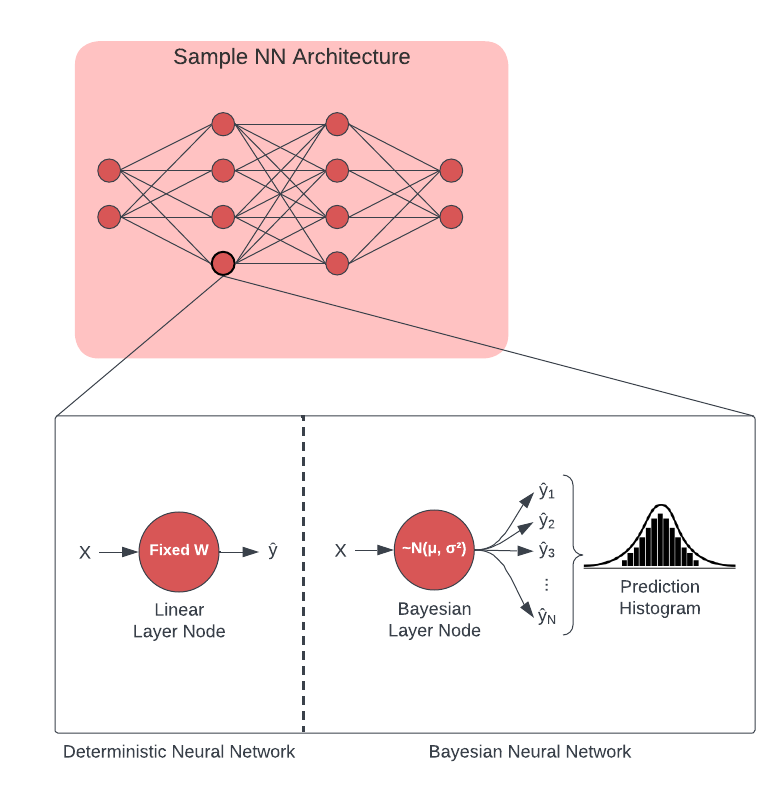
\includegraphics[width=0.85\textwidth,height=0.72\textheight,keepaspectratio]{bayesian_transformation.png}
    \caption[Nodes of a deterministic and a Bayesian neural network.]{One node of a deterministic and of a Bayesian neural network. The deterministic node (bottom left) applies a fixed weight $W$ and returns one prediction $\hat{y}$. The Bayesian node (bottom right) draws its weight from $\mathcal{N}(\mu, \sigma^2)$, so repeated predictions $\hat{y}_1, \dots, \hat{y}_N$ form a histogram.}
    \label{fig:bayesian_transformation}
\end{figure}

Unlike standard deterministic ML methods, Bayesian methods model distributions over predictions using Bayes' rule, allowing for the quantification of uncertainty within parameters and labels. Bayesian methods treat the model parameters as random variables with distributions. Uncertainty can also be estimated from other non-deterministic methods, including deep ensembles \citep{lakshminarayanan2017}, bootstrap modeling \citep{palmer2022}, and federated learning \citep{Hanser2023}.

% TODO: this paragraph may need to go
Epistemic uncertainty is model-driven and can be reduced by collecting either more or higher quality training data. Aleatoric uncertainty is data-driven and reflects the intrinsic noise in the labels.

\section{Molecular Similarity and Activity Cliffs}\label{sec:mol_similarity}
% [notes moved to thesis_notes_moved.md]
% - Answer to your TODO on the bib: the entries are in refs.bib. Still to fix: Dablander2023 lists "Michael Dablander"; it should be Markus Dablander.

% TODO: hand edit
% TODO: review, needs manual review
Much of cheminformatics rests on the similar property principle, which states that structurally similar molecules tend to have similar properties \citep{Johnson1990, vanTilborg2022}.
One of its clearest applications is nearest-neighbor prediction, which appears across cheminformatics workflows and, in this thesis, in the kernels used by GPs and at the basis of many noise identification algorithms.

% TODO: review, needs manual review
The difficulty with this principle is that similarity is defined only relative to a similarity measure, which is fixed by the choice of representation and
coefficient \citep{Maggiora2014}. There is no standard definition of similarity between molecules, especially when different molecular embeddings are handled in a computational setting. Two molecules that are near-identical under a substructure fingerprint may be far apart under a PDV, and \citet{Maggiora2014} caution that quantified similarity can be over-interpreted in this way.

% CODE INPUT: formula added so that Chapter 4's argument about distances has its starting point here
The most common measure for binary fingerprints is the Tanimoto coefficient \citep{Bajusz2015}. For two molecules with fingerprints $\mathbf{x}, \mathbf{x}' \in \{0,1\}^d$,
\begin{equation}
T(\mathbf{x}, \mathbf{x}') = \frac{\sum_{j=1}^{d} x_j x'_j}{\sum_{j=1}^{d} x_j + \sum_{j=1}^{d} x'_j - \sum_{j=1}^{d} x_j x'_j},
\label{eq:tanimoto}
\end{equation}
which is the number of bits set in both molecules divided by the number of bits set in either. Continuous representations are instead compared with a distance, most often the Euclidean distance $\sqrt{\sum_{j=1}^{d}(x_j - x'_j)^2}$. Both measures are sums over the features, and neither weighs a feature by its relation to the property. In the Tanimoto coefficient, a bit that is off in both molecules contributes nothing, whereas every bit that is set in either molecule counts. In the Euclidean distance, every feature that differs between the two molecules counts. Chapter~\ref{chap:flaws} returns to this point (Equation~\ref{eq:distance_split}).

% TODO: review, needs manual review
Distance-based reasoning relies on the assumption that the data embeddings contain quality information. When the labels are corrupted or few features relate to the property, similarity scores are dominated by features that carry no information about it, and the assumption that similar molecules have similar properties breaks down. % TODO: REVIEW MODIFICATION -- removed a doubled "et al." and a repeated citation of Bajusz2015.
\citet{Bajusz2015} found that while the Tanimoto coefficient can be effective with binary fingerprints, changing the similarity formula yields minimal improvement if the underlying representation is weak.
This problem is further complicated by activity cliffs, defined below, which potentially contain the most important information for model prediction but can be confused with noise. Another barrier to distance-based reasoning is persistent noise across labels. The task of trying to determine if a molecule's value matches that of its neighbors becomes a lot harder when all of the neighbors have some form of noise as well.

There are many downstream tasks which rely on the concept of similarity. The second half of this thesis relies on many such tasks, and as such focuses on identifying representations that agree with this principle. 


% TODO: review, needs manual review
The sharpest failure of the similar property principle is the activity cliff, a pair of structurally similar molecules with a large difference in potency that is produced by a small
chemical change \citep{Maggiora2006, Stumpfe2012}. Activity cliffs inherit the measure dependence of the principle they violate, and there is no widely accepted definition of one
\citep{vanTilborg2022}. The MoleculeACE benchmark \citep{vanTilborg2022} makes this choice explicit. A pair is considered highly similar if its similarity exceeds 90\% under at least one of
three measures, namely the Tanimoto coefficient on ECFPs, the Tanimoto coefficient on scaffold fingerprints and a scaled Levenshtein distance on SMILES strings. Such a pair forms a cliff if
the two molecules also differ tenfold or more in $K_i$ or EC$_{50}$ \citep{vanTilborg2022}. This soft consensus over three measures is used because each measure captures only part of the
underlying chemistry. Across the thirty MoleculeACE targets, cliff compounds account for between 7\% and 52\% of a dataset \citep{vanTilborg2022}.

% TODO: review, needs manual review
Dimensionality itself poses a further difficulty. \citet{Aggarwal2001} show that as the number of dimensions grows, the distances to the nearest and to the furthest
point become increasingly similar, so that pairwise distances become progressively less discriminative. Molecular representations are routinely high-dimensional and sparse, and when a
large proportion of their dimensions carry no information relevant to the property being modeled, distances computed over them are dominated by those uninformative dimensions.


% TODO: make changes to bib

\section{Noise in Molecular Data}
% [notes moved to thesis_notes_moved.md]

% TODO: review, needs manual review
Real-world cheminformatics datasets contain label noise arising from multiple sources across the drug discovery pipeline, and modeling experimental noise properly requires first understanding where it comes from.

% moved here from the start of the Models section (2026-09-30)
% TODO: review, needs manual review
One key issue with QSAR models is the standard assumption that labels represent true values. Most ML models rely on the assumption that the training data is, in fact, an accurate reflection of the population. Therefore, they treat these potentially noisy labels as exact point values rather than as draws from a distribution, which opens the door to overfitting to noise and giving unduly optimistic assessments of the models.

Studies involving noise, and specifically the quantification of noise robustness, typically approach label noise by adding independent, zero-mean, Gaussian error to the labels. However, there is evidence that noise from experimental assays takes on different forms. \citet{Kruger2012} rejected normality of bioactivity differences by Anderson-Darling test and fitted a Laplace distribution instead. \citet{Kalliokoski2013} examined the widest disagreements among 16,844 pairs of repeat pIC$_{50}$ measurements and found that in almost all cases, the wide gap between repeat values was due to annotation error rather than to an imprecise assay.

% TODO: review, needs manual review
\citet{Kolmar2021} examined the predictive limits of QSAR in the presence of noise and showed that, by learning the underlying trends rather than fitting the noise, models can make predictions that are more accurate than their own training labels. They assumed that experimental noise is Gaussian, arguing from the central limit theorem that measurements aggregated over multiple independent error sources follow a Gaussian distribution. \citet{Heid2023}, however, used mean-variance estimation and bias-variance decomposition to show that noise can be tied to specific properties of the molecules, such as their structure. For example, nitrogen-containing functional groups introduce measurement deviations, which implies the presence of systematic noise.

% TODO: review, needs manual review (last sentence adapted from paper.tex to point to Chapter 3)
% TODO: review, needs manual review
Beyond just the distribution, the assumptions of independence and zero mean may fail as well. \citet{Bentz2013} examined P-glycoprotein transport measurements across 23 laboratories and found that $62\%$ of the variance in log efflux ratio was due to differences between laboratories. When data are pooled from different sources, each source can carry a shared offset. These sources usually contain families of related compounds, breaking the independence assumption. The zero-mean assumption is not assured either, especially when true values fall above or below an assay's detection limit, called censoring. \citet{Svensson2025} count censored labels in fifteen industrial assays, of which thirteen carry censored labels and eight sit between a quarter and two thirds censored. Chapter~\ref{chap:robustness} tests noise conditions that vary the distribution, the correlation, and the bias of injected error separately, at a matched quantity of noise for every condition except censoring.

% TODO: REVIEW MODIFICATION -- the six paragraphs on noise sources are now Table tab:noise_sources. Every example and citation in the table is from those paragraphs; originals kept below.
% Assay-related variability represents a primary source of label noise in bioactivity data. High-throughput screening assays are often laden with errors from physical phenomena such as edge effects, where compounds in wells exhibit different activities at plate boundaries due to evaporation or temperature gradients \citep{Macarron2011}. Other examples include compound carryover between wells, incomplete liquid transfers, and air bubbles  \citep{Inglese2006}.  Detection reagents or unstable compounds can degrade over time, which leads to drift within a single plate run. This turns into heteroscedastic noise correlated with plate position or read time \citep{Brideau2003}.
% 
% Instrument calibration and detection limits can impact measurement accuracy. Spectrophotometric assays near detection limits exhibit higher relative error, such that signal-to-noise ratios degrade for weak binders \citep{Zhang1999}. Fluorescence quenching by test compounds introduces a systematic bia in fluorescence-based assays, resulting in false negatives for potent inhibitors that accidentally get absorbed at emission wavelengths \citep{Simeonov2008}. Radiometric assays require background subtraction and decay corrections that accumulate error, particularly for low-activity compounds where the signal barely exceeds background \citep{Zhang1999}.
% 
% Another source of noise is biological variability. Even minor variations in cell culture conditions such as seeding density, plating efficiency, growth rate, and cell cycle distribution have the potential to affect downstream tasks such as cell metabolism and drug responsiveness. Even serum properties may introduce variability \citep{Hatzis2014}. The speed of cell culture passages is even found to be a significant factor in behavior \citep{Postnikova2018}. 
% 
% Data aggregation across multiple sources compounds these individual error sources. Common databases like ChEMBL, BindingDB, and PubChem aggregate measurements from hundreds of laboratories using a diverse set of protocols, compound purities, and quality control standards \citep{Gaulton2017, Gilson2016}. The $K_i$ or IC$_{50}$ values from the same compound-target pair with between 10 and 20 reported values, often end up spanning two orders of magnitude apart, making it challenging to identify the underlying ground truth \citep{Kramer2012}. All the sources of error mentioned above regarding inconsistent experimental protocols cannot be distinguished easily from the genuine underlying value without extensive, and often unrealistic amounts of metadata \citep{Fourches2016}.
% 
% 
% Federated datasets, a method of data aggregation centered around privacy protection, presents a particularly challenging situation for noise. In pharmaceutical research and beyond, companies often want to merge collective information without exposing proprietary data to competitors. One example of such platforms is Lhasa Limited's federated learning platform Effiris. Teacher models are first trained separately on confidental data, and then used to label a shared public chemical data set. Those results are consolidated into a federated student model \citep{Bassani2023}. While this is an effective approach of protecting intellectual property, it introduces additional label noise through the prediction errors of all the teacher models. There also exists aleatoric uncertainty from the underlying experimental measurements, many of which likely come from differing protocols, resulting in compounding label noise. 
% 
% Beyond the experimental setups, annotation errors in the data itself can arise from mis-registered structures, incorrect stereochemistry assignments, and salt form ambiguity \citep{Williams2017}. Public databases are estimated to contain 1-5\% structure errors from incorrect SMILES parsing, tautomer misassignment, or manual transcription mistakes during data entry \citep{Young2008}. Ambiguous protonation states and counterions create representation-level noise where chemically distinct samples are classified as the same \citep{Bento2020}.

Label noise enters bioactivity data at every step from the assay plate to the database. Table~\ref{tab:noise_sources} lists these sources, with examples of each and the kind of error each tends to produce. The kind of error describes how the error is distributed across molecules, which is the property that the noise conditions in Section~\ref{sec:noise_injection} vary.
\begin{table}[htbp]
\centering
\small
\begin{adjustbox}{max width=\textwidth,max totalheight=0.78\textheight}
\begin{tabular}{@{}P{0.16\linewidth}P{0.46\linewidth}P{0.30\linewidth}@{}}
\toprule
\textbf{Source} & \textbf{Example} & \textbf{Kind of Error} \\
\midrule
Assay & Edge effects at plate boundaries from evaporation or temperature gradients \citep{Macarron2011}; carryover between wells, incomplete liquid transfers and air bubbles \citep{Inglese2006}; reagents or compounds degrading during a run \citep{Brideau2003} & Error that varies with plate position or read time \\
Instrument & Higher relative error near a detection limit \citep{Zhang1999}; fluorescence quenching by the test compound \citep{Simeonov2008}; background subtraction in radiometric assays \citep{Zhang1999} & Larger error for weak binders; a systematic bias; labels clipped at the limit \\
Biology & Seeding density, growth rate, cell cycle and serum properties \citep{Hatzis2014}; passage speed \citep{Postnikova2018} & Variation between repeats of the same experiment \\
Aggregation across sources & ChEMBL, BindingDB and PubChem pool hundreds of laboratories \citep{Gaulton2017, Gilson2016}; $K_i$ or IC$_{50}$ values for one compound--target pair spanning two orders of magnitude \citep{Kramer2012} & An offset shared by each laboratory or source, hard to separate from the true value without metadata \citep{Fourches2016} \\
Federated learning & Teacher models label a shared public set, and a student model learns from those labels \citep{Bassani2023} & The teachers' prediction errors on top of the measurement error \\
Annotation & Mis-registered structures, wrong stereochemistry and salt forms \citep{Williams2017}; 1--5\% structure errors in public databases \citep{Young2008}; ambiguous protonation states and counterions \citep{Bento2020} & A label attached to the wrong molecule; distinct molecules merged \\
\bottomrule
\end{tabular}
\end{adjustbox}
\caption[Sources of label noise in bioactivity data.]{Sources of label noise in bioactivity data, with reported examples and the kind of error each source produces.}
\label{tab:noise_sources}
\end{table}

% CODE INPUT: first person changed to "we"
% TODO: review, needs manual review
These sources of noise can interact with one another and produce errors that a simple Gaussian does not describe. Real-world noise, unlike the independent Gaussian noise usually injected in robustness studies, is neither independent, identically distributed, nor symmetric \citep{Heid2023}. We address this complexity by examining several ways of both modeling noise and adding it to datasets.

% TODO: review, needs manual review
Although the general assumption in much of the noise analysis and mitigation literature is that noise, specifically label noise, will have a negative effect on the model, this is not necessarily the case. There are multiple instances of using noise as a method of regularization. Although not the optimal approach to counteracting overfitting in linear regression, adding artificial noise to labels is considered a form of regularization \citep{Ullah2024}. Furthermore, adding artificial noise drawn from a Gaussian distribution to the activation layers of a neural network is considered another form of regularization \citep{Camuto2021}. Label noise may therefore act as a regularizer in some QSAR and quantitative structure--property relationship models.

\subsection{Artificial Noise Injection}\label{sec:noise_injection}
% [notes moved to thesis_notes_moved.md]
% - Answer to your TODO on the 20\%: no published estimate exists of how large a share of a dataset a difference between laboratories affects. So 20\% of molecules was chosen, not sourced. Whole scaffold families are drawn until about 20\% of the split is covered.

% TODO: review, needs manual review
To evaluate the robustness of QSAR models against label noise, we inject artificial noise into the training labels, while test labels remain free of noise. Validation labels receive noise of the same type and quantity as the training labels, drawn independently. The noise conditions are designed to mimic particular features of real experimental noise. The clean target label $y_i$ is replaced by a noisy label $\tilde{y}_i = y_i + \epsilon_i$, where $\epsilon_i$ is the artificial noise injected at the index $i$, the value of which is determined by a specified noise strategy.

% TODO: REVIEW MODIFICATION -- the paragraph listing the seven conditions is now a two-sentence lead-in; the list moved into Table tab:noise_conditions. Original kept below.
% We explored seven methodologies of adding noise, referred to as noise conditions (Figure~\ref{fig:noise_conditions}). Three vary the shape of the distribution from which the error is drawn. These shapes include Gaussian, Student-$t$ with $\nu = 5$, and Laplace distributions. Two conditions concentrate error on specific subset of molecules; outlier isolates a random tenth of them and grouped-wider concentrates on Bemis--Murcko scaffold families. Group shifted also applies noise to scaffolds, but instead gives each scaffold its own offset rather than a wider error. The seventh, censoring, sets a limit such that every label extends past that limit is reassigned to the limit itself. 
We explored seven ways of adding noise, which we refer to as noise conditions and which are illustrated in Figure~\ref{fig:noise_conditions} and summarized in Table~\ref{tab:noise_conditions}. Three conditions vary the shape of the distribution from which the error is drawn, and three concentrate the error on some molecules or share it within Bemis--Murcko scaffold families. The seventh condition, censoring, clips labels at a limit.

\begin{figure}[!htbp]
\centering
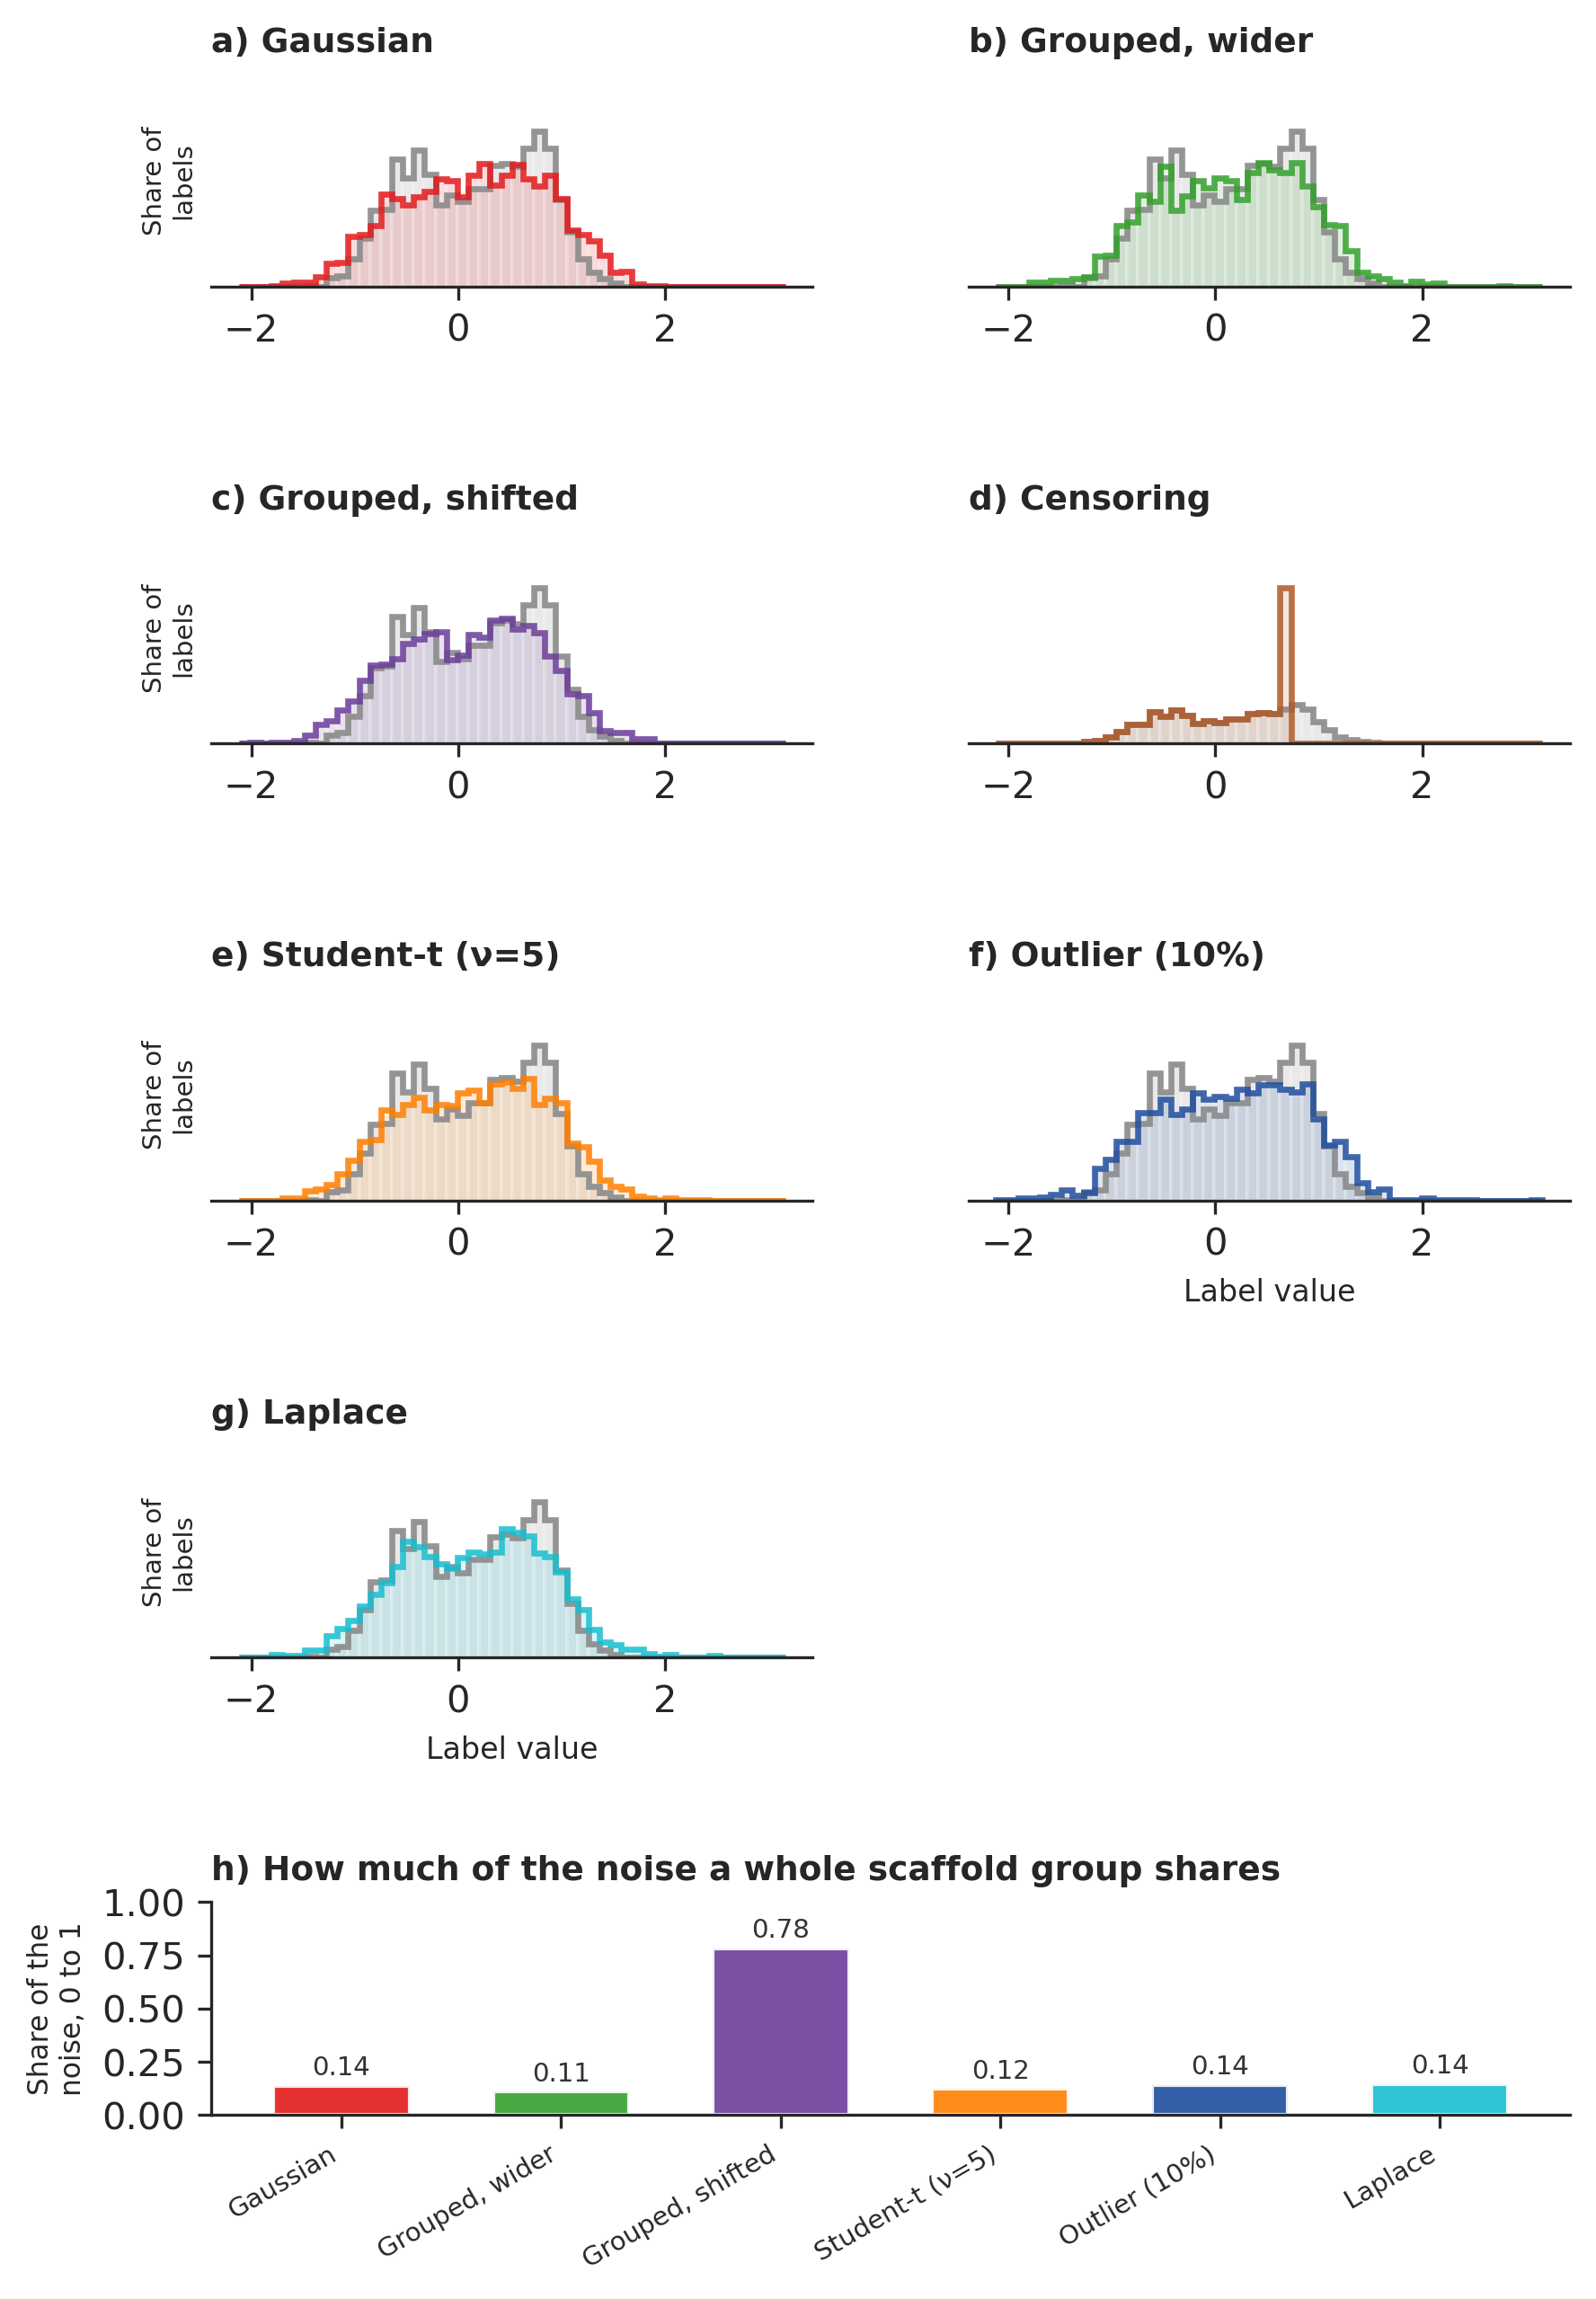
\includegraphics[width=\textwidth,height=0.72\textheight,keepaspectratio]{F1_noise_conditions.png}
\caption[Label distributions under the seven noise conditions.]{Label distributions under the seven noise conditions, for 2,000 synthetic labels in 40 random groups that stand in for scaffold families. a)--g) Clean (gray) and noised (color) labels at a noise level of 0.5 times the standard deviation of the clean labels, with 25\% of labels clipped under censoring. h) Standard deviation of the mean error within a group divided by that of all errors. A value near 1 means a group's labels move together. With about 50 labels per group, noise that ignores the groups gives about 0.14. Panel h) omits censoring.}
\label{fig:noise_conditions}
\end{figure}

% TODO: review, needs manual review
At a set noise level, every condition except censoring delivers the same expected amount of noise over the training labels. These levels are defined as a fraction of the standard deviation of the clean training labels. The noise added to the label of molecule $i$ is
\begin{equation}
\epsilon_i = \frac{\tau}{G}\,s_i z_i,
\qquad
G = \sqrt{\frac{1}{n}\sum_{j=1}^{n} s_j^{2}}\;\;\sigma_z,
\label{eq:dose_matching}
\end{equation}
% TODO: review -- paper.tex text; novelty sentence removed because it conflicts with the Heid2023 sentence in the Chapter 3 introduction.
Here $\tau$ is the target standard deviation of the noise, equal to the noise level times the standard deviation of the clean training labels, and $z_i$ is
drawn from the condition's distribution at unit scale. The multiplier $s_i$ is $1$ for most
molecules and $\lambda = 3$ for those the condition affects, which are a random $10\%$ of molecules
under outlier and whole scaffold families covering $20\%$ of the training molecules under grouped-wider. The
constant $\sigma_z$ is the standard deviation of $z$, equal to $1$ for the Gaussian,
$\sqrt{\nu/(\nu-2)}$ for the Student-$t$ and $\sqrt{2}$ for the Laplace. The factor $G$ divides both
of these out, so that $\epsilon$ has standard deviation $\tau$ in expectation whatever the
distribution and whichever molecules are affected.

Grouped-shifted widens no molecule's error, and instead gives every scaffold family $g$ an offset of
its own,
\begin{equation}
\epsilon_i = \frac{\tau}{G}\left(\sqrt{\rho}\,b_{g(i)} + \sqrt{1-\rho}\,w_i\right),
\label{eq:grouped_shifted}
\end{equation}
with one draw $b$ per family and one draw $w$ per molecule. The two variances sum to $\tau^{2}$, and
the family offset carries a share $\rho$ of that total.

% TODO: No published figure exists for the fraction of scaffold families a difference between laboratories would cover, so we chose the $20\%$ above rather than sourcing it. - need to rephrase this 
% TODO: REVIEW MODIFICATION -- the parameter paragraph is now Table tab:noise_conditions. Every value and source in the table is from this paragraph; original kept below.
% We selected parameters from published measurement errors, wherever possible. As inter-laboratory error is estimated to be approximately three times intra-laboratory error, we set $\lambda = 3$ \citep{Avdeef2019}. \citet{Hampel2001} reports that $1-10\%$ of routine scientific data contains gross errors; we selected the upper bound of $10\%$. Laboratory identity accounts for $62\%$ of the variance in Caco-2 across 23 laboratories, prompting us to set $\rho = 0.62$ \citep{Bentz2013}. We took the Student-$t$ and Laplace shapes from the distributions fitted to repeated public bioactivity measurements \citep{Kruger2012}, and contaminated a fraction of the samples with a wider error according to Huber's contamination model \citep{huber1964robust}. As we found no published estimate of how large a share of a given dataset inter-laboratory differences affect, we chose to randomly select scaffolds until $20\%$ of the molecules had been covered. 
We selected the parameter values from published measurement errors wherever possible, and Table~\ref{tab:noise_conditions} notes where no published estimate exists.
\begin{table}[htbp]
\centering
\small
\begin{adjustbox}{max width=\textwidth,max totalheight=0.78\textheight}
\begin{tabular}{@{}P{0.15\linewidth}P{0.30\linewidth}P{0.17\linewidth}P{0.30\linewidth}@{}}
\toprule
\textbf{Condition} & \textbf{What It Changes} & \textbf{Value} & \textbf{Source for the Value} \\
\midrule
Gaussian & Shape: every label's error is Gaussian & -- & The standard assumption in noise-robustness studies \\
Student-$t$ & Shape: heavier tails than Gaussian & $\nu = 5$ & Distributions fitted to repeated bioactivity measurements \citep{Kruger2012} \\
Laplace & Shape: sharper peak and heavier tails than Gaussian & -- & As for Student-$t$ \citep{Kruger2012} \\
Outlier & Error $\lambda$ times wider on a random share of molecules (Huber's contamination model \citep{huber1964robust}) & $10\%$ of molecules; $\lambda = 3$ & $1$--$10\%$ of routine data contain gross errors, upper bound taken \citep{Hampel2001}; inter-laboratory error is about three times intra-laboratory error \citep{Avdeef2019} \\
Grouped-wider & Error $\lambda$ times wider on whole scaffold families & Families covering $20\%$ of the training molecules; $\lambda = 3$ & No published estimate of the share; $\lambda$ as for outlier \citep{Avdeef2019} \\
Grouped-shifted & Every scaffold family gets its own offset; no error is widened & $\rho = 0.62$ & Laboratory identity explains $62\%$ of the variance in log efflux ratio across 23 laboratories \citep{Bentz2013} \\
Censoring & Labels past a limit are set to the limit; the level is the fraction clipped & Set by the noise level & Censored labels in industrial assays \citep{Svensson2025} \\
\bottomrule
\end{tabular}
\end{adjustbox}
\caption[The seven noise conditions and their parameters.]{The seven noise conditions and their parameter values. $\nu$ is the number of degrees of freedom of the Student-$t$ distribution, $\lambda$ the widening factor (Equation~\ref{eq:dose_matching}) and $\rho$ the share of the noise variance carried by the scaffold-family offset (Equation~\ref{eq:grouped_shifted}). For censoring, the noise level is the fraction of labels clipped.}
\label{tab:noise_conditions}
\end{table}

% TODO: review, needs manual review (caption)

% CODE INPUT: heading added so the two \ref{sec:lnl_background} in Chapters 4 and 6 resolve. Section level and title need review; no prose written.
\subsection{Learning with Noisy Labels}\label{sec:lnl_background}
% ---- NOTES: Learning with noisy labels (planned section, no heading yet) ----
% Takeaway: LNL covers every method for training a model when some labels are wrong. Noise mitigation is the subset that changes the labels before training.
% Takeaway: no single method wins, and methods that compare a molecule with its neighbors fail where similarity fails.
% Paragraph 1: what LNL is.
% - Noise mitigation changes, drops or reweights the training labels once, before a model is trained. Any model can then be fitted to the result. Examples: removal, down-weighting, smoothing, relabeling, correction.
% - Noise-robust training leaves the labels and changes how the model trains. Examples: robust losses, noise-modeling layers, regularization, and reweighting inside the training loop (co-teaching, Meta-Weight-Net).
% - A sample-selection step taken out of its training loop and used only to delete molecules before a refit counts as noise mitigation.
% - Noise detection and noise estimation find or size noisy labels. They feed noise mitigation but are not LNL methods themselves.
% - Taxonomy of 62 deep-learning methods in five groups: robust architecture, robust regularization, robust loss function, loss adjustment, sample selection \citep{Song2022}.
% Paragraph 2: why no single method wins.
% - No free lunch: averaged over all problems, no learning algorithm beats another \citep{Wolpert1996, Wolpert1997}.
% - Chemistry analog: twelve algorithms on twelve bioactivity datasets with simulated experimental errors \citep{Cortes2015}.
% - Neighbor-based cleaning goes back to editing a training set by its nearest neighbors \citep{Wilson1972}. It relies on similar molecules having similar labels, which activity cliffs break.
% - QSAR models frequently fail to predict activity cliffs \citep{Dablander2023}.
% - Chapter 6 tests this.
% ---- END NOTES ----

% CODE INPUT
LNL covers every method for training a model when some of its labels are wrong, and we divide it into two parts. Noise mitigation changes, drops or reweights the training labels once, before any model is trained, so that any model can then be fitted to the result. Its methods include removal, down-weighting, smoothing, relabeling and correction, and Figure~\ref{fig:data_cleaning} shows how such a method is evaluated. Noise-robust training instead leaves the labels unchanged and alters how the model trains, through robust losses, noise-modeling layers, regularization, or reweighting inside the training loop, as in co-teaching \citep{Han2018} and Meta-Weight-Net \citep{shu2019metaweightnet}. A sample-selection step that is taken out of its training loop and used only to delete molecules before a refit counts as noise mitigation. Noise detection and noise estimation, which find noisy labels or estimate how many there are, feed into noise mitigation but are not LNL methods themselves. \citet{Song2022} sort 62 deep-learning methods into five groups, namely robust architecture, robust regularization, robust loss function, loss adjustment and sample selection.

% CODE INPUT: figure added from ~/Downloads/Data cleaning.png. It shows the example of QM9, a Bayesian model as the
% cleaner and a random forest scored by R^2. TODO: review -- keep here as the picture of noise mitigation, or move it.
\begin{figure}[!htbp]
    \centering
    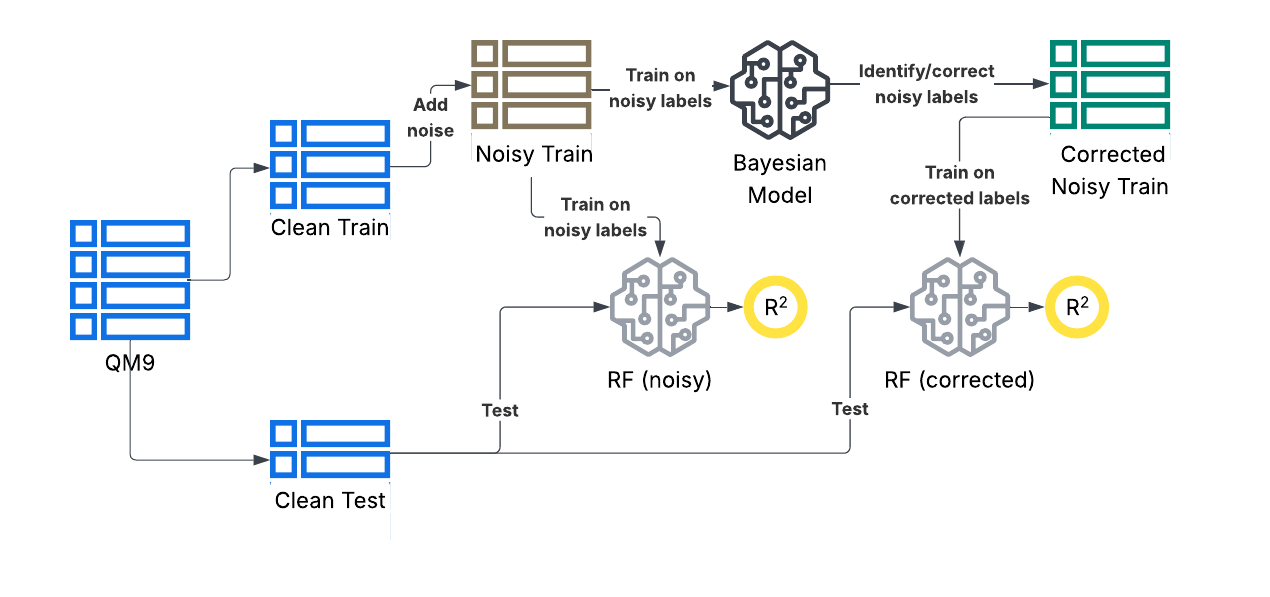
\includegraphics[width=0.95\textwidth,height=0.72\textheight,keepaspectratio]{figures_code_input/data_cleaning.png}
    \caption[Evaluation of a noise mitigation method.]{Evaluation of a noise mitigation method, with QM9 as the example. Noise is added to the training labels only. A random forest trained on the noisy labels is compared with one trained on labels corrected by a Bayesian model, and both are scored by $R^2$ on the clean test set.}
    \label{fig:data_cleaning}
\end{figure}
% CODE INPUT
% TODO: review, needs manual review (Cortes2015 details and the no-universal-solution sentence added from paper.tex)
No single method is expected to win, since averaged over all problems no learning algorithm outperforms another \citep{Wolpert1996, Wolpert1997}. The analog in chemistry is a study of twelve algorithms on twelve bioactivity datasets with simulated experimental errors at ten noise levels, which found that no single algorithm was best overall at maintaining predictive performance, and that some algorithms do better or worse at different levels of noise \citep{Cortes2015}. No single method can therefore be assumed to suit every dataset. Neighbor-based cleaning dates back to editing a training set by its nearest neighbors \citep{Wilson1972}, and it relies on similar molecules having similar labels, an assumption that activity cliffs break. QSAR models also frequently fail to predict activity cliffs \citep{Dablander2023}. Chapter~\ref{chap:flaws} tests the assumption that similar molecules have similar labels, and Chapter~\ref{chap:similarity} tests neighbor-based noise mitigation with the hybrid as the feature space.


\section{NoiseInject: A Benchmarking Framework}
% [notes moved to thesis_notes_moved.md]

% TODO: review, needs manual review
The noise conditions described above are implemented twice. NoiseInject, an open-source Python package, injects the noise on the three assay datasets and computes the robustness and uncertainty metrics, whereas QM9 uses a separate
pipeline, written in Python and Rust, that carries its own Rust implementation of the same conditions.
An automated check compares the two implementations before any experiment is run on the computing cluster. Because the random number generators of Rust and
NumPy produce different streams, the check compares statistics rather
than individual draws. On the same labels, groups and seeds, it compares the delivered noise, the
factor $G$, the median error, the number of badly corrupted labels and the number of molecules
affected.

\subsection{Package Description}\label{sec:noiseinject_pkg} % CODE INPUT: label added
% [notes moved to thesis_notes_moved.md]

% TODO: review, needs manual review
NoiseInject (version 1.0.0) evaluates model robustness and uncertainty calibration under artificial
label noise, for both regression and classification. It operates on arrays of labels and on the
predictions of any externally trained model, which makes it model-agnostic, and its core depends only
on NumPy, pandas, SciPy and scikit-learn. Results are returned as \texttt{pandas} data frames with one
row per noise level and one aggregate summary row. The software is available under an MIT license
and archived on Zenodo \citep{noiseinject}.

% TODO: review, needs manual review
\paragraph{Regression noise.} The regression injector specifies a noise shape (Gaussian, Student-$t$ or
Laplace) and a targeting rule (uniform, grouped-wider, grouped-shifted, outlier or censoring)
separately. Each named condition in the package is one combination of the two, together with its
parameters, and this name is recorded with every result. The package defines more settings
than Chapter~\ref{chap:robustness} uses, namely Student-$t$ distributions with $\nu \in \{3, 5, 10\}$ and outlier contamination of $1\%$,
$5\%$ and $10\%$ of molecules. It also defines an outlier variant in which the unselected molecules receive no
noise at all, rather than the base-scale noise of Equation~\ref{eq:dose_matching}.

% TODO: review, needs manual review
The requested noise is the root-mean-square noise $\tau$ in the units of the label, that is, the noise level times the standard deviation of the clean training labels. The
injector computes the per-molecule multipliers $s_i$ and solves for the scale $\tau / G$ in closed
form (Equation~\ref{eq:dose_matching}), so no calibration search is needed. A level of zero returns the
labels exactly unchanged. The affected molecules are selected with a second random number generator,
which is seeded separately from the noise draws and re-seeded on every call. As a result, the affected molecules are
the same at every noise level, including zero, while the noise draws themselves change. Under the
grouped-wider condition, whole scaffold families are added in random order until they cover as close as possible
to $20\%$ of the training molecules, because a fixed fraction of families
gives a very different fraction of molecules when family sizes are uneven.

% TODO: review, needs manual review
The censoring condition is parameterized by the fraction $f$ of labels clipped, and its limit is the $(1-f)$ quantile
of the clean training labels. On the training split, the censored
set is therefore exactly the $k = \mathrm{round}(fn)$ largest labels, whereas on any other split it consists of whichever
molecules lie past the training limit.

% TODO: review, needs manual review
Alongside the noisy labels, each injection returns a record of how they were produced. This record contains the target amount of noise, the factor
$G$, the solved scale, the delivered root-mean-square noise (in label units and as a fraction of the
clean label standard deviation), the mean of $\epsilon$, the fraction of molecules affected, the
number of groups and the largest share held by one group, and the random seeds. The injector also checks the delivered amount of noise.
Because the delivered amount is an estimate from a finite sample, it is compared against a band of three
standard errors,
\begin{equation}
\left|\frac{\hat{\tau}}{\tau} - 1\right| \le \max\!\left(3\sqrt{\frac{\kappa - 1}{4\,n_{\mathrm{eff}}}},\; 0.005\right),
\qquad
n_{\mathrm{eff}} = \frac{\left(\sum_i s_i^2\right)^2}{\sum_i s_i^4},
\label{eq:dose_tolerance}
\end{equation}
where $\hat{\tau}$ is the delivered root-mean-square noise and $\kappa$ is the sample kurtosis of the
unscaled draws $z$, bounded between 3 and 60. The effective count $n_{\mathrm{eff}}$ is the number of
independent contributions over which the delivered amount of noise averages, and it falls below $n$ when the noise is
concentrated on a few molecules. Under the grouped-shifted condition it is
$n_{\mathrm{eff}} = \left(\rho^2/g_{\mathrm{eff}} + (1-\rho)^2/n\right)^{-1}$, with
$g_{\mathrm{eff}} = \left(\sum_g n_g\right)^2 / \sum_g n_g^2$ for family sizes $n_g$. At
$\nu \le 4$ the Student-$t$ distribution has no fourth moment, so the standard error is instead
$1.3\,n_{\mathrm{eff}}^{\,2/\nu - 1}$, with the constant calibrated on the measured spread. A draw
outside the band raises a warning rather than an error. At three standard errors, a correct injector
falls outside the band on about $1\%$ of draws, and the delivered amount is recorded with the result
in either case.

% TODO: review, needs manual review
A second function of the package returns the noise scale that each molecule's region would receive, without drawing any noise.
We use it to score held-out molecules against the pattern of noise to which the training labels were exposed. Under the
uniform and grouped-shifted targeting rules this scale is the same for every molecule, so the package flags the result
as degenerate, because a rank correlation against a constant is undefined and must not be reported as zero.

% TODO: review, needs manual review
A separate injector sizes the noise against a unit supplied by the user rather than against the label standard
deviation. In the experiments implemented in the KIRBy repository, this unit is the standard deviation of a model's out-of-fold residuals on
the clean training labels, so that the noise is sized against the error the model already makes. Its
conditions either add Gaussian noise with variance equal to the level times the square of the unit, or move $2\%$,
$5\%$ or $10\%$ of labels by the level times the unit, with a random sign or always upward. They can also add
Gaussian noise whose standard deviation follows either a per-molecule covariate or a hidden
log-normal draw, and both of these are scaled to the same mean variance as the first condition.

% TODO: review, needs manual review
\paragraph{Classification noise.} The package provides six label-flipping strategies, namely uniform flips,
flip rates set by class frequency, asymmetric flip rates for binary tasks, a random flip rate for each sample,
a separate flip rate for each class, and flips directed by a confusion matrix. Because the realized
flip rate differs from the nominal flip probability under most of these strategies, a binary search
finds the flip probability that produces a target fraction of changed labels.

% TODO: review, needs manual review
\paragraph{Robustness metrics.} For regression, the package computes $R^2$, the root mean squared error (RMSE) and the mean absolute
error at every noise level. For classification, it computes accuracy, together with macro- and weighted-averaged precision, recall and F1
score and a per-class breakdown. Robustness is read from the
retention curve $\mathrm{ret}(x) = m(x)/m(0)$, where $m$ is a bounded metric for which higher values are better
($R^2$ for regression; accuracy, F1, precision or recall for classification) and $x$ is the noise
level. The primary summary is the normalized area under this curve,
\begin{equation}
\mathrm{AUC}_{\mathrm{norm}} = \frac{1}{x_{\max} - x_{\min}} \int_{x_{\min}}^{x_{\max}} \mathrm{ret}(x)\,\mathrm{d}x,
\label{eq:auc_norm}
\end{equation}
evaluated by the trapezoid rule. It is the mean fraction of clean performance retained across the
noise levels, lies approximately within $[0, 1]$, and is less directly correlated with clean-label $R^2$ than other robustness metrics we tested. A
secondary summary fits $\mathrm{ret}(x) \approx \exp\!\left(-(x/\tau_W)^{\beta}\right)$ to the curve. The shape parameter
$\beta$ separates curves that hold and then collapse ($\beta > 1$) from curves that fall early and
then plateau ($\beta < 1$), while $\tau_W$ sets the scale of the decay, and the fit requires at least four
noise levels. These two summaries replace the linear slope of performance against noise used in
earlier versions of NoiseInject, which misdescribed a nonlinear curve and was coupled to clean performance. The
package also reports the clean baseline and the retention at the highest noise level. A flag marks any
curve that falls below zero retention, and an optional threshold withholds the curve summaries for
models whose clean baseline is too low for a meaningful degradation.

% TODO: review, needs manual review
\paragraph{Uncertainty metrics.} For a model that returns a predicted standard deviation
$u_i$ for each sample, the package computes several metrics at each noise level. These are the Spearman correlation between $u_i$ and the
absolute error $|y_i - \hat{y}_i|$, the empirical coverage $\frac{1}{n}\sum_i \mathbb{1}\left[|y_i -
\hat{y}_i| \le k u_i\right]$ at $k = 1$ and $k = 2$ against Gaussian targets of $68.3\%$ and
$95.4\%$, the mean interval width $\frac{1}{n}\sum_i 2u_i$, and the expected calibration error (ECE),
\begin{equation}
\mathrm{ECE} = \sum_{b=1}^{10} \frac{|B_b|}{n}\,\left|\bar{u}_b - \overline{|y - \hat{y}|}_b\right|,
\label{eq:ece}
\end{equation}
computed over ten equal-count bins $B_b$ of $u$. All of these metrics are computed on the clean test labels. The Spearman
correlation between $u_i$ and the injected noise $|\epsilon_i|$ can only be computed where the noise
is known, which is on the corrupted molecules, so it requires a separate pair of inputs. It is reported
within each noise level, and a correlation pooled across all levels is returned separately. The pooled value
mostly reflects the fact that uncertainty and noise both rise with the level, so it
does not measure whether a model can identify which molecules are corrupted.

% TODO: review, needs manual review
Three optional wrappers produce $u_i$ from a point predictor. The first applies split-conformal prediction to any
scikit-learn-compatible model, optionally scaled by the label spread of each molecule's nearest
training neighbors. The second fits an exact Gaussian process with a Tanimoto or RBF kernel through \texttt{Gauche}
\citep{gauche}, and the third applies Monte Carlo dropout to any \texttt{PyTorch} network \citep{gal2016}. Example
notebooks and scripts cover regression and classification from start to finish.


\section{Evaluation Methodology}
% [notes moved to thesis_notes_moved.md]

% TODO: review, needs manual review
Chapter~\ref{chap:robustness} reports predictive performance as $R^2$ on held-out molecules and robustness as \aucnorm{} (Equation~\ref{eq:auc_norm}). Chapters~\ref{chap:flaws} to~\ref{chap:similarity} state the metric used for each dataset where it is introduced.

\section{Conclusions}

% ---- NOTES: Conclusions ----
% Takeaway: a predictor is a representation paired with a model; Chapter 3 asks which of the two governs how badly a predictor degrades under label noise.
% Paragraph 1: 3-4 sentences.
% - Sentence 1: both halves of a predictor, the representation and the model, have now been introduced.
% - Sentence 2: real assay noise is not independent, identically distributed or symmetric. The artificial noise model has seven conditions. LNL methods have been set out, with noise mitigation as the subset that acts on the labels.
% - No single LNL method wins on every dataset.
% - Sentence 3: NoiseInject injects the conditions and reports robustness and uncertainty metrics. The evaluation section fixes the splits and metrics.
% - Sentence 4: Chapter 3 asks whether the representation or the model architecture governs how badly a predictor degrades under label noise. Point to Chapter 1 for its four questions.
% - Optional: the representations, similarity definitions and noise conditions are reused in Chapters 4 to 6.
% ---- END NOTES ----

% CODE INPUT
% TODO: review, needs manual review -- splits text not yet written; notes in thesis_notes_moved.md
This chapter has introduced both halves of a predictor, namely the representation and the model. Because real assay noise is not independent, identically distributed or symmetric, our artificial noise model comprises seven conditions. We have also set out the methods for LNL, of which noise mitigation is the subset that acts on the labels, and noted that no single method wins on every dataset. NoiseInject injects these noise conditions and reports the robustness and uncertainty metrics, and the section on evaluation methodology fixes the metrics. Chapter~\ref{chap:robustness} asks whether the representation or the model architecture governs how strongly a predictor degrades under label noise, through the four questions set out in Chapter~\ref{chap:intro}. The representations, similarity definitions and noise conditions introduced here are reused in Chapters~\ref{chap:flaws} to~\ref{chap:similarity}.

\chapter{Noise Robustness Across Molecular Representations and Model Architectures}\label{chap:robustness}
% TODO: Chapter 3 update pending. When it lands, search for `TODO: Ch3 update' in Chapters 1, 4 and 7 and re-check each quoted result. Also re-check the Chapter 3 Additional files and the abstract.
% [notes moved to thesis_notes_moved.md]

% TODO: review, needs manual review
% [CODE INPUT: commented out -- the Chapter 3 paper was not submitted, so it is not referenced]
% \textit{Preamble.} The work in this chapter is adapted from Punt, A., Hanser, T., Werner, S., and Morris, G.M., in preparation for the \textit{Journal of Cheminformatics}. Most of the figures, tables, and text in this chapter are therefore either identical or similar to the content of that manuscript. A signed Statement of Authorship for this jointly authored work is included in the front matter.

\section{Introduction}
% [notes moved to thesis_notes_moved.md]


% TODO: review, needs manual review
While there have been many investigations into the effect of noise on molecular property prediction, direct comparisons of how different molecular representations respond to label noise remain limited. The choice of molecular representation affects predictive performance. \citet{Deng2023} evaluated 62,820 models and found that ECFPs frequently outperform learned graph embeddings across models. This chapter asks whether these conclusions carry over to noise robustness. Between different types of label noise, \citet{Heid2023} found no difference in model performance between error distributions with the same mean and standard deviation. We expand on this by considering alternative patterns of noise, namely noise concentrated on a sparse subset of molecules or within scaffold families, an offset shared within each scaffold family, and labels clipped at an assay limit.

% TODO: review, needs manual review
This chapter addresses the four questions set out in Chapter~\ref{chap:intro}, namely how representation and model architecture divide the variance in predictive performance and in noise robustness, what probabilistic models add, whether the type of label noise matters, and whether uncertainty estimates track label noise.

\section{Methods}\label{sec:robustness:methods}
% ---- NOTES: Methods ----
% Takeaway: the study crosses four datasets, six representations, 20 model configurations, seven noise conditions and seven noise levels.
% Paragraph 1 (only if the section gets a lead-in paragraph):
% - Four datasets: QM9 (HOMO--LUMO gap) and three assay datasets (logD, Caco-2, hERG K$_i$).
% - Six representations, 20 model configurations, seven noise conditions, seven noise levels.
% - The 20 configurations are thirteen base models and seven variant models. Name both terms here; the Models subsection defines them.
% - The noise conditions are defined in Section~\ref{sec:noise_injection}. Hyperparameters are in Additional file~\ref{app:noise:sec:hyperparameters_default}.
% ---- END NOTES ----

% CODE INPUT
% TODO: check the count of variant models. The Chapter 3 results and Additional files name six variant models on the three assay datasets (19 models ranked there), while an earlier version of this paragraph said seven (20 configurations); the paragraph now says six, following paper.tex, whose six are RF (300 trees), GP (het.), the two BNNs with a variance head and the two heteroscedastic VBLL networks. The seventh is probably the Tanimoto-kernel GP, run on ECFP4 only; not verified which count holds on QM9.
% Checked 2026-09-30: the seventh is the Tanimoto-kernel GP (`gauche`). qsar_qm_models/scripts/figlib_config.py:580-594 puts it in VARIANT_MODELS and drops it from every cross-model figure and table (RERUN_PLAN.md 14.11v); results/decisions_arc_20260916/auc_norm_assay.csv and results/decisions_arc/auc_norm_qm9.csv hold it on ECFP4 only, on all four datasets, under three noise conditions. Six is the count of variant models that are reported.
% TODO: review, needs manual review
We used four datasets, namely QM9 with the HOMO--LUMO gap as the prediction target and three assay datasets for LogD, Caco-2 and hERG $K_i$. On each dataset we paired six representations with thirteen base models and six variant models, which the Models subsection describes. Every pairing was run under Gaussian, grouped-wider and grouped-shifted noise at seven noise levels, and the other four noise conditions (Section~\ref{sec:noise_injection}) were run on selected pairings. The hyperparameters of every model are given in Additional file~\ref{app:noise:sec:hyperparameters_default}.



\subsection{Datasets}

Although we are investigating the effects of label noise stemming from experimental settings, for the purposes of testing we inject controlled amounts of artificial noise into clean labels. Data were extracted from the QM9 molecular property dataset distributed by PyTorch Geometric \citep{Ramakrishnan2014}, which contains 130,831 small organic molecules with pre-computed quantum-mechanical properties obtained from density functional theory calculations at the B3LYP/6-31G(2df,p) level of theory. We selected the HOMO--LUMO gap as the prediction target in QM9, as it captures a molecule's electronic excitability, charge transfer capability, and chemical stability \citep{Fediai2023}. We assumed that QM9 labels were free of noise, notwithstanding approximations in the level of theory. Each experiment was replicated 10 times with a distinct random seed and a randomly selected subset of $N = 10{,}000$ molecules, split 80/10/10 into 8,000 training, 1,000 validation and 1,000 test molecules. All models were fitted on those 8,000 training molecules, except the Gaussian processes, which were fitted on a random subset of 5,000 of them; the validation and test molecules were unchanged.

We repeated these experiments on three molecular property datasets with experimentally determined endpoints. From the OpenADMET initiative \citep{openadmet}, we used LogD and Caco-2 efflux permeability, with $N = 5{,}039$ and $N = 2{,}161$ respectively. We also selected hERG $K_i$ data from ChEMBL \citep{Zdrazil2023}, following a protocol inspired by \citet{landrum2024}: filter for binding assays, deduplicate by median pChEMBL value, and remove compounds with an inter-assay standard deviation greater than 1.0 log unit, resulting in $N = 1{,}415$ compounds. Each of the three was partitioned into five folds by grouped $k$-fold cross-validation, and each fold's training block gave up a further grouped fifth as a validation set for early stopping. A model therefore fits between 3,194 and 3,364 of the 5,039 LogD molecules, depending on the fold, so the Gaussian-process subsample never applies to these datasets. Unlike QM9's 10 replicates, which are 10 independent draws from one pool, each assay dataset is a single fixed set in which every molecule is tested exactly once and nothing is redrawn.

All splits and cross-validation folds were grouped by the chirality-blind Bemis--Murcko scaffold, implemented such that each distinct acyclic molecule forms its own group, and groups are filled in random order. Prior to modeling, all molecular structures were sanitized and canonicalized using \texttt{RDKit} to remove invalid valence states and standardize atom and bond typing \citep{rdkit}. Prediction targets were standardized to zero mean and unit variance. Experiments that track uncertainty were run once rather than in replicates.

\subsection{Representations}

In this chapter, we evaluated six molecular representations: ECFP4, Avalon, Sort \& Slice, PDV, ChemBERTa and Molecular Hypergraph Grammar GNNs (MHG-GNNs). The same six were used on QM9 and on the three assay datasets. ECFP4 is a Morgan fingerprint with radius $r = 2$ with $d = 2048$ bits \citep{rogers2010, rdkit}. Sort \& Slice takes the same substructures as ECFP4, but it ranks them by prevalence and selects the top $L$ ($L=1024$) \citep{sns}. We fitted the Sort \& Slice vocabulary on the training molecules alone, refitting it for each QM9 replicate and for each cross-validation fold.  Avalon is a 2,048-bit fingerprint, generated with the Avalon toolkit through RDKit \citep{avalon, rdkit}. The PDV representation is a vector of 200 physicochemical descriptors computed with RDKit's \texttt{MolecularDescriptorCalculator} \citep{rdkit, Cherkasov2014}; the 200 are listed in Additional file~\ref{app:noise:sec:pdv_descriptors}, and the list is fixed in our code rather than taken from RDKit's default descriptor set, which grows between releases. ChemBERTa embeddings are the mean over the non-padding token embeddings of the \texttt{DeepChem/ChemBERTa-77M-MTR} checkpoint, producing 384 features \citep{Ahmad2022}. MHG-GNNs are a GIN-based autoencoder pre-trained on 1.34 million PubChem molecules using a $\beta$-variational autoencoder loss, producing 1,024-dimensional embeddings through iterative message passing and found in the published \texttt{mhggnn\_pretrained\_model\_0724\_2023} checkpoint \citep{kishimoto2023}. We z-score normalized PDV, ChemBERTa and MHG-GNN per feature, using the training molecules' mean and standard deviation; ECFP4, Avalon and Sort \& Slice reach the model as built.

\subsection{Models}
% [notes moved to thesis_notes_moved.md]

To understand model behavior in the presence of label noise, we explored a range of model types (Chapter~\ref{chap:background}). We fitted tree ensembles, a support vector machine, Gaussian processes and neural networks. Several are variants of one another, differing in the probabilistic machinery they add, and Additional file~\ref{app:noise:sec:hyperparameters_default} gives every configuration with its settings.

% TODO: review, needs manual review
Among the tree ensembles, we used RFs and QRFs. While we used 100 trees for RF, we observed a noisy quantile estimate with 100 trees for QRF, prompting us to use 300 instead. To observe the effect of the quantile mechanism, we then fit a second RF at 300 trees so the two models were identical in all other settings.

% TODO: review, needs manual review
We also used XGBoost, LightGBM and NGBoost. NGBoost uses validation data for early stopping. On QM9 this is the validation split. On the three assay datasets NGBoost receives the training molecules without the validation set, and holds out a scaffold-grouped fifth of them for early stopping.

% TODO: review, needs manual review
For the SVM, we used a radial basis function (RBF) kernel with $\gamma = \texttt{scale}$ and $C = 1.0$.

% TODO: review, needs manual review
We fitted three variants of GPs, each with a constant mean and a scaled kernel. The first uses an RBF kernel and runs on all six representations. The second uses the Tanimoto kernel \citep{Ralaivola2005, moss2020}, which is defined only on binary vectors, so it was run on ECFP4 alone, on all four datasets under Gaussian, grouped-wider and grouped-shifted noise. Because it covers only one of the six representations, it is not counted among the base or variant models, and its results are not reported in this chapter. The third is a heteroscedastic variant in which the RBF process is given a second network that predicts the observation noise of each molecule. Because the cost of an exact GP grows with the cube of the number of training molecules (Chapter~\ref{chap:background}), and sparse approximations introduce approximation error and can be harder to tune \citep{quinonero2005}, we used an exact GP and fit it on at most $5{,}000$ training molecules, drawn by a seeded sample. We implemented these GP models in \texttt{GPyTorch} \citep{gpytorch}, with the Tanimoto kernel taken from the \texttt{Gauche} framework \citep{gauche}.

We tested two deterministic feed-forward architectures, both fully connected and both implemented in PyTorch \citep{Paszke2019}: (i) NN-$\alpha$ with two hidden layers of sizes 128 and 64, and dropout after each hidden layer and (ii) NN-$\beta$ with two hidden layers, each of size 128, with dropout applied before the output layer, both with ReLU activations and dropout ($p = 0.2$). Each model was trained using the Adam optimizer with early stopping on validation loss. Additional file~\ref{app:noise:sec:hyperparameters_default} gives their full widths, dropout fractions, learning rates and batch size.

% TODO: review, needs manual review
To get these networks producing uncertainty estimates, we applied four probabilistic transformations to each architecture, producing eight probabilistic networks. The first replaces every linear layer with a Bayesian layer carrying a Gaussian prior $\mathcal{N}(0, 0.1^2)$ on its weights, producing BNN-$\alpha$ and BNN-$\beta$. They are trained on an evidence lower bound whose  Kullback–Leibler (KL) divergence term is divided by the number of training molecules. The second variant adds to the Bayesian network an output head that predicts a variance and fits the negative log likelihood of a Gaussian with that variance \citep{kendall2017}. The third, Variational Bayesian Last Layer (VBLL), replaces the output layer with a layer that produces mean-field variational posteriors $q(\mathbf{W}) = \mathcal{N}(\boldsymbol{\mu}_W, \text{diag}(\boldsymbol{\sigma}_W^2))$ over the last-layer weights and trains by maximizing the evidence lower bound. This can be thought of as minimizing the reconstruction loss plus KL divergence $D_{\text{KL}}(q(\mathbf{W}) \| p(\mathbf{W}))$ from a standard normal prior, scaled by $1/N$ \citep{Harrison2024}. VBLL networks learn one observation-noise variance for the whole fit, so their aleatoric component does not vary between molecules. The fourth is a heteroscedastic VBLL network, in which the observation noise is predicted for each molecule rather than learned once for the whole fit. All eight probabilistic networks estimate their predictive distributions from 100 stochastic forward passes. Each network and its Bayesian counterpart were tuned to the same set of parameters so that NN-$\alpha$ against BNN-$\alpha$ and NN-$\beta$ against BNN-$\beta$ differ by the Bayesian layers alone.

% TODO: review, needs manual review
The thirteen base models are RF, QRF, XGBoost, LightGBM, NGBoost, SVM, the RBF-kernel GP, and NN, BNN and VBLL in each of the two architectures. The six variant models are the random forest with 300 trees, RF (300 trees); the heteroscedastic GP, GP (het.); the Bayesian networks with a variance head, BNN-$\alpha$ (var.\ head) and BNN-$\beta$ (var.\ head); and the heteroscedastic VBLL networks, VBLL-$\alpha$ (het.) and VBLL-$\beta$ (het.).

\subsection{Noise Conditions and Levels}
% [notes moved to thesis_notes_moved.md]
% TODO: review, needs manual review
The seven noise conditions used in this chapter are defined in Section~\ref{sec:noise_injection}.

% TODO: review, needs manual review
We ran experiments across seven noise levels (Section~\ref{sec:noise_injection}), $0$, $0.2$, $0.3$, $0.5$, $0.75$, $1.0$ and $1.5$. We added the noise to the raw label and standardized the target afterward, using the clean training mean and spread. For censoring, every label above the $k$th largest clean training label was set to that value, and the noise level is the fraction of training labels clipped, at $0$, $0.1$, $0.2$, $0.25$, $0.3$, $0.4$ and $0.5$ \citep{Svensson2025}.


\subsection{QM9 Data Pipeline}
% [notes moved to thesis_notes_moved.md]

% TODO: review, needs manual review
QM9 \citep{Ramakrishnan2014}, loaded through PyTorch Geometric, was processed by a separate pipeline
in which Python code loads and splits the data, computes every representation, and trains and scores
the models. Between featurization and training, a program written in Rust injects the noise,
standardizes the labels and writes the files from which the models are trained.

% TODO: review, needs manual review
Each replicate used a new scaffold split (Datasets subsection), and the same grouping defines the scaffold families targeted by the grouped noise conditions.

% TODO: review, needs manual review
The six representations described above are computed in Python. The run halts if any molecule has an ECFP4 or Avalon fingerprint
that is entirely zero, so that a molecule that failed featurization cannot enter training.

% TODO: review, needs manual review
Conventional approaches load entire datasets into memory from comma-separated values (CSV) or Parquet files, which creates memory bottlenecks at scale and repeats the cost of deserialization in every experimental replicate. Our pipeline instead serializes the preprocessed data into custom memory-mapped binary files that are read on demand, so that memory use stays low and constant regardless of dataset size (Figure~\ref{fig:fig_mmap}). Python writes one file per split, the Rust program reads each file and writes a new one in which the processed labels replace the raw ones, and Python then reads the new files back for training.

% TODO: review, needs manual review
Each memory-mapped file stores a sequence of fixed-format records. A record holds the isomeric and canonical SMILES strings in UTF-8 with a length prefix, the raw target value as a 4-byte float, the requested representations as fixed-width blocks, and the processed target value, which includes the noise and normalization, as a 4-byte float. The blocks occupy 2,048 bytes for Sort \& Slice (1,024 16-bit integers), 800 bytes for PDV (200 32-bit floats), 1,536 bytes for ChemBERTa (384 32-bit floats), 4,096 bytes for MHG-GNN (1,024 32-bit floats), and 256 bytes each for Avalon and ECFP4. Only the requested representations are written, so the byte offset of every field depends on the list of representations. This format permits zero-copy memory mapping, in which Python and Rust access the same disk-backed memory pages without deserialization.

% TODO: review, needs manual review
The Rust program draws the noise for each split separately, following the order in which that
split's records are stored. The noise parameters are set on the training split, since the amount of
noise, the censoring limit and the affected scaffold families are all computed from the clean
training labels. Validation labels receive an independent draw, from a seed derived from the
training seed, with the same amount of noise in label units, the same limit and the same affected
families, and the program verifies that validation received as much noise as training. Test labels
are never corrupted, although every split records the per-molecule noise scale its region would
have received, so that held-out molecules can be scored against the pattern applied in training.

% TODO: review, needs manual review
For every molecule in every split, the Rust program records its canonical SMILES, clean label,
injected noise, noise scale, the noise pattern applied to its region, noisy label and the
standardized value written to file. It also writes a summary of each run that lists the parameters
of the noise condition and the amount of noise delivered. The run halts if the record at any
position holds a different molecule when it is written than when its noise was drawn. A separate
self-test mode applies the same checks on the amount and targeting of noise to a label file,
without running the rest of the pipeline.

% TODO: review, needs manual review
The pipeline then trains the models described in the Models subsection, with the default and tuned hyperparameters given in Additional file~\ref{app:noise:sec:hyperparameters_default}.

\begin{figure}[!htbp]
    \centering
    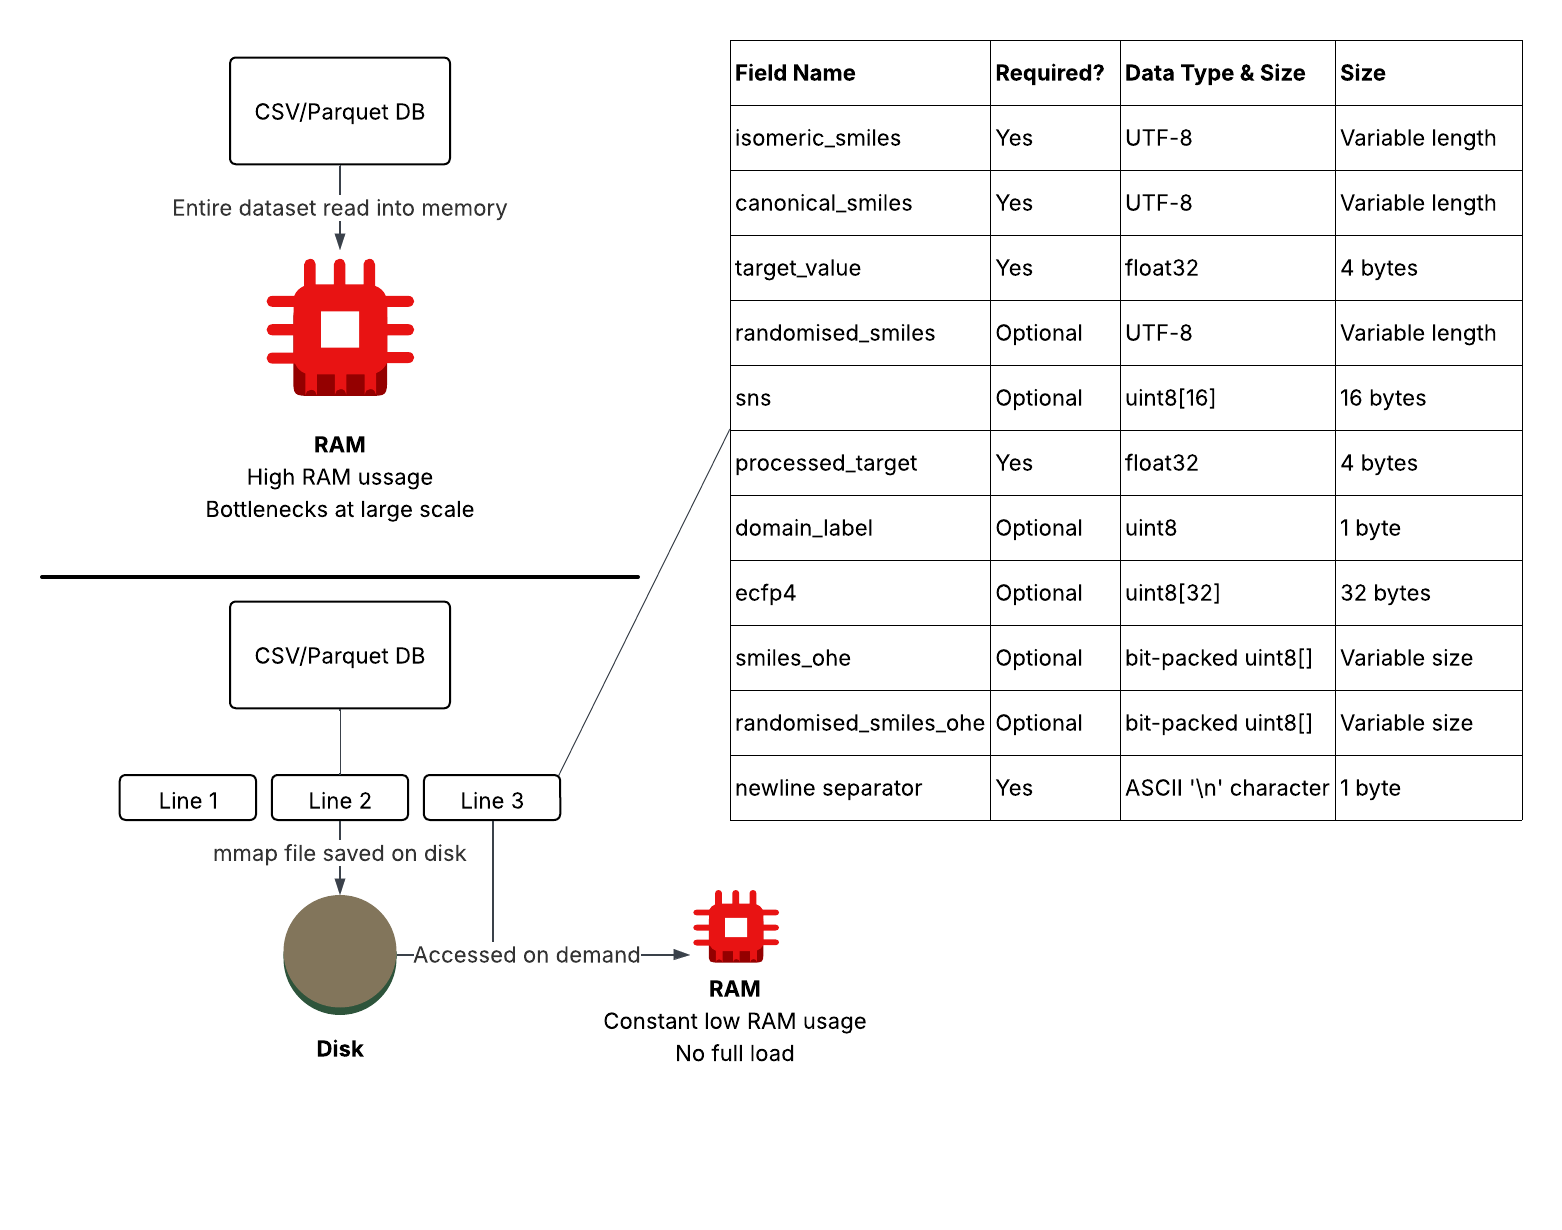
\includegraphics[width=0.95\textwidth,height=0.72\textheight,keepaspectratio]{figure_mmap_structure.png}
    \caption[In-memory and memory-mapped data loading.]{In-memory (top left) and memory-mapped (bottom left) data loading. Memory-mapped loading keeps each molecule as one record of a binary file on disk and reads records into memory on demand. The table on the right lists the fields of one record.}
    \label{fig:fig_mmap}
\end{figure}


\subsection{Uncertainty}
% [notes moved to thesis_notes_moved.md]

Up to this point we have been concerned with how noise affects the predictive performance of QSAR models. However, label noise should also affect the uncertainty these models report. Some models return only a point prediction, while others also return an estimate of uncertainty, either as a predicted distribution or as the spread across an ensemble. Furthermore, some report a single value of uncertainty while others report one that can be decomposed into an aleatoric and an epistemic component \citep{kendall2017}. The aleatoric component describes underlying noise the model associates with the data, while the epistemic component represents the uncertainty within the model's fit. We sought to determine if, as expected, the aleatoric component rises with injected label noise while the epistemic component does not.

For the BNN and VBLL transformations, we took the two components over $T = 100$ stochastic forward
passes \citep{kendall2017}:
\begin{equation}
\hat{u}^2_{\text{ale}}(x) = \frac{1}{T}\sum_{t=1}^{T}\hat{v}_t(x),
\qquad
\hat{u}^2_{\text{epi}}(x) = \frac{1}{T}\sum_{t=1}^{T}\big(\hat{\mu}_t(x) - \bar{\mu}(x)\big)^2 ,
\label{eq:sampling_split}
\end{equation}
where $\hat{\mu}_t(x)$ and $\hat{v}_t(x)$ are the mean and the variance returned for molecule $x$ on
pass $t$, and $\bar{\mu}(x)$ is the mean over passes. Here $\hat{v}_t(x)$ is the predicted observation
noise variance. It varies per molecule in the variance-head and heteroscedastic variants, and is one
number for the whole fit in the VBLL transformation. A full-BNN without a variance head returns no
variance, so its uncertainty is epistemic alone.

% TODO: review, needs manual review
The other models follow the same split. For GPs, the epistemic component is the posterior variance of the latent function and the aleatoric component is the learned observation noise \citep{Rasmussen2005}. Every GP except the heteroscedastic variant learns a single observation-noise variance for the whole fit, so its aleatoric component does not vary between molecules. For QRF models, each leaf holds several training molecules, and the aleatoric component for a molecule is the variance of the training labels in the leaf it falls into, averaged over the trees. The epistemic component is the variance of the leaf means across the trees. NGBoost predicts one variance for each molecule from a single fit, which is aleatoric alone \citep{Duan2020}. In every model, the total uncertainty is the sum of the aleatoric and epistemic components.

No held-out label carries injected noise, so every comparison against the injected noise was made on
training molecules. Each training set was divided into five folds grouped on Murcko scaffolds, and each
molecule was scored by a refit that excluded its own fold. For NGBoost on QM9, three of the five folds
were scored to limit its cost. No uncertainty was calibrated after fitting.


\subsection{Evaluation}
% [notes moved to thesis_notes_moved.md]
We computed statistics on the held-out molecules: for QM9 the test split, and for the three assay datasets the held-out fold of the scaffold cross-validation. Different combinations of dataset, model, representation, noise condition, and noise level are examined in each scenario. We used the coefficient of determination ($R^2$) throughout. For molecule $i$, let $y_i$ be the clean label, $\hat{y}_i$ the prediction, $\epsilon_i$ the noise injected into its label and $u_i$ the predicted uncertainty.

% TODO: review, needs manual review
To evaluate the effect of label noise, we tracked predictive performance retention under increasing artificial noise. For each QSAR pairing we recorded $R^2(x)$ at each noise level $x$, and normalized it to obtain the retention ratio $R^2(x)/R^2(0)$. To quantify robustness, we used the normalized area under this retention curve, \aucnorm{} (Equation~\ref{eq:auc_norm}), evaluated using the trapezoidal rule over the seven noise levels, $x \in \{0, 0.2, 0.3, 0.5, 0.75, 1.0, 1.5\}$, in the units of Equation~\ref{eq:dose_matching}. For censoring, the area is taken over the fractions of labels clipped, from 0 to 0.5, so its \aucnorm{} is not on the same axis as the other conditions.

An \aucnorm{} value near 1 indicates that the QSAR model in question has retained predictive performance with artificial noise, meaning it is more robust to noise. Since we normalize the curve by its own clean-label predictive performance, a model with a low clean $R^2$ has less to lose, so \aucnorm{} is reported beside clean $R^2$. We excluded every QM9 replicate or scaffold fold with a clean $R^2 < 0.3$ from the robustness analysis (Additional file~\ref{app:noise:sec:excluded_configurations}), as performance retention ratios become unstable when the clean-label denominator approaches zero. On QM9 one \aucnorm{} is computed per replicate, and we report the median over the 10 replicates. On the three assay datasets one value is computed per scaffold fold, and the median over the five folds is reported. 

% TODO: review, needs manual review
To test whether a model's robustness follows from its clean predictive performance, we computed Spearman's rank correlation ($\rho$) between clean $R^2$ and \aucnorm{} across the thirteen base models.

We conducted a separate analysis of variance (ANOVA) for each noise condition to identify the
relative contributions of molecular representation and model architecture to both predictive
performance and noise robustness. For a given metric $y$, either $R^2$ at a noise level of 1.0 (0.75 on Caco-2) or
\aucnorm:
\begin{equation}
y_{fmjr} = \mu + s_r + \alpha_f + \gamma_{m(f)} + \beta_j + (\alpha\beta)_{fj} + (\gamma\beta)_{m(f)j} + e_{fmjr},
\end{equation}
where $s_r$ represents the effect of replicate $r$, $\alpha_f$ represents the effect of model family $f$, $\gamma_{m(f)}$ represents the effect of model architecture $m$ within its family, $\beta_j$ represents the effect of
molecular representation $j$, $(\alpha\beta)_{fj}$ and $(\gamma\beta)_{m(f)j}$ are the interaction terms, and $e_{fmjr}$ is the
residual. The proportion of variance explained by each term was calculated as the
effect size
\begin{equation}
\eta^2_{\text{term}} = \frac{SS_{\text{term}}}{SS_{\text{total}}},
\end{equation}
using Type I (sequential) sums of squares, entered in the order replicate, model family, model architecture within family, molecular
representation, interaction. The 10 QM9 replicates provide the residual; on the three assay datasets the five scaffold folds take the place of the replicates. The uncertainty on each share is the 95\% interval of $\eta^2$ over 1,000 bootstrap resamples of whole replicates. These shares describe the models and representations tested here, not the choice of model or representation in general. 

ANOVA relies on the assumption that observations both within and across groups are independent. Two features of this study break that assumption. First, each QM9 replicate uses the same data split and the same noise draw for every model and representation, so observations from one replicate are not independent of each other; we therefore entered the replicate as a block. Second, across the whole set of models in this study, some pairs produced similar predictions that are not independent, so a method present in several near-identical versions would count several times toward the share of model architecture. To handle this issue, we grouped the models into families. We considered grouping pairs of models that share a method or an architecture, and compared each pair on clean $R^2$ and on \aucnorm{} under the three noise conditions run on every representation, separately on each of the six representations, which gives 24 comparisons per pair. A pair was grouped when the mean difference between the two models was smaller than their standard deviation across replicates in at least two thirds of these comparisons (Additional file~\ref{app:noise:sec:model_redundancy}). Five families met this criterion: RF with QRF (16 of 24), XGBoost with LightGBM (23 of 24), NN-$\alpha$ with BNN-$\alpha$ (20 of 24), NN-$\beta$ with BNN-$\beta$ (18 of 24), and VBLL-$\alpha$ with VBLL-$\beta$ (20 of 24). VBLL did not group with the plain or Bayesian network of its own architecture (4 to 10 of 24), as its clean $R^2$ was lower by 0.02 to 0.09, and NGBoost did not group with XGBoost or LightGBM (2 and 3 of 24). The two architectures of the plain networks, and of the Bayesian networks, also met the criterion (18 and 17 of 24); we grouped by architecture instead, which the evidence supports equally well. The thirteen base models therefore form eight families. Within these families, the differences between models accounted for at most 1.0\% of the variance in any outcome and noise condition on QM9, and up to 15.1\% of predictive performance on clean labels on the three assay datasets. We also ran Tukey's honestly significant difference test between the members of each family, separately for each representation (Additional file~\ref{app:noise:sec:tukey_within_families}). With 10 replicates it detects differences smaller than the variation between replicates, so we report it beside the size of each difference rather than use it to form the families.

% TODO: review, needs manual review
Across representations, we considered grouping Sort \& Slice with the ECFP4 fingerprint, as both encode overlapping circular substructure information. The grouping criterion held for none of the 13 base models on clean $R^2$, so all six representations were kept as separate levels (Additional file~\ref{app:noise:sec:representation_redundancy}).

% TODO: review, needs manual review
To assess the interaction between uncertainty estimation and label noise, we carried out four analyses. The first tested whether uncertainty rises with label noise, as measured by the mean $u_i$ over held-out molecules at the highest noise level
divided by its value with no added noise, in each fold. The second pertains to models that report separate aleatoric and epistemic components. We divided the increase of mean epistemic uncertainty between the highest level of noise and clean labels by the increase in the mean aleatoric component to determine how each responds to label noise. A ratio near 0 means the added noise was attributed to the labels while a ratio of 1 or above means the epistemic component grew as much or more. We also compared the mean aleatoric component with the standard deviation of the injected noise. The third tested whether per-sample uncertainty values track injected label noise, as measured by the Spearman correlation between $u_i$ and $|\epsilon_i|$ over out-of-fold training molecules, per fold and per noise level. We also report the Spearman correlation between $u_i$ and the absolute error of the prediction. The fourth tested whether dividing a molecule's out-of-fold absolute error by $u_i$ ranks the corrupted labels better than the error alone, and we report the difference between the two Spearman correlations with $|\epsilon_i|$.


\section{Variance Decomposition}
% [notes moved to thesis_notes_moved.md]

% TODO: review, needs manual review
Considering the two main components of a QSAR model, the molecular representation and the model architecture, we sought to understand how each contributes to both predictive performance and noise robustness. ANOVA decomposition divides the variance between model family, model architecture within its family, molecular representation, the pairing of the two, the replicate, and a residual. We ran this decomposition for Gaussian noise, the usual assumption, as well as the two conditions that act on scaffold families, grouped-wider and grouped-shifted (Figure~\ref{fig:variance}, Table~\ref{tab:variance}). For predictive performance measured in $R^2$ at a noise level of 1.0, model family and molecular representation account for comparable shares of the variance, 26.6\% and 29.0\% under Gaussian noise. However, for noise robustness, quantified by the normalized area under the $R^2$ retention curve (\aucnorm; higher values indicate greater robustness), model family accounts for 47.2\% of the variance while molecular representation accounts for 8.1\%. This pattern is observed across noise conditions. However, the interaction term between model architecture and molecular representation is slightly more influential with noise robustness than with predictive performance, 19.9\% against 14.2\%, though it is on par with the residual. Some models may depend on particular representations more strongly once the labels are noisy.

\begin{figure}[!htbp]
\centering
\includegraphics[width=\textwidth,height=0.72\textheight,keepaspectratio]{F2_variance_decomposition.png}
\caption[Variance decomposition of robustness and predictive performance on QM9.]{Share of the variance in each outcome explained by model family, model architecture within family, molecular representation, their pairing, the replicate, and the residual, on the QM9 HOMO--LUMO gap. a) Robustness, as \aucnorm; b) predictive performance, as $R^2$ at a noise level of 1.0, one spread of the clean training labels. The bottom axis is the noise condition, the side axis the share of variance. Whiskers are 95\% bootstrap intervals over replicates.}
\label{fig:variance}
\end{figure}

Comparing the decomposition before and after noise is added shows where model family matters (Table~\ref{tab:three_outcomes_qm9}, Figure~\ref{fig:three_outcomes}). For predictive performance, noise changes the division of the variance only a little. Representation explains about the same share of $R^2$ with and without noise, model family loses some of its share, and the replicate and the residual together take more. Robustness divides the variance differently. Representation explains 8.1\% of the variance in \aucnorm, against 31.1\% of clean $R^2$, while model family rises to 47.2\%. The replicate nearly disappears from \aucnorm, likely because each replicate's curve is divided by that replicate's own clean $R^2$, so a difficult split lowers both and cancels out.

\begin{table}[!htbp]
\centering
\small
\begin{adjustbox}{max width=\textwidth,max totalheight=0.78\textheight}
\begin{tabular}{lccc}
\toprule
Term & Clean $R^2$ & $R^2$ at noise level 1.0, Gaussian & \aucnorm, Gaussian \\
\midrule
Model family & 35.4 & 26.6 & 47.2 \\
Representation & 31.1 & 29.0 & 8.1 \\
Model $\times$ representation & 12.1 & 14.2 & 19.9 \\
Replicate & 10.6 & 13.4 & 1.7 \\
Residual & 10.2 & 16.0 & 22.6 \\
\bottomrule
\end{tabular}
\end{adjustbox}
\caption[Variance shares before and after Gaussian noise on QM9.]{Share of the variance (\%) in each outcome explained by each term, on the QM9 HOMO--LUMO gap, before and after Gaussian noise is added. Clean $R^2$ is predictive performance with no noise added; the second column is $R^2$ at the noise level named in its header; \aucnorm{} is robustness. Model within family, the remaining term, is left out, so a column does not sum to 100\%. Intervals are in Additional file~\ref{app:noise:sec:variance_intervals}. Values are over 10 replicates.}
\label{tab:three_outcomes_qm9}
\end{table}

% TODO: this figure shows the same numbers as Table tab:three_outcomes_qm9 (both are in the main text of the NoiseInject manuscript); keep one of the two if pages are short.
\begin{figure}[!htbp]
\centering
\includegraphics[width=\textwidth,height=0.72\textheight,keepaspectratio]{F2c_three_outcomes.png}
\caption[Variance shares of clean performance, noisy performance and robustness on QM9.]{Share of the variance in each outcome explained by each term on the QM9 HOMO--LUMO gap, in three groups: predictive performance on clean labels, predictive performance at a noise level of 1.0 under Gaussian noise, and robustness (\aucnorm) under Gaussian noise. One bar per term. Whiskers are 95\% intervals from 1,000 bootstrap resamples of whole replicates.}
\label{fig:three_outcomes}
\end{figure}

% TODO: review, needs manual review
Under grouped-shifted noise the pattern changes, because predictive performance varies widely between replicates, which gives the replicate a larger share. We find that 28.4\% of the variance in \aucnorm{} and 51.0\% of the variance in $R^2$ are due to the replicate, with model family falling to 32.7\% and 8.4\%. The offset applied to each scaffold family may therefore account for more of the variance in both $R^2$ and \aucnorm.

\begin{table}[!htbp]
\centering
\small
\begin{adjustbox}{max width=\textwidth,max totalheight=0.78\textheight}
\begin{tabular}{llcccccc}
\toprule
Condition & Outcome & Replicate $\eta^2$ (\%) & Model family $\eta^2$ (\%) & Model within family $\eta^2$ (\%) & Representation $\eta^2$ (\%) & Interaction $\eta^2$ (\%) & Residual $\eta^2$ (\%) \\
\midrule
None (clean labels) & Performance (clean $R^2$) & 10.6 & 35.4 & 0.6 & 31.1 & 12.1 & 10.2 \\
Gaussian & Robustness (\aucnorm) & 1.7 & 47.2 & 0.6 & 8.1 & 19.9 & 22.6 \\
Grouped-shifted & Robustness (\aucnorm) & 28.4 & 32.7 & 1.0 & 7.0 & 7.2 & 23.7 \\
Grouped-wider & Robustness (\aucnorm) & 1.7 & 46.3 & 0.3 & 7.9 & 18.5 & 25.3 \\
Gaussian & Performance ($R^2$ at level 1.0) & 13.4 & 26.6 & 0.8 & 29.0 & 14.2 & 16.0 \\
Grouped-shifted & Performance ($R^2$ at level 1.0) & 51.0 & 8.4 & 0.4 & 10.3 & 6.2 & 23.7 \\
Grouped-wider & Performance ($R^2$ at level 1.0) & 12.7 & 33.0 & 0.4 & 25.7 & 13.1 & 15.1 \\
\bottomrule
\end{tabular}
\end{adjustbox}
\caption[Variance decomposition by noise condition on QM9.]{Share of the variance in each outcome explained by the replicate, model family, model architecture within family, molecular representation, their pairing and the residual, on the QM9 HOMO--LUMO gap. Robustness is \aucnorm; performance is $R^2$ at a noise level of 1.0. Intervals are in Additional file~\ref{app:noise:sec:variance_intervals}. Thirteen base models in eight families by six representations, over 10 replicates.}
\label{tab:variance}
\end{table}

\section{Predictive Performance and Noise Robustness}
% [notes moved to thesis_notes_moved.md]

% TODO: review, needs manual review
The variance decomposition tells us what aspect of QSAR modeling affects predictive performance and robustness; however, it does not tell us about the characteristics of individual models. Every model's performance degrades as the labels get increasingly corrupted with noise (Figure~\ref{fig:curves}). Performance changes little until the artificial noise reaches about half the spread of the clean training labels, and then it begins to drop. The rate at which it drops and the amount of predictive performance retained are not necessarily correlated with the model's predictive performance on clean labels. Across the thirteen base models under Gaussian noise on ECFP4, clean $R^2$ and \aucnorm{} are unrelated, at a Spearman correlation of $-0.16$ ($p = 0.61$). If anything, the lower a model's predictive performance on clean labels, the less it has to lose as the labels get noisier.

\begin{figure}[!htbp]
\centering
\includegraphics[width=\textwidth,height=0.72\textheight,keepaspectratio]{F4a_models_under_noise.png}
\caption[Predictive performance against Gaussian label noise on QM9.]{Predictive performance against label noise on the QM9 HOMO--LUMO gap under Gaussian noise, for the eight base models with the highest \aucnorm{} on ECFP4. a) ECFP4; b) PDV, drawn for the same eight models. Bottom axis: the noise level, as a fraction of the spread of the clean training labels. Side axis: $R^2$ on held-out molecules, as the median over 10 replicates. The dashed vertical line marks the noise level of 1.0 at which $R^2$ is reported.}
\label{fig:curves}
\end{figure}

The link between predictive performance and noise robustness can be examined by model family (Figure~\ref{fig:decoupling}, Table~\ref{tab:robustness}). The forests, XGBoost, LightGBM, SVM and GP all retain relatively high predictive performance on clean labels while maintaining relatively strong robustness to noise. NN-$\beta$ and BNN-$\beta$ are among the highest in predictive performance on clean labels, and the four plain and Bayesian networks are the four least robust. The two variational networks sit between these groups, with lower predictive performance on clean labels and middling noise robustness. Standard feed-forward networks can make strong predictions under clean labels; however, they are not a safe bet under noisy ones.

\begin{figure}[!htbp]
\centering
\includegraphics[width=\textwidth,height=0.72\textheight,keepaspectratio]{R16_decoupling_ecfp4.png}
\caption[Clean predictive performance against robustness on QM9.]{Predictive performance on clean labels against robustness, on the QM9 HOMO--LUMO gap on ECFP4, under a) Gaussian and b) grouped-shifted noise. One point per base model. Bottom axis: $R^2$ with no noise added to the training labels. Side axis: \aucnorm, on one scale across both panels. Because \aucnorm{} divides by clean $R^2$, a model with a low clean $R^2$ has less to lose.}
\label{fig:decoupling}
\end{figure}

% TODO: the four plain and Bayesian networks' grouped columns and clean R^2 will move once their clean scores are fixed (carried over from the NoiseInject manuscript).
\begin{table}[!htbp]
\centering
\small
\begin{adjustbox}{max width=\textwidth,max totalheight=0.78\textheight}
\begin{tabular}{lcccccccc}
\toprule
Model & Clean $R^2$ & Gaussian & Grouped-wider & Grouped-shifted & Censoring & Student-$t$ ($\nu$=5) & Outlier (10\%) & Laplace \\
\midrule
RF & 0.832 & 0.963 & 0.967 & 0.937 & 0.817 & 0.966 & 0.969 & 0.967 \\
QRF & 0.830 & 0.956 & 0.973 & 0.928 & --- & --- & --- & --- \\
XGBoost & 0.835 & 0.946 & 0.940 & 0.918 & --- & --- & --- & --- \\
LightGBM & 0.845 & 0.938 & 0.937 & 0.908 & --- & --- & --- & --- \\
NGBoost & 0.706 & 0.979 & 0.953 & 0.933 & --- & 0.969 & 0.963 & 0.966 \\
SVM & 0.844 & 0.937 & 0.955 & 0.908 & --- & 0.945 & 0.951 & 0.951 \\
GP & 0.839 & 0.938 & 0.939 & 0.905 & --- & 0.940 & 0.938 & 0.936 \\
NN-$\alpha$ & 0.794 & 0.910 & 0.910 & 0.857 & --- & --- & --- & --- \\
BNN-$\alpha$ & 0.820 & 0.887 & 0.886 & 0.853 & --- & --- & --- & --- \\
VBLL-$\alpha$ & 0.772 & 0.926 & 0.927 & 0.920 & --- & --- & --- & --- \\
NN-$\beta$ & 0.842 & 0.872 & 0.881 & 0.848 & --- & --- & --- & --- \\
BNN-$\beta$ & 0.839 & 0.871 & 0.866 & 0.840 & --- & --- & --- & --- \\
VBLL-$\beta$ & 0.754 & 0.924 & 0.925 & 0.916 & --- & --- & --- & --- \\
\bottomrule
\end{tabular}
\end{adjustbox}
% TODO: review, needs manual review
% TODO: model lists in this caption are taken from qsar_qm_models/deep_run_pairs.json and censoring_pairs.json (the run configuration), not from the result files; confirm every listed pairing ran.
\caption[Robustness of each base model under each noise condition on QM9.]{Robustness (\aucnorm) of each base model under each noise condition on the QM9 HOMO--LUMO gap with ECFP4, with clean $R^2$ in the first column. A dash is a pairing the condition was not run on. Laplace, Student-$t$ and outlier noise were run on eight models, RF, NGBoost, SVM, the GP, GP (het.), BNN-$\alpha$ (var.\ head), VBLL-$\alpha$ (het.) and VBLL-$\beta$ (het.), on ECFP4, PDV and ChemBERTa. Censoring was run on five pairings, RF and GP (het.) on ECFP4 and NGBoost, the GP and BNN-$\alpha$ (var.\ head) on PDV. Values are medians over 10 replicates.}
\label{tab:robustness}
\end{table}

% TODO: review, needs manual review
NGBoost is a standout case in the sense that it is highly dependent on its paired molecular representation. Under Gaussian noise it has the highest \aucnorm{} on every one of the six representations, yet also the lowest predictive performance on clean labels on four of the six representations. Its high robustness is partly due to the fact that a model that starts from low predictive performance does not have as much to lose. It also maintains shallow robustness curves across representations. On ECFP4, NGBoost's predictive performance ranks lowest up to a noise level of 0.75 and stays in the lower half at every noise level. However, on PDV it starts second lowest and ends highest, surpassing the other models between noise levels 1.0 and 1.5. So when paired with the right features, NGBoost has the potential to make better predictions under higher quantities of label noise. Under grouped-shifted noise, RF has higher \aucnorm{} values than NGBoost on ECFP4, Avalon and ChemBERTa. Even then, NGBoost reports the highest noise robustness for PDV, MHG-GNN and Sort \& Slice. While NGBoost on PDV performs well under higher label noise, LightGBM performs well under smaller quantities of noise. Its performance drops sharply after a noise level of 1.0.

% TODO: review, needs manual review
The choice of representation can affect noise robustness, but how much depends on the model family (Figure~\ref{fig:grid}). All of the neural networks span a wider range of \aucnorm{} across the six representations than any of the other models, 0.037 to 0.069 against at most 0.030. Between ECFP4 and PDV under Gaussian noise, the four plain and Bayesian networks differ by between 0.037 and 0.065 of \aucnorm, while no tree or kernel model shifts by more than 0.011. This does not hold for every network; the two variational networks move by 0.009 and 0.019. So while molecular representation is not the primary factor in what makes a model robust to noise, the choice of which molecular representation to use matters with certain models, particularly neural networks.

\begin{figure}[!htbp]
\centering
\includegraphics[width=\textwidth,height=0.72\textheight,keepaspectratio]{F3_model_by_representation.png}
\caption[Robustness of each base model on each representation on QM9.]{Robustness (\aucnorm) of the thirteen base models on the QM9 HOMO--LUMO gap under a) Gaussian and b) grouped-shifted noise. Rows are models, ordered by family, and columns the six representations. Color is fixed across both panels, its bright end the higher \aucnorm. Values are medians over 10 replicates; excluded configurations are listed in Additional file~\ref{app:noise:sec:excluded_configurations}, and the grid under grouped-wider noise is in Additional file~\ref{app:noise:sec:grouped_wider_grid}.}
\label{fig:grid}
\end{figure}

\section{Artificial Noise Conditions}
% [notes moved to thesis_notes_moved.md]

% TODO: review, needs manual review
Many studies involving experimental label noise rely on the assumption that noise can be modeled by a Gaussian distribution. We decided to vary the distribution from which noise is drawn, as well as the way in which it is injected into specific labels. Five of the seven conditions draw each label's error on its own, so the error is random. Grouped-shifted gives a whole scaffold family a shared offset, and censoring pulls every label above a limit down to that limit, so in both the error is systematic. Every condition except censoring adds the same expected amount of noise at a given noise level (Section~\ref{sec:noise_injection}), so a difference between two conditions is a difference in pattern rather than amount. Censoring could not be held to a set amount, as its levels count the fraction of labels clipped.

We compare Gaussian noise on the HOMO--LUMO gap to Laplace, Student-$t$ and outlier noise in Figure~\ref{fig:deep}. The shape of the distribution from which the noise was drawn made little difference. SVM reported higher \aucnorm{} values on non-Gaussian label noise, 0.937 under Gaussian noise against 0.947, 0.952 and 0.955 under Student-$t$, outlier and Laplace noise on PDV (the ECFP4 values are in Table~\ref{tab:robustness}), while NGBoost lost \aucnorm{} under every one. NGBoost's relatively stronger performance under Gaussian noise makes sense, as it fits a per-molecule scale under a Gaussian likelihood, which the other distributions violate. No single change exceeds the spread across that pairing's ten replicates on QM9. These results coincide with \citet{Heid2023}, who found no difference between error distributions drawn at a matched mean and standard deviation.

\begin{figure}[!htbp]
\centering
\includegraphics[width=\textwidth,height=0.72\textheight,keepaspectratio]{R19_deep_conditions_qm9.png}
% TODO: review, needs manual review
\caption[Robustness under every noise condition on a subset of models on QM9.]{Robustness (\aucnorm) under the noise conditions run on the eight models and three representations listed under Table~\ref{tab:robustness}, on the QM9 HOMO--LUMO gap. a) ECFP4; b) PDV; c) ChemBERTa. Rows are models and columns noise conditions, with Gaussian on the left. Values are medians over 10 replicates, on one color scale across all panels. Censoring is shown here rather than on the curves because its level is a fraction of labels clipped; its \aucnorm{} is an area over a different quantity from the columns beside it. A gray square marks a pairing that was not run.}
\label{fig:deep}
\end{figure}

% TODO: review, needs manual review
The Gaussian distribution stands in well for the other noise shapes, but not for systematic noise. Relative to Gaussian, grouped-shifted noise lowered \aucnorm{} across all models and representations (Table~\ref{tab:condition_cost}). The models struggle when the molecules of a scaffold family share an offset rather than each receiving an independent error. For RF on ECFP4, the grouped-shifted curve separates from those of the other conditions from a noise level of 0.75 (Figure~\ref{fig:conditions}). The variational networks retained the most predictive performance, while the plain, deterministic NNs lost the most. BNN-$\alpha$ lost less \aucnorm{} between Gaussian and grouped-shifted noise than NN-$\alpha$ on every representation except PDV, while BNN-$\beta$ lost less than NN-$\beta$ by more than 0.01 only on MHG-GNN and PDV (Table~\ref{tab:condition_cost}). Grouped-wider noise changed no model beyond its replicate spread except QRF on Avalon and MHG-GNN, whose \aucnorm{} rose under this condition. Censoring gave \aucnorm{} values 0.12 to 0.18 below those under Gaussian noise for the same models, although its noise level counts the fraction of labels clipped and so is not the same axis (Figure~\ref{fig:deep}).

\begin{table}[!htbp]
\centering
\small
\begin{adjustbox}{max width=\textwidth,max totalheight=0.78\textheight}
\begin{tabular}{lcccccccc}
\toprule
Model & ECFP4 & PDV & MHG-GNN & Avalon & ChemBERTa & Sort \& Slice & Replicate spread & Beats it on \\
\midrule
RF & -0.025 & -0.024 & -0.025 & -0.038 & -0.025 & -0.028 & 0.013--0.022 & 6 of 6 \\
QRF & -0.027 & -0.027 & -0.032 & -0.042 & -0.027 & -0.038 & 0.016--0.031 & 5 of 6 \\
XGBoost & -0.028 & -0.039 & -0.035 & -0.052 & -0.030 & -0.025 & 0.016--0.039 & 5 of 6 \\
LightGBM & -0.030 & -0.037 & -0.037 & -0.058 & -0.028 & -0.037 & 0.016--0.033 & 5 of 6 \\
NGBoost & -0.046 & -0.030 & -0.039 & -0.062 & -0.041 & -0.039 & 0.019--0.041 & 6 of 6 \\
SVM & -0.029 & -0.045 & -0.034 & -0.053 & -0.040 & -0.038 & 0.022--0.043 & 5 of 6 \\
GP & -0.034 & -0.048 & -0.040 & -0.054 & -0.045 & -0.041 & 0.025--0.038 & 6 of 6 \\
NN-$\alpha$ & -0.053 & -0.051 & -0.060 & -0.115 & -0.044 & -0.053 & 0.025--0.055 & 4 of 6 \\
BNN-$\alpha$ & -0.034 & -0.053 & -0.034 & -0.073 & -0.039 & -0.025 & 0.027--0.075 & 2 of 6 \\
VBLL-$\alpha$ & -0.006 & -0.014 & -0.020 & -0.005 & -0.007 & -0.013 & 0.029--0.047 & 0 of 6 \\
NN-$\beta$ & -0.024 & -0.080 & -0.052 & -0.076 & -0.047 & -0.045 & 0.032--0.048 & 4 of 6 \\
BNN-$\beta$ & -0.030 & -0.050 & -0.019 & -0.075 & -0.055 & -0.041 & 0.032--0.180 & 2 of 6 \\
VBLL-$\beta$ & -0.007 & -0.028 & -0.033 & -0.010 & -0.028 & -0.009 & 0.030--0.066 & 0 of 6 \\
\bottomrule
\end{tabular}
\end{adjustbox}
\caption[Change in robustness from Gaussian to grouped-shifted noise on QM9.]{The change in \aucnorm{} from Gaussian to grouped-shifted noise on the QM9 HOMO--LUMO gap, for each base model on each representation; negative is a loss. The replicate spread is the highest minus the lowest \aucnorm{} across a pairing's 10 replicates under Gaussian noise, given as its range over the representations. The last column counts the representations on which the loss exceeds that spread.}
\label{tab:condition_cost}
\end{table}

\begin{figure}[!htbp]
\centering
\includegraphics[width=\textwidth,height=0.72\textheight,keepaspectratio]{F4b_rf_across_noise_conditions.png}
\caption[Random forest under each noise condition on QM9.]{Predictive performance of the random forest under each noise condition, one line per condition, on the QM9 HOMO--LUMO gap on ECFP4. The bottom axis is the noise added to the training labels, as a fraction of their clean spread, and the side axis median held-out $R^2$ over 10 replicates. Grouped-shifted is the line that separates from the rest, visibly from a level of 0.75. Censoring has no line, as it cannot share this bottom axis.}
\label{fig:conditions}
\end{figure}

% TODO: review, needs manual review
While we established that the choice of representation has only a minor impact on noise robustness, representations do seem to perform better or worse under different noise conditions. When compared to Gaussian noise, under grouped-shifted noise NGBoost went from performing best on Avalon to PDV, SVM went from ChemBERTa to ECFP4 and BNN-$\alpha$ from PDV to MHG-GNN. There is no single best representation for \aucnorm; rather, it depends on the underlying data, including both the samples themselves and the underlying label noise. A representation chosen under one assumption about the noise is therefore not necessarily the best under another.

Most of these observations are made at the upper end of the noise range. With ECFP4, six of the seven most robust models start within 0.015 of one another in $R^2$ for clean labels, stay together up to a noise level of 0.5 and separate only above 1.0, finishing between 0.692 for LightGBM and 0.741 for RF (Figure~\ref{fig:curves}). We ranked the models by predictive performance at each noise level. Of the thirteen base models, RF started ranked seventh, but by level 1.0 it was ranked first. SVM, on the other hand, falls from first to fifth (Figure~\ref{fig:rank_level}). Because \aucnorm{} weights the whole range from 0 to 1.5 equally, and the first half of it separates little, it has the potential to understate just how much the pattern of the noise costs. However, choosing to look at performance at a set level has its drawbacks, as the ranks shift at a different pace between noise conditions.

\begin{figure}[!htbp]
\centering
\includegraphics[width=\textwidth,height=0.36\textheight,keepaspectratio]{R15_rank_against_level_ecfp4_gaussian.png}\\[4pt]
\includegraphics[width=\textwidth,height=0.36\textheight,keepaspectratio]{R15_rank_against_level_ecfp4_grouped_shifted.png}
\caption[Rank of each base model at each noise level on QM9.]{Rank of each base model for predictive performance at each noise level, on the QM9 HOMO--LUMO gap on ECFP4, under a) Gaussian and b) grouped-shifted noise. The bottom axis is the noise level and the side axis the rank among the thirteen base models, 1 the highest predictive performance. Models are ranked within each replicate and the median rank is drawn, so tied medians appear as half ranks.}
\label{fig:rank_level}
\end{figure}

\section{Robustness on the Three Assay Datasets}
% [notes moved to thesis_notes_moved.md]

% TODO: review, needs manual review
So far, we have only discussed results on the HOMO--LUMO gap from QM9, a computed property whose labels carry negligible measurement noise. We repeated these experiments on three experimentally obtained datasets, LogD, Caco-2 \citep{openadmet} and hERG $K_i$ \citep{Zdrazil2023}, replicating our process of adding artificial noise. Unlike QM9, the experimental endpoints carry their own measurement noise in both training and test labels; the injected artificial noise therefore adds on top of an unknown noise floor. Repeat measurements of the same compound disagree by about 0.54 log units for p$K_i$ \citep{Kalliokoski2013, Kramer2012}. The hERG $K_i$ labels have a spread of 0.915 log units, so a noise level of 0.6 of that spread is about one unit of that estimated laboratory error. Each model's \aucnorm{} under the three noise conditions run on every model is given with its clean $R^2$ beside it (Figure~\ref{fig:assay}).

% TODO: review, needs manual review
Tables~\ref{tab:three_outcomes_logd}, \ref{tab:three_outcomes_caco2} and~\ref{tab:three_outcomes_herg} repeat the QM9 comparison on the three assay datasets, and Figure~\ref{fig:variance_clean} and Table~\ref{tab:variance_clean} give the clean decomposition on all four. On every dataset, representation explains about the same share of predictive performance with and without noise and a smaller share of robustness than of predictive performance, while model family explains the largest share of robustness. Noise raises the share of the replicate and the residual in predictive performance on every dataset. On Caco-2 and hERG $K_i$ the replicate, which on these datasets is one of five scaffold folds, is the largest share of predictive performance before and after noise is added, but falls well below model family for robustness. Across Gaussian, grouped-wider and grouped-shifted noise on all four datasets, representation explains at most 11.2\% of the variance in \aucnorm{}, on LogD under grouped-shifted noise (Additional file~\ref{app:noise:sec:variance_intervals}).

\begin{table}[!htbp]
\centering
\small
\begin{adjustbox}{max width=\textwidth,max totalheight=0.78\textheight}
\begin{tabular}{lccc}
\toprule
Term & Clean $R^2$ & $R^2$ at noise level 1.0, Gaussian & \aucnorm, Gaussian \\
\midrule
Model family & 60.2 & 59.6 & 58.0 \\
Representation & 16.8 & 14.8 & 7.1 \\
Model $\times$ representation & 9.5 & 9.3 & 12.2 \\
Replicate & 3.3 & 4.5 & 1.3 \\
Residual & 3.6 & 6.3 & 16.3 \\
\bottomrule
\end{tabular}
\end{adjustbox}
\caption[Variance shares before and after Gaussian noise on LogD.]{Share of the variance (\%) in each outcome explained by each term, on LogD, before and after Gaussian noise is added. Clean $R^2$ is predictive performance with no noise added; the second column is $R^2$ at the noise level named in its header; \aucnorm{} is robustness. Model within family, the remaining term, is left out, so a column does not sum to 100\%. Intervals are in Additional file~\ref{app:noise:sec:variance_intervals}. Values are over five scaffold folds. No fold fell below the clean $R^2$ threshold of 0.3, so all three columns use the same fits.}
\label{tab:three_outcomes_logd}
\end{table}

\begin{table}[!htbp]
\centering
\small
\begin{adjustbox}{max width=\textwidth,max totalheight=0.78\textheight}
\begin{tabular}{lccc}
\toprule
Term & Clean $R^2$ & $R^2$ at noise level 0.75, Gaussian & \aucnorm, Gaussian \\
\midrule
Model family & 22.8 & 11.4 & 43.2 \\
Representation & 9.9 & 9.7 & 3.1 \\
Model $\times$ representation & 8.9 & 6.6 & 9.4 \\
Replicate & 38.7 & 56.0 & 18.6 \\
Residual & 6.2 & 10.5 & 20.8 \\
\bottomrule
\end{tabular}
\end{adjustbox}
\caption[Variance shares before and after Gaussian noise on Caco-2.]{Share of the variance (\%) in each outcome explained by each term, on Caco-2, before and after Gaussian noise is added. Clean $R^2$ is predictive performance with no noise added; the second column is $R^2$ at the noise level named in its header; \aucnorm{} is robustness. Model within family, the remaining term, is left out, so a column does not sum to 100\%. Intervals are in Additional file~\ref{app:noise:sec:variance_intervals}. Values are over five scaffold folds. Predictive performance under noise is reported at a noise level of 0.75 on Caco-2 rather than 1.0, because its clean $R^2$ is the lowest of the four datasets and leaves the models less predictive performance to lose. The \aucnorm{} column excludes scaffold folds whose clean $R^2$ was below 0.3 (58 of 390 under Gaussian noise, mostly the Bayesian and VBLL networks on ChemBERTa and MHG-GNN); the two $R^2$ columns include every fold.}
\label{tab:three_outcomes_caco2}
\end{table}

\begin{table}[!htbp]
\centering
\small
\begin{adjustbox}{max width=\textwidth,max totalheight=0.78\textheight}
\begin{tabular}{lccc}
\toprule
Term & Clean $R^2$ & $R^2$ at noise level 1.0, Gaussian & \aucnorm, Gaussian \\
\midrule
Model family & 18.4 & 22.5 & 47.9 \\
Representation & 6.7 & 5.6 & 0.8 \\
Model $\times$ representation & 14.3 & 7.0 & 13.0 \\
Replicate & 28.1 & 39.4 & 5.0 \\
Residual & 17.5 & 23.5 & 28.0 \\
\bottomrule
\end{tabular}
\end{adjustbox}
\caption[Variance shares before and after Gaussian noise on hERG $K_i$.]{Share of the variance (\%) in each outcome explained by each term, on hERG $K_i$, before and after Gaussian noise is added. Clean $R^2$ is predictive performance with no noise added; the second column is $R^2$ at the noise level named in its header; \aucnorm{} is robustness. Model within family, the remaining term, is left out, so a column does not sum to 100\%. Intervals are in Additional file~\ref{app:noise:sec:variance_intervals}. Values are over five scaffold folds. The \aucnorm{} column excludes scaffold folds whose clean $R^2$ was below 0.3 (35 of 390 under Gaussian noise, mostly the Bayesian and VBLL networks); the two $R^2$ columns include every fold.}
\label{tab:three_outcomes_herg}
\end{table}

\begin{figure}[!htbp]
\centering
\includegraphics[width=\textwidth,height=0.72\textheight,keepaspectratio]{F2b_clean_decomposition.png}
\caption[Variance decomposition of clean predictive performance on all four datasets.]{Share of the variance in predictive performance on clean labels explained by model family, model architecture within family, molecular representation, their pairing, the replicate, and the residual, on all four datasets. Predictive performance is $R^2$ on held-out molecules with no noise added to the training labels. The bottom axis is the dataset, the side axis the share of variance; the six shares within a dataset sum to 100\%. There is no noise-condition axis: the clean fit is made once per replicate and every noise condition starts from it. Whiskers are 95\% bootstrap intervals over replicates; on each assay dataset a replicate is one of five scaffold folds. Thirteen base models in eight families by six representations, 10 replicates on QM9 and five on each assay dataset.}
\label{fig:variance_clean}
\end{figure}

\begin{table}[!htbp]
\centering
\small
\begin{adjustbox}{max width=\textwidth,max totalheight=0.78\textheight}
\begin{tabular}{lcccccc}
\toprule
Dataset & Replicate $\eta^2$ (\%) & Model family $\eta^2$ (\%) & Model within family $\eta^2$ (\%) & Representation $\eta^2$ (\%) & Interaction $\eta^2$ (\%) & Residual $\eta^2$ (\%) \\
\midrule
Caco-2 & 38.7 & 22.8 & 13.4 & 9.9 & 8.9 & 6.2 \\
hERG $K_i$ & 28.1 & 18.4 & 15.1 & 6.7 & 14.3 & 17.5 \\
LogD & 3.3 & 60.2 & 6.7 & 16.8 & 9.5 & 3.6 \\
QM9 (HOMO--LUMO gap) & 10.6 & 35.4 & 0.6 & 31.1 & 12.1 & 10.2 \\
\bottomrule
\end{tabular}
\end{adjustbox}
\caption[Variance decomposition of clean predictive performance by dataset.]{Share of the variance in predictive performance on clean labels explained by the replicate, model family, model architecture within family, molecular representation, their pairing and the residual, one row per dataset. The HOMO--LUMO gap row is the same decomposition as the first row of Table~\ref{tab:variance}. Intervals are in Additional file~\ref{app:noise:sec:variance_intervals}. On each assay dataset a replicate is one of five scaffold folds. Thirteen base models in eight families by six representations, over 10 replicates on QM9 and five on each assay dataset.}
\label{tab:variance_clean}
\end{table}

% TODO: review, needs manual review
As on QM9, the noise distribution changes the \aucnorm{} of most models little (Table~\ref{tab:assay_shape}). Laplace, Student-$t$ and outlier noise were run on seven models, RF, the two GPs, SVM, NGBoost, BNN-$\alpha$ (var.\ head) and VBLL-$\beta$ (het.), on ECFP4, PDV and ChemBERTa. Each change below is measured from the same model's \aucnorm{} under Gaussian noise. RF and the two GPs never lose more than 0.03 of \aucnorm{} under these three conditions or under grouped-wider noise, on any dataset or representation. SVM and NGBoost again move in opposite directions: SVM never loses \aucnorm{} under any of the four, while NGBoost loses under all four on Caco-2 and hERG $K_i$. The two networks move in both directions, by up to 0.110.

\begin{table}[!htbp]
\centering
\small
\begin{adjustbox}{max width=\textwidth,max totalheight=0.78\textheight}
\begin{tabular}{llccccc}
\toprule
Dataset & Model & Gaussian & Laplace & Student-$t$ ($\nu$=5) & Outlier (10\%) & Grouped-wider \\
\midrule
LogD & RF & 0.935 & +0.018 & +0.006 & +0.007 & +0.021 \\
LogD & GP & 0.891 & +0.004 & +0.003 & -0.001 & +0.006 \\
LogD & GP (het.) & 0.896 & 0.000 & -0.002 & -0.007 & -0.003 \\
LogD & SVM & 0.879 & +0.044 & +0.023 & +0.027 & +0.044 \\
LogD & NGBoost & 0.924 & 0.000 & -0.028 & -0.032 & -0.009 \\
LogD & BNN-$\alpha$ (var.\ head) & 0.881 & -0.013 & -0.013 & -0.024 & -0.029 \\
LogD & VBLL-$\beta$ (het.) & 0.796 & +0.010 & +0.012 & +0.020 & +0.068 \\
Caco-2 & RF & 0.865 & +0.035 & +0.028 & +0.026 & +0.053 \\
Caco-2 & GP & 0.809 & +0.039 & +0.034 & +0.020 & +0.023 \\
Caco-2 & GP (het.) & 0.815 & +0.035 & +0.032 & +0.011 & +0.019 \\
Caco-2 & SVM & 0.841 & +0.049 & +0.051 & +0.031 & +0.018 \\
Caco-2 & NGBoost & 0.878 & -0.069 & -0.038 & -0.060 & -0.147 \\
Caco-2 & BNN-$\alpha$ (var.\ head) & 0.787 & -0.110 & +0.092 & -0.043 & -0.017 \\
Caco-2 & VBLL-$\beta$ (het.) & 0.707 & +0.036 & +0.025 & +0.015 & +0.032 \\
hERG $K_i$ & RF & 0.898 & +0.015 & -0.006 & +0.016 & -0.012 \\
hERG $K_i$ & GP & 0.831 & +0.022 & +0.034 & +0.025 & +0.030 \\
hERG $K_i$ & GP (het.) & 0.843 & +0.010 & +0.036 & +0.015 & +0.021 \\
hERG $K_i$ & SVM & 0.859 & +0.051 & +0.035 & +0.025 & +0.055 \\
hERG $K_i$ & NGBoost & 0.842 & -0.031 & -0.027 & -0.042 & -0.093 \\
hERG $K_i$ & BNN-$\alpha$ (var.\ head) & 0.809 & -0.034 & -0.032 & -0.063 & -0.009 \\
hERG $K_i$ & VBLL-$\beta$ (het.) & 0.836 & +0.007 & -0.047 & +0.005 & -0.002 \\
\bottomrule
\end{tabular}
\end{adjustbox}
% TODO: review, needs manual review
\caption[Robustness under the noise distributions on the three assay datasets.]{Robustness under the noise distributions run on seven models, the rows of this table, on the three assay datasets, ECFP4. One row is one model on one dataset. The first column is \aucnorm{} under Gaussian noise; the others are the change in \aucnorm{} from it under each condition, negative a loss. Values are medians over five scaffold folds.}
\label{tab:assay_shape}
\end{table}

% TODO: review, needs manual review
Of the three conditions run on every model, grouped-shifted noise is the hardest on every dataset: it gave the lowest \aucnorm{} for nearly every model and representation, the main exceptions being the two VBLL networks on LogD and Caco-2. Under this condition RF is the most robust model on hERG $K_i$ and LogD and has the highest predictive performance on hERG $K_i$.

LightGBM has particularly varied results across the datasets. On LogD, it has relatively high predictive performance and middle-of-the-pack noise robustness. However, on hERG $K_i$ and Caco-2, it loses the most with increased noise, particularly under Gaussian and grouped-shifted noise. The effects are not as pronounced under grouped-wider noise, although it still ranks among the least robust there. XGBoost degrades in the same way on hERG $K_i$ and Caco-2.

% TODO: ranks in this paragraph are among the 13 base models; Figure fig:transfer ranks 19. A re-ranking of the 13 from results/decisions/auc_norm_*.csv (median AUC_norm, Gaussian) gave RF up to 8th (Caco-2, Sort & Slice) and 2nd on QM9 at all six representations, against "first and seventh" and "second or third" here; unverified whether the text used per-replicate ranks. Re-check, or redraw the figure on 13.
% TODO: review, needs manual review
While the performance is not identical between the datasets, some rankings hold across them (Figure~\ref{fig:transfer}, which ranks all 19 models; the ranks below are among the thirteen base models). RF is the most consistent: among the thirteen base models under Gaussian noise it ranks between first and seventh for \aucnorm{} on every dataset and representation, second or third on QM9 and first on LogD at five of six. The GP has the highest predictive performance on clean labels on all three assay datasets with nearly every representation, and ranks third to ninth for \aucnorm. NGBoost, the most robust model on QM9, ranks first to third on LogD, second to tenth on Caco-2 and sixth to ninth on hERG $K_i$. LightGBM falls furthest, ranking 10th to 13th on Caco-2 and hERG $K_i$ at every representation while being among the highest in predictive performance on clean labels. VBLL-$\alpha$ is the opposite, ranking first or second for \aucnorm{} on hERG $K_i$ and last on LogD at every representation, from one of the lowest clean $R^2$ values. Its robustness depends on the dataset rather than on the representation.

% TODO: review, needs manual review
Across the four datasets, the base models fall into two groups (Table~\ref{tab:leaders}). The forests, RF and QRF, are reliably robust. They rank among the most robust base models on every dataset under each noise condition run on all models, with Caco-2 under grouped-shifted noise the weakest case. They also lead predictive performance under grouped-shifted noise on QM9 and hERG $K_i$, although their predictive performance on clean labels is middling. The other models perform well only under some conditions, and several of them are where the interaction between model and representation in the variance decomposition comes from. The GP has the highest or close to the highest predictive performance on clean labels and under Gaussian noise on every assay dataset, and changes little with representation, but under grouped-shifted noise it matches the leading model only on LogD. Its \aucnorm{} is middling because it starts from the highest $R^2$ and has the most to lose. NGBoost is among the most robust models on QM9 and LogD, but it predicts well only with the right representation, such as PDV. SVM is middling for robustness but leads for predictive performance under grouped-shifted noise on LogD and under grouped-wider noise on hERG $K_i$. The plain and Bayesian networks have high predictive performance on clean labels, are the least robust, and depend most on representation. The VBLL networks are among the most robust on Caco-2 and hERG $K_i$, from low predictive performance on clean labels, and the least robust on LogD. LightGBM and XGBoost combine high predictive performance on clean labels with some of the lowest robustness on Caco-2 and hERG $K_i$. How much noise is expected matters as well. At a noise level of 0.5 the models still rank by predictive performance much as they do on clean labels, while by 1.0 the order has changed, most of all on Caco-2 and hERG $K_i$. The order of models by \aucnorm{} is broadly similar across noise conditions, with the forests near the top under each. On every dataset the leading pairings in the table are closer together than their range over replicates, so each row names a group of near-equivalent choices.

\begin{table}[!htbp]
\centering
\small
\begin{adjustbox}{max width=\textwidth,max totalheight=0.78\textheight}
\begin{tabular}{llllccllc}
\toprule
Dataset & Labels & Leading model & Representation & $R^2$ & Range & Second model & Representation & $R^2$ \\
\midrule
QM9 & Clean labels & NN-$\alpha$ & PDV & 0.911 & 0.069 & NN-$\beta$ & PDV & 0.909 \\
QM9 & Gaussian & LightGBM & Sort \& Slice & 0.845 & 0.054 & NN-$\alpha$ & PDV & 0.840 \\
QM9 & Grouped-wider & QRF & PDV & 0.852 & 0.033 & QRF & MHG-GNN & 0.850 \\
QM9 & Grouped-shifted & RF & PDV & 0.816 & 0.249 & LightGBM & PDV & 0.810 \\
LogD & Clean labels & GP & Sort \& Slice & 0.852 & 0.052 & GP & MHG-GNN & 0.852 \\
LogD & Gaussian & GP & Sort \& Slice & 0.751 & 0.051 & GP & MHG-GNN & 0.735 \\
LogD & Grouped-wider & GP & Sort \& Slice & 0.743 & 0.060 & GP & MHG-GNN & 0.741 \\
LogD & Grouped-shifted & SVM & Sort \& Slice & 0.665 & 0.101 & GP & MHG-GNN & 0.661 \\
Caco-2 & Clean labels & GP & Sort \& Slice & 0.545 & 0.206 & GP & ECFP4 & 0.517 \\
Caco-2 & Gaussian & NN-$\beta$ & PDV & 0.405 & 0.314 & GP & PDV & 0.363 \\
Caco-2 & Grouped-wider & GP & Sort \& Slice & 0.410 & 0.242 & GP & ECFP4 & 0.407 \\
Caco-2 & Grouped-shifted & VBLL-$\beta$ & PDV & 0.381 & 0.253 & VBLL-$\alpha$ & PDV & 0.370 \\
hERG $K_i$ & Clean labels & GP & MHG-GNN & 0.614 & 0.183 & GP & Sort \& Slice & 0.611 \\
hERG $K_i$ & Gaussian & RF & Sort \& Slice & 0.499 & 0.241 & GP & Sort \& Slice & 0.498 \\
hERG $K_i$ & Grouped-wider & SVM & MHG-GNN & 0.555 & 0.175 & QRF & MHG-GNN & 0.526 \\
hERG $K_i$ & Grouped-shifted & RF & Sort \& Slice & 0.467 & 0.212 & RF & ECFP4 & 0.416 \\
\bottomrule
\end{tabular}
\end{adjustbox}
% TODO: review, needs manual review
\caption[Leading pairings of model and representation on each dataset.]{The two pairings of base model and representation with the highest predictive performance on each dataset, on clean labels and at a noise level of 1.0 under each noise condition run on every model. $R^2$ is on held-out molecules, the median over 10 replicates on QM9 and five scaffold folds on the assay datasets. The range is the highest minus the lowest $R^2$ of the leading pairing over those replicates or folds; where it exceeds the gap to the second pairing, the two cannot be told apart. The Caco-2 rows are also at a noise level of 1.0, not the 0.75 used for Caco-2 in Table~\ref{tab:three_outcomes_caco2}.}
\label{tab:leaders}
\end{table}

% TODO: variant-model count -- this caption (six, from paper.tex) and Figure fig:transfer (19 models ranked) must match the count settled in the Methods TODO of this chapter (p3a, above the first Methods paragraph).
\begin{figure}[p]
\centering
\includegraphics[width=\textwidth,height=0.25\textheight,keepaspectratio]{F8_assay_datasets_logd.png}\\[2pt]
\includegraphics[width=\textwidth,height=0.25\textheight,keepaspectratio]{F8_assay_datasets_caco2.png}\\[2pt]
\includegraphics[width=\textwidth,height=0.25\textheight,keepaspectratio]{F8_assay_datasets_herg.png}
% TODO: review, needs manual review
\caption[Robustness on the three assay datasets.]{Robustness (\aucnorm) on the three assay datasets, on the ECFP4 representation, under the three noise conditions that ran on every model: a) LogD; b) Caco-2; c) hERG $K_i$. Rows are the thirteen base models, ordered by family, with the six variant models in Additional file~\ref{app:noise:sec:variant_models_assay}. The first column of each panel is clean $R^2$ and is left uncolored; the brightest row on panel b) has the lowest clean $R^2$ on that panel. Each value is the median over the scaffold folds whose clean $R^2$ was at least 0.3 (Additional file~\ref{app:noise:sec:excluded_configurations}). Color runs on one fixed range across the three panels. That range differs in span from the range in Figure~\ref{fig:grid} by a factor of three, so color is not comparable between the two figures. Censoring is absent because it was run on only five pairings of model and representation (listed under Table~\ref{tab:robustness}) and cannot rank models.}
\label{fig:assay}
\end{figure}

\begin{figure}[!htbp]
\centering
\includegraphics[width=\textwidth,height=0.72\textheight,keepaspectratio]{R9_rank_transfer_ecfp4.png}
\caption[Robustness rank of each model on QM9 and the three assay datasets.]{Where each model ranks for robustness on the QM9 HOMO--LUMO gap and on each of the three assay datasets, on ECFP4 under Gaussian noise. Rows are models, ordered by their rank on the HOMO--LUMO gap with the most robust at the top. The bottom axis is the rank by \aucnorm{} within a dataset, where 1 is the most robust of the 19 models ranked. Color and shape together name the dataset. The thirteen base models are drawn and the six variant models are not, so some ranks on the axis belong to a model that has no row.}
\label{fig:transfer}
\end{figure}

\section{Probabilistic and Deterministic Counterparts}
% [notes moved to thesis_notes_moved.md]

To further explore the impact of model architecture on noise robustness, we examined deterministic and probabilistic variants of the same core model architecture. The hypothesis was that a model that reports a distribution rather than a point value may be more robust to small amounts of injected label noise. We compared variants across three sets of base models: two NNs labeled NN-$\alpha$ and NN-$\beta$, and RF (Figure~\ref{fig:variants}). For each NN, we transform a standard deterministic network into a Bayesian network and a Bayesian network with a variance head. We compared RF to its probabilistic counterpart, QRF, with the same baseline architecture and hyperparameters. Comparisons of this nature are only possible when the variants carry the same underlying settings (Additional file~\ref{app:noise:sec:hyperparameters_default}). NN-$\alpha$ and BNN-$\alpha$ therefore share one setting, as do NN-$\beta$ and BNN-$\beta$, and QRF is compared with a random forest of the same 300 trees.

% TODO: review, needs manual review
Replacing RF with QRF at the same 300 trees lowered \aucnorm{} on QM9 under Gaussian and grouped-shifted noise on every representation, by 0.01 to 0.02, and changed it little under grouped-wider noise, with almost no change in clean $R^2$ (Table~\ref{tab:counterparts}, Figure~\ref{fig:variants_change}). On the assay datasets QRF was less robust than RF under grouped-shifted noise on every dataset and representation, and under Gaussian noise on LogD and hERG $K_i$ (Figure~\ref{fig:variants_change}). Under grouped-wider noise it was more robust on Caco-2 and mixed elsewhere.

% TODO: review, needs manual review
% TODO: review, needs manual review
On the three assay datasets, the Bayesian transformations applied to networks increased noise robustness at the cost of predictive performance on clean labels. BNN-$\beta$ kept more \aucnorm{} than NN-$\beta$ in most combinations on every assay dataset, and BNN-$\alpha$ did so on every assay dataset (Figure~\ref{fig:variants_change}). While some of this is due to the fact that these networks had less to lose with lower clean label performance, they did not consistently rank higher than their deterministic counterparts at higher noise. On QM9, BNN-$\alpha$ changed neither consistently: on ECFP4 it lost 0.008 to 0.025 of \aucnorm{} under the three noise conditions while gaining 0.022 in clean $R^2$, and on the other five representations every change in either was below 0.03 in both directions (Table~\ref{tab:counterparts}). BNN-$\beta$ changed clean $R^2$ by at most 0.004 except on MHG-GNN ($-0.048$), and its \aucnorm{} changes ranged from $-0.025$ to $+0.039$ with no consistent sign.

\begin{figure}[!htbp]
\centering
\includegraphics[width=\textwidth,height=0.72\textheight,keepaspectratio]{R17b_variant_families_every_dataset_ecfp4_gaussian.png}
\caption[Each model and its probabilistic counterpart under Gaussian noise.]{Held-out $R^2$ against the amount of label noise for each model and its own probabilistic counterpart, on every dataset, on ECFP4 under Gaussian noise. Rows are datasets, named on the side axis. Columns are a) the NN-$\alpha$ family, as a plain network, as BNN-$\alpha$ and as BNN-$\alpha$ with a variance head; b) the same three for NN-$\beta$; c) RF at 300 trees against QRF. Each line is the median over 10 replicates on QM9 and five scaffold folds on the assay datasets. Each row has its own side axis. The bottom axis is the noise added to the training labels, as a fraction of the spread of the clean training labels.}
\label{fig:variants}
\end{figure}

\begin{figure}[!htbp]
\centering
\includegraphics[width=\textwidth,height=0.72\textheight,keepaspectratio]{R17c_counterpart_changes.png}
\caption[Change from replacing a model with its probabilistic counterpart.]{What replacing a model with its own probabilistic counterpart changes, on every dataset. Top row: the change in \aucnorm; bottom row: the change in clean $R^2$. Both are counterpart minus base, the median of the paired differences over 10 replicates on QM9 and five scaffold folds on the assay datasets. One row of marks per pair; one mark per representation (color) and noise condition (shape). A filled mark moved the same way in every replicate or fold. Left of the gray line the counterpart is worse. Each panel has its own bottom axis, because the changes on the assay datasets run about 10 times those on QM9.}
\label{fig:variants_change}
\end{figure}

% TODO: clean R^2 rows differ between Gaussian and the grouped conditions for BNN-alpha -> BNN-alpha (var. head) (ChemBERTa) and GP -> GP (het.) (PDV, MHG-GNN), though a clean fit should not depend on the condition. excluded_qm9.csv shows condition-specific exclusions (e.g. mlp_bnn_full_mve ChemBERTa, 9 replicates under grouped-shifted only), but the grouped-wider rows match grouped-shifted without those exclusions, so the grouped runs may carry their own clean fit. Check the source before captioning.
\begin{table}[!htbp]
\centering
\footnotesize
\begin{adjustbox}{max width=\textwidth,max totalheight=0.78\textheight}
\begin{tabular}{lccccccccc}
\toprule
Comparison & Settings & Condition & Change & ECFP4 & PDV & MHG-GNN & Avalon & ChemBERTa & Sort \& Slice \\
\midrule
RF (300 trees) $\rightarrow$ QRF & shared & Gaussian & \aucnorm{} & -0.010 & -0.012$\dagger$ & -0.014$\dagger$ & -0.009$\dagger$ & -0.011$\dagger$ & -0.010$\dagger$ \\
RF (300 trees) $\rightarrow$ QRF & shared & Gaussian & Clean $R^2$ & -0.003 & -0.001 & +0.004 & -0.001 & +0.007 & -0.001 \\
RF (300 trees) $\rightarrow$ QRF & shared & Grouped-shifted & \aucnorm{} & -0.014 & -0.015$\dagger$ & -0.019$\dagger$ & -0.012$\dagger$ & -0.015$\dagger$ & -0.019$\dagger$ \\
RF (300 trees) $\rightarrow$ QRF & shared & Grouped-shifted & Clean $R^2$ & -0.003 & -0.001 & +0.004 & -0.001 & +0.007 & -0.001 \\
RF (300 trees) $\rightarrow$ QRF & shared & Grouped-wider & \aucnorm{} & +0.002 & +0.004 & -0.001 & +0.007 & -0.004$\dagger$ & +0.003 \\
RF (300 trees) $\rightarrow$ QRF & shared & Grouped-wider & Clean $R^2$ & -0.003 & -0.001 & +0.004 & -0.001 & +0.007 & -0.001 \\
RF $\rightarrow$ QRF & differ & Gaussian & \aucnorm{} & -0.008 & -0.008$\dagger$ & -0.009$\dagger$ & -0.006$\dagger$ & -0.006 & -0.008$\dagger$ \\
RF $\rightarrow$ QRF & differ & Gaussian & Clean $R^2$ & -0.002 & -0.000 & +0.006 & +0.001 & +0.010 & -0.001 \\
RF $\rightarrow$ QRF & differ & Grouped-shifted & \aucnorm{} & -0.013 & -0.012$\dagger$ & -0.016$\dagger$ & -0.009$\dagger$ & -0.011 & -0.017$\dagger$ \\
RF $\rightarrow$ QRF & differ & Grouped-shifted & Clean $R^2$ & -0.002 & -0.000 & +0.006 & +0.001 & +0.010 & -0.001 \\
RF $\rightarrow$ QRF & differ & Grouped-wider & \aucnorm{} & +0.005 & +0.008$\dagger$ & +0.003 & +0.010 & -0.002 & +0.005 \\
RF $\rightarrow$ QRF & differ & Grouped-wider & Clean $R^2$ & -0.002 & -0.000 & +0.006 & +0.001 & +0.010 & -0.001 \\
NN-$\alpha$ $\rightarrow$ BNN-$\alpha$ & shared & Gaussian & \aucnorm{} & -0.019 & +0.010 & +0.006 & +0.003 & +0.004 & -0.004 \\
NN-$\alpha$ $\rightarrow$ BNN-$\alpha$ & shared & Gaussian & Clean $R^2$ & +0.022 & -0.012 & -0.004 & +0.002 & -0.004 & +0.005 \\
NN-$\alpha$ $\rightarrow$ BNN-$\alpha$ & shared & Grouped-shifted & \aucnorm{} & -0.008 & +0.009 & +0.028 & +0.022 & +0.006 & +0.002 \\
NN-$\alpha$ $\rightarrow$ BNN-$\alpha$ & shared & Grouped-shifted & Clean $R^2$ & +0.022 & -0.012 & -0.004 & +0.002 & -0.004 & +0.005 \\
NN-$\alpha$ $\rightarrow$ BNN-$\alpha$ & shared & Grouped-wider & \aucnorm{} & -0.025 & +0.003 & +0.008$\dagger$ & +0.005 & -0.003 & -0.004 \\
NN-$\alpha$ $\rightarrow$ BNN-$\alpha$ & shared & Grouped-wider & Clean $R^2$ & +0.022 & -0.012 & -0.004 & +0.002 & -0.004 & +0.005 \\
BNN-$\alpha$ $\rightarrow$ VBLL-$\alpha$ & differ & Gaussian & \aucnorm{} & +0.044 & -0.019 & -0.023$\dagger$ & -0.023 & +0.005 & -0.003 \\
BNN-$\alpha$ $\rightarrow$ VBLL-$\alpha$ & differ & Gaussian & Clean $R^2$ & -0.041 & -0.042 & -0.058 & -0.066 & -0.073 & -0.046 \\
BNN-$\alpha$ $\rightarrow$ VBLL-$\alpha$ & differ & Grouped-shifted & \aucnorm{} & +0.059$\dagger$ & +0.016 & +0.006 & +0.047$\dagger$ & +0.033 & +0.029 \\
BNN-$\alpha$ $\rightarrow$ VBLL-$\alpha$ & differ & Grouped-shifted & Clean $R^2$ & -0.041 & -0.042 & -0.058 & -0.066 & -0.073 & -0.046 \\
BNN-$\alpha$ $\rightarrow$ VBLL-$\alpha$ & differ & Grouped-wider & \aucnorm{} & +0.040$\dagger$ & -0.012$\dagger$ & -0.027$\dagger$ & -0.016 & +0.010 & -0.008 \\
BNN-$\alpha$ $\rightarrow$ VBLL-$\alpha$ & differ & Grouped-wider & Clean $R^2$ & -0.041 & -0.042 & -0.058 & -0.066 & -0.073 & -0.046 \\
BNN-$\alpha$ $\rightarrow$ BNN-$\alpha$ (var.\ head) & differ & Gaussian & \aucnorm{} & +0.015 & -0.005 & -0.010 & -0.005 & +0.017 & +0.010 \\
BNN-$\alpha$ $\rightarrow$ BNN-$\alpha$ (var.\ head) & differ & Gaussian & Clean $R^2$ & +0.001 & +0.005 & -0.010 & -0.004 & -0.017 & -0.004 \\
BNN-$\alpha$ $\rightarrow$ BNN-$\alpha$ (var.\ head) & differ & Grouped-shifted & \aucnorm{} & +0.020 & +0.007 & -0.036 & +0.005 & +0.007 & +0.009 \\
BNN-$\alpha$ $\rightarrow$ BNN-$\alpha$ (var.\ head) & differ & Grouped-shifted & Clean $R^2$ & +0.001 & +0.005 & -0.010 & -0.004 & -0.021 & -0.003 \\
BNN-$\alpha$ $\rightarrow$ BNN-$\alpha$ (var.\ head) & differ & Grouped-wider & \aucnorm{} & +0.014 & -0.006 & -0.045 & -0.014 & -0.004 & +0.005 \\
BNN-$\alpha$ $\rightarrow$ BNN-$\alpha$ (var.\ head) & differ & Grouped-wider & Clean $R^2$ & +0.001 & +0.005 & -0.010 & -0.004 & -0.021 & -0.003 \\
NN-$\beta$ $\rightarrow$ BNN-$\beta$ & shared & Gaussian & \aucnorm{} & -0.012 & +0.002 & -0.022 & -0.024 & -0.012 & -0.005 \\
NN-$\beta$ $\rightarrow$ BNN-$\beta$ & shared & Gaussian & Clean $R^2$ & -0.004 & -0.003 & -0.048 & -0.004 & -0.001 & -0.001 \\
NN-$\beta$ $\rightarrow$ BNN-$\beta$ & shared & Grouped-shifted & \aucnorm{} & -0.005 & +0.039 & +0.022 & -0.025 & -0.006 & +0.004 \\
NN-$\beta$ $\rightarrow$ BNN-$\beta$ & shared & Grouped-shifted & Clean $R^2$ & -0.004 & -0.003 & -0.048 & -0.004 & -0.001 & -0.001 \\
NN-$\beta$ $\rightarrow$ BNN-$\beta$ & shared & Grouped-wider & \aucnorm{} & -0.016 & +0.006 & -0.024 & -0.013 & -0.003 & +0.001 \\
NN-$\beta$ $\rightarrow$ BNN-$\beta$ & shared & Grouped-wider & Clean $R^2$ & -0.004 & -0.003 & -0.048 & -0.004 & -0.001 & -0.001 \\
BNN-$\beta$ $\rightarrow$ VBLL-$\beta$ & differ & Gaussian & \aucnorm{} & +0.057$\dagger$ & +0.008 & +0.022 & +0.003 & +0.024 & +0.010 \\
BNN-$\beta$ $\rightarrow$ VBLL-$\beta$ & differ & Gaussian & Clean $R^2$ & -0.075 & -0.036 & -0.036 & -0.067 & -0.048 & -0.063 \\
BNN-$\beta$ $\rightarrow$ VBLL-$\beta$ & differ & Grouped-shifted & \aucnorm{} & +0.070$\dagger$ & +0.028$\dagger$ & +0.037 & +0.062$\dagger$ & +0.052$\dagger$ & +0.032$\dagger$ \\
BNN-$\beta$ $\rightarrow$ VBLL-$\beta$ & differ & Grouped-shifted & Clean $R^2$ & -0.075 & -0.036 & -0.036 & -0.067 & -0.048 & -0.063 \\
BNN-$\beta$ $\rightarrow$ VBLL-$\beta$ & differ & Grouped-wider & \aucnorm{} & +0.065$\dagger$ & +0.008 & +0.029 & -0.006 & +0.017 & +0.007 \\
BNN-$\beta$ $\rightarrow$ VBLL-$\beta$ & differ & Grouped-wider & Clean $R^2$ & -0.075 & -0.036 & -0.036 & -0.067 & -0.048 & -0.063 \\
BNN-$\beta$ $\rightarrow$ BNN-$\beta$ (var.\ head) & differ & Gaussian & \aucnorm{} & +0.038$\dagger$ & +0.022 & +0.038 & +0.031 & +0.022 & +0.017$\dagger$ \\
BNN-$\beta$ $\rightarrow$ BNN-$\beta$ (var.\ head) & differ & Gaussian & Clean $R^2$ & -0.014 & -0.003 & +0.036 & +0.006 & -0.006 & +0.004 \\
BNN-$\beta$ $\rightarrow$ BNN-$\beta$ (var.\ head) & differ & Grouped-shifted & \aucnorm{} & +0.035 & +0.031 & +0.001 & +0.047 & +0.028 & +0.020$\dagger$ \\
BNN-$\beta$ $\rightarrow$ BNN-$\beta$ (var.\ head) & differ & Grouped-shifted & Clean $R^2$ & -0.014 & -0.003 & +0.036 & +0.006 & -0.006 & +0.004 \\
BNN-$\beta$ $\rightarrow$ BNN-$\beta$ (var.\ head) & differ & Grouped-wider & \aucnorm{} & +0.044$\dagger$ & +0.019 & -0.001 & +0.015 & +0.009 & +0.009 \\
BNN-$\beta$ $\rightarrow$ BNN-$\beta$ (var.\ head) & differ & Grouped-wider & Clean $R^2$ & -0.014 & -0.003 & +0.036 & +0.006 & -0.006 & +0.004 \\
GP $\rightarrow$ GP (het.) & shared & Gaussian & \aucnorm{} & -0.001 & -0.012$\dagger$ & -0.024$\dagger$ & -0.002 & -0.021$\dagger$ & -0.004$\dagger$ \\
GP $\rightarrow$ GP (het.) & shared & Gaussian & Clean $R^2$ & -0.002 & -0.010 & -0.029 & +0.001 & -0.011 & -0.001 \\
GP $\rightarrow$ GP (het.) & shared & Grouped-shifted & \aucnorm{} & +0.001 & +0.014 & +0.011 & -0.001 & +0.016$\dagger$ & -0.003 \\
GP $\rightarrow$ GP (het.) & shared & Grouped-shifted & Clean $R^2$ & -0.001 & -0.020 & -0.059 & +0.001 & -0.023 & -0.002 \\
GP $\rightarrow$ GP (het.) & shared & Grouped-wider & \aucnorm{} & -0.001 & -0.002 & -0.048 & -0.001 & -0.006 & -0.004$\dagger$ \\
GP $\rightarrow$ GP (het.) & shared & Grouped-wider & Clean $R^2$ & -0.001 & -0.020 & -0.059 & +0.001 & -0.023 & -0.002 \\
\bottomrule
\end{tabular}
\end{adjustbox}
\caption[Change from each probabilistic counterpart on QM9.]{QM9 HOMO--LUMO gap: what replacing a model with its own probabilistic counterpart changes. One column per representation. Two rows per pair and noise condition: the change in \aucnorm, then the change in clean $R^2$, counterpart minus base, the median of the paired differences over 10 replicates. $\dagger$ marks an \aucnorm{} change with the same sign in all 10. ``Settings'' says whether the two models share one setting.}
\label{tab:counterparts}
\end{table}

\section{Uncertainty under Label Noise}\label{sec:uq}
% [notes moved to thesis_notes_moved.md]
% TODO: Hirschfeld2020, Scalia2020 and Norinder2014 are in refs.bib but not cited anywhere in the thesis. Cite them in this section or drop them.

% TODO: paper.tex cites tab:uncertainty for this correlation, but that table reports rho(uncertainty, error) on held-out molecules, not the correlation with the injected noise; the citation here now points to the Per-Sample subsection. Fix paper.tex to match.
% TODO: review, needs manual review
Until now we have discussed how much of its predictive performance a model is able to retain while its training labels are corrupted with noise. Now we consider how confident a model reports its own predictions to be in the presence of noise, and whether or not those estimates match the increased label noise. \citet{Kolmar2021} found that the mean predicted uncertainty derived from the GPs increases with the amount of label noise in the training data. We go beyond the population level and instead ask if a model's per-sample uncertainty tracks label noise. We test this with the per-sample Spearman correlation between predicted uncertainty and the size of the injected noise (Section~\ref{sec:uq_per_sample}).

% TODO: review, needs manual review
As expected, mean predicted uncertainty rises with Gaussian label noise for every model and representation on QM9 except BNN-$\beta$ on PDV and VBLL-$\beta$ (het.) on Avalon (Table~\ref{tab:uncertainty_rise} gives PDV; the exceptions on other representations are not tabulated). On the three assay datasets every exception is a network. Both full BNNs fail to rise in at least one fold on every assay dataset: BNN-$\alpha$ on Avalon and PDV for LogD, on Avalon, ChemBERTa, MHG-GNN and PDV for Caco-2 and on Avalon, MHG-GNN and Sort \& Slice for hERG $K_i$, and BNN-$\beta$ on PDV for LogD, on Avalon, ChemBERTa and MHG-GNN for Caco-2 and on Sort \& Slice for hERG $K_i$. Both full BNNs with a variance head fail on MHG-GNN for hERG $K_i$, and BNN-$\beta$ with a variance head also fails on ChemBERTa for hERG $K_i$ and on MHG-GNN for Caco-2. VBLL-$\beta$ (het.) fails on Avalon for Caco-2 and on Avalon, ChemBERTa and MHG-GNN for LogD. \citet{Kolmar2021}'s finding therefore holds for almost every probabilistic model on the computed property, and for most of them on measured labels.

\begin{table}[!htbp]
\centering
\small
\begin{adjustbox}{max width=\textwidth,max totalheight=0.78\textheight}
\begin{tabular}{lcccccccccccc}
\toprule
& \multicolumn{3}{c}{QM9 (HOMO--LUMO gap)} & \multicolumn{3}{c}{LogD} & \multicolumn{3}{c}{Caco-2} & \multicolumn{3}{c}{hERG $K_i$} \\
\cmidrule(lr){2-4} \cmidrule(lr){5-7} \cmidrule(lr){8-10} \cmidrule(lr){11-13}
Model & No noise & Level 1.5 & Ratio, folds & No noise & Level 1.5 & Ratio, folds & No noise & Level 1.5 & Ratio, folds & No noise & Level 1.5 & Ratio, folds \\
\midrule
QRF & 0.399 & 1.937 & 4.29--5.23 & 0.690 & 1.864 & 2.60--2.75 & 0.298 & 0.702 & 2.26--2.39 & 0.655 & 1.504 & 2.22--2.42 \\
NGBoost & 0.408 & 1.956 & 4.21--5.02 & 0.587 & 1.859 & 3.09--3.27 & 0.280 & 0.715 & 2.40--2.67 & 0.594 & 1.522 & 2.18--2.90 \\
GP & 0.375 & 2.001 & 4.59--5.62 & 0.460 & 1.896 & 3.96--4.28 & 0.293 & 0.731 & 2.45--2.51 & 0.581 & 1.528 & 2.46--2.71 \\
GP (het.) & --- & --- & --- & 0.410 & 1.778 & 4.00--4.50 & 0.250 & 0.680 & 2.61--2.76 & 0.512 & 1.425 & 2.39--2.81 \\
BNN-$\alpha$ & 0.114 & 0.388 & 2.23--4.22 & 0.282 & 0.391 & 0.99--1.67 $\dagger$ & 0.116 & 0.119 & 0.97--1.14 $\dagger$ & 0.232 & 0.328 & 1.19--1.61 \\
BNN-$\alpha$ (var.\ head) & 0.500 & 2.048 & 2.13--4.71 & 0.728 & 1.956 & 1.46--2.72 & 0.398 & 0.761 & 1.73--2.25 & 0.928 & 1.961 & 2.02--2.68 \\
VBLL-$\alpha$ & 0.606 & 2.128 & 3.43--3.58 & 0.942 & 2.182 & 2.28--2.33 & 0.403 & 0.547 & 1.33--1.39 & 0.726 & 0.883 & 1.21--1.24 \\
VBLL-$\alpha$ (het.) & 0.766 & 2.292 & 2.64--3.49 & 1.168 & 2.197 & 1.87--2.27 & 0.547 & 1.542 & 2.34--3.63 & 1.037 & 3.664 & 3.26--4.11 \\
BNN-$\beta$ & 0.110 & 0.297 & 0.71--3.53 $\dagger$ & 0.386 & 0.473 & 0.91--1.30 $\dagger$ & 0.130 & 0.148 & 1.05--1.69 & 0.312 & 0.379 & 1.11--1.57 \\
BNN-$\beta$ (var.\ head) & 0.481 & 2.043 & 1.87--4.89 & 0.801 & 2.032 & 1.90--3.52 & 0.418 & 0.983 & 1.78--3.38 & 1.120 & 1.856 & 1.40--1.87 \\
VBLL-$\beta$ & 0.658 & 2.194 & 3.19--3.40 & 0.984 & 2.359 & 2.36--2.47 & 0.440 & 0.582 & 1.28--1.38 & 0.793 & 0.969 & 1.16--1.24 \\
VBLL-$\beta$ (het.) & 1.046 & 2.759 & 2.27--3.34 & 1.775 & 3.573 & 1.95--2.49 & 1.001 & 2.746 & 2.41--3.99 & 2.385 & 7.509 & 2.52--3.42 \\
\bottomrule
\end{tabular}
\end{adjustbox}
\caption[Mean predicted uncertainty with and without added noise.]{Mean predicted uncertainty with no added noise and at noise level 1.5, on PDV under Gaussian noise, held-out molecules, median over folds (QM9 in eV, the assay datasets in log units). The ratio columns give the value at level 1.5 divided by the value with no noise, in the lowest and the highest fold. $\dagger$ marks a model whose uncertainty fails to rise in at least one fold. A dash is a combination that was not run.}
\label{tab:uncertainty_rise}
\end{table}

\subsection{Aleatoric and Epistemic Attribution}
% ---- NOTES: Uncertainty attribution is itself representation-dependent ----
% NOTE (2026-09-30): numbers in this block predate paper.tex; the prose below follows paper.tex (QRF 0.61-1.14 / 1.02-1.44 / 1.29-2.04; aleatoric slope roughly 0.4 to 1; every model shrinks under censoring). Do not copy numbers from here.
% Takeaway: the variance-head BNNs put added noise into the aleatoric part, as expected. QRF puts much of it into the epistemic part, and the representation decides how much.
% Takeaway: the aleatoric part shows that noise rose, not how much. Under censoring, uncertainty shrinks instead of rising.
% Paragraph 1: the question, and which models can answer it.
% - Mean uncertainty rises with noise, but that does not say what the model attributes the rise to.
% - Expected behavior: the aleatoric part rises with injected label noise; the epistemic part stays roughly flat.
% - Three model kinds give a per-molecule split: the full BNNs with a variance head, the heteroscedastic GP, and QRF \citep{kendall2017, Rasmussen2005, Meinshausen2006}.
% - The other GPs are excluded: their observation noise is one number for the whole fit, so it cannot follow individual molecules \citep{Rasmussen2005}.
% - Measure: the rise in mean epistemic uncertainty divided by the rise in mean aleatoric uncertainty, from no added noise to noise level 1.5, over held-out molecules.
% - A ratio near 0 means the added noise went to the aleatoric part. A ratio of 1 or more means the epistemic part grew as much or more.
% Paragraph 2: the variance-head BNNs split as expected; QRF does not.
% - Full BNNs with a variance head: the ratio is at most 0.43 in every model, dataset, representation and noise condition.
% - QRF: both parts rise with noise, and on some representations the epistemic part rises faster.
% - This holds although QRF is among the more noise-robust models: on QM9 under Gaussian noise it ranks 4th of the 19 models and variants on AUC_norm on four of the six representations.
% - Do not call QRF among the most accurate. On the same data its clean R^2 ranks between 6th and 13th of the 19, depending on the representation.
% Paragraph 3: for QRF the representation decides whether the split works.
% - Contrast: representation explained little of the variance in robustness, but here it decides the split.
% - QRF ratio on held-out molecules, range over datasets and every noise condition except censoring: 0.63 to 1.09 on the three fingerprints (ECFP4, Avalon, Sort & Slice).
% - Same range on PDV: 1.03 to 1.42. On ChemBERTa and MHG-GNN: 1.28 to 2.05.
% - Use the held-out range for PDV (1.03 to 1.42), not the paper's 1.01 to 1.45, which pools held-out and out-of-fold training molecules.
% - Under Gaussian noise alone, held-out molecules: ECFP4 0.65-0.75, Sort & Slice 0.69-0.76, Avalon 0.81-0.89, PDV 1.17-1.32, MHG-GNN 1.54-1.72, ChemBERTa 1.60-1.88.
% - So on the learned embeddings QRF puts more of the added noise into its epistemic part than into its aleatoric part.
% Paragraph 4: grouped-shifted noise moves the heteroscedastic GP, most on fingerprints.
% - Heteroscedastic GP, Gaussian noise, held-out molecules: ratio between -0.05 and 0.36 on every representation.
% - Heteroscedastic GP, grouped-shifted, range over datasets: ECFP4 0.73-1.00, Sort & Slice 0.44-0.61, Avalon 0.32-0.46.
% - Same model and condition: PDV 0.13-0.22, ChemBERTa 0.14-0.23, MHG-GNN 0.21-0.25.
% - Laplace, Student-t and outlier noise give splits like those under Gaussian noise.
% - Grouped-shifted raises the epistemic share of the heteroscedastic GP and of QRF for every dataset and representation.
% - Possible reading, stated as a reading: a shared offset per scaffold family looks to the model like structure in the data, not label noise.
% Paragraph 5: the aleatoric part shows that noise rose, not how much.
% - This comparison is against the injected noise, so it uses out-of-fold training molecules. Held-out labels carry no injected noise.
% - Slope of mean aleatoric uncertainty against the standard deviation of the added noise, both in the label's units, Gaussian noise, median over folds.
% - On ECFP4 and PDV: 0.36 (QRF, PDV, Caco-2) to 1.09 (a full BNN with a variance head, PDV, hERG K_i).
% - Change: the paper's text says 0.36 to 0.99. The upper end from the fitted slopes is 1.09; re-check the paper's source.
% - Including ChemBERTa, the range widens to 0.28 (QRF, Caco-2) to 1.62 (a full BNN with a variance head, hERG K_i).
% - So it can compare noise between datasets or noise levels. It does not estimate a dataset's own measurement error.
% Paragraph 6: censoring shrinks the uncertainty instead of raising it.
% - Clipping labels at a limit narrows their spread.
% - NGBoost and QRF shrink their total uncertainty with that spread on every dataset; the GPs do the same on hERG K_i and Caco-2.
% - None of these models treats a clipped label as a noisy one, so they grow more confident while losing information.
% Table: ratio of epistemic rise to aleatoric rise. One row per model (the two full BNNs with a variance head, heteroscedastic GP, QRF) and noise condition (Gaussian, grouped-shifted).
% - One column per representation (ECFP4, Avalon, Sort & Slice, PDV, ChemBERTa, MHG-GNN). Each entry is the range over datasets, held-out molecules.
% Figure: aleatoric and epistemic parts against noise level, one panel per model with a per-molecule split, QM9 HOMO--LUMO gap, ECFP4, Gaussian noise.
% Figure: aleatoric part against the standard deviation of the added noise, per model, ECFP4 and PDV, out-of-fold training molecules, with a dashed line where reported noise equals added noise.
% ---- END NOTES ----

% TODO: review, needs manual review
While this tells us that the models report being less certain under noisy labels, we do not know what a model attributes this uncertainty to. To answer this question, we decompose uncertainty estimates into their aleatoric and epistemic components wherever possible. We expect to see aleatoric uncertainty rise with injected label noise, while the epistemic component should remain relatively constant, as it is the aleatoric component that describes uncertainty in the underlying data. The models whose frameworks allow for this decomposition include the full BNNs with a variance head, the heteroscedastic GP and QRF \citep{kendall2017, Rasmussen2005, Meinshausen2006} (Table~\ref{tab:uncertainty}). We excluded the other GPs because their observation noise is a single number for the whole fit and therefore cannot follow individual molecules \citep{Rasmussen2005}. The two heteroscedastic VBLL networks also report both components, and they separate them on most datasets and representations. They are not drawn in the figures, as they were not scored out of fold.

\begin{table}[!htbp]
\centering
\small
\begin{adjustbox}{max width=\textwidth,max totalheight=0.78\textheight}
\begin{tabular}{lcccccccccc}
\toprule
Model & Condition & Aleatoric varies & Epistemic varies & $\rho$(uncertainty, error) & AUC (error alone) & AUC (error $\div$ uncertainty) & $\Delta$ AUC & Uncertainty adds signal & Aleatoric slope & Epistemic slope \\
\midrule
BNN-$\alpha$ & Gaussian & none & per molecule & 0.110 & --- & --- & --- & --- & --- & 0.186 \\
BNN-$\alpha$ & Grouped-wider & none & per molecule & 0.100 & --- & --- & --- & --- & --- & 0.171 \\
BNN-$\alpha$ & Grouped-shifted & none & per molecule & 0.083 & --- & --- & --- & --- & --- & 0.221 \\
BNN-$\alpha$ (var.\ head) & Gaussian & per molecule & per molecule & 0.135 & 0.901 & 0.899 & -0.002 & No & 1.055 & 0.125 \\
BNN-$\alpha$ (var.\ head) & Grouped-wider & per molecule & per molecule & 0.117 & 0.940 & 0.938 & -0.003 & No & 1.137 & 0.147 \\
BNN-$\alpha$ (var.\ head) & Grouped-shifted & per molecule & per molecule & 0.106 & 0.901 & 0.899 & -0.002 & No & 1.024 & 0.132 \\
BNN-$\alpha$ (var.\ head) & Censoring & per molecule & per molecule & -0.207 & 0.297 & 0.506 & 0.173 & Yes & -0.217 & -0.137 \\
BNN-$\alpha$ (var.\ head) & Student-$t$ ($\nu$=5) & per molecule & per molecule & 0.101 & 0.920 & 0.918 & -0.002 & No & 1.151 & 0.151 \\
BNN-$\alpha$ (var.\ head) & Outlier (10\%) & per molecule & per molecule & 0.128 & 0.914 & 0.912 & -0.002 & No & 1.149 & 0.162 \\
BNN-$\alpha$ (var.\ head) & Laplace & per molecule & per molecule & 0.111 & 0.935 & 0.933 & -0.001 & No & 1.142 & 0.155 \\
BNN-$\beta$ & Gaussian & none & per molecule & 0.124 & --- & --- & --- & --- & --- & 0.089 \\
BNN-$\beta$ & Grouped-wider & none & per molecule & 0.123 & --- & --- & --- & --- & --- & 0.082 \\
BNN-$\beta$ & Grouped-shifted & none & per molecule & 0.100 & --- & --- & --- & --- & --- & 0.153 \\
BNN-$\beta$ (var.\ head) & Gaussian & per molecule & per molecule & 0.131 & 0.906 & 0.905 & -0.001 & No & 1.067 & 0.161 \\
BNN-$\beta$ (var.\ head) & Grouped-wider & per molecule & per molecule & 0.136 & 0.940 & 0.935 & -0.004 & No & 1.186 & 0.215 \\
BNN-$\beta$ (var.\ head) & Grouped-shifted & per molecule & per molecule & 0.121 & 0.894 & 0.889 & -0.003 & No & 1.037 & 0.183 \\
GP & Gaussian & constant & per molecule & 0.209 & 0.908 & 0.907 & -0.000 & No & --- & 0.082 \\
GP & Grouped-wider & constant & per molecule & 0.194 & 0.941 & 0.943 & 0.000 & No & --- & 0.091 \\
GP & Grouped-shifted & constant & per molecule & 0.205 & 0.893 & 0.892 & -0.000 & No & --- & 0.276 \\
GP & Censoring & constant & per molecule & -0.040 & 0.220 & 0.257 & 0.038 & Yes & --- & -0.069 \\
GP & Student-$t$ ($\nu$=5) & constant & per molecule & 0.198 & 0.927 & 0.926 & 0.000 & No & --- & 0.086 \\
GP & Outlier (10\%) & constant & per molecule & 0.200 & 0.920 & 0.919 & 0.000 & No & --- & 0.073 \\
GP & Laplace & constant & per molecule & 0.200 & 0.939 & 0.939 & 0.000 & No & --- & 0.087 \\
GP (het.) & Grouped-wider & per molecule & per molecule & 0.130 & 0.941 & 0.921 & -0.009 & No & 1.087 & 0.169 \\
GP (het.) & Grouped-shifted & per molecule & per molecule & 0.119 & 0.893 & 0.878 & -0.007 & No & 1.029 & 0.238 \\
GP (het.) & Student-$t$ ($\nu$=5) & per molecule & per molecule & 0.108 & 0.927 & 0.905 & -0.006 & No & 1.205 & 0.092 \\
GP (het.) & Outlier (10\%) & per molecule & per molecule & 0.118 & 0.920 & 0.897 & -0.006 & No & 1.120 & 0.134 \\
GP (het.) & Laplace & per molecule & per molecule & 0.112 & 0.939 & 0.918 & -0.005 & No & 1.182 & 0.086 \\
NGBoost & Gaussian & per molecule & none & 0.252 & 0.904 & 0.904 & 0.000 & No & 1.030 & --- \\
NGBoost & Grouped-wider & per molecule & none & 0.193 & 0.936 & 0.938 & -0.002 & No & 1.015 & --- \\
NGBoost & Grouped-shifted & per molecule & none & 0.194 & 0.888 & 0.889 & -0.001 & No & 1.027 & --- \\
NGBoost & Censoring & per molecule & none & -0.128 & 0.134 & 0.342 & 0.201 & Yes & -0.354 & --- \\
NGBoost & Student-$t$ ($\nu$=5) & per molecule & none & 0.214 & 0.921 & 0.922 & -0.001 & No & 1.077 & --- \\
NGBoost & Outlier (10\%) & per molecule & none & 0.207 & 0.916 & 0.917 & 0.000 & No & 1.055 & --- \\
NGBoost & Laplace & per molecule & none & 0.203 & 0.942 & 0.941 & -0.001 & No & 1.061 & --- \\
QRF & Gaussian & per molecule & per molecule & 0.222 & 0.915 & 0.909 & -0.006 & No & 0.631 & 0.809 \\
QRF & Grouped-wider & per molecule & per molecule & 0.239 & 0.946 & 0.940 & -0.006 & No & 0.743 & 0.822 \\
QRF & Grouped-shifted & per molecule & per molecule & 0.176 & 0.901 & 0.892 & -0.008 & No & 0.625 & 0.840 \\
VBLL-$\alpha$ & Gaussian & constant & per molecule & -0.024 & 0.881 & 0.880 & -0.000 & No & --- & 0.156 \\
VBLL-$\alpha$ & Grouped-wider & constant & per molecule & -0.015 & 0.920 & 0.921 & 0.000 & No & --- & 0.162 \\
VBLL-$\alpha$ & Grouped-shifted & constant & per molecule & -0.005 & 0.874 & 0.874 & -0.000 & No & --- & 0.174 \\
VBLL-$\alpha$ (het.) & Gaussian & per molecule & per molecule & 0.080 & --- & --- & --- & --- & 1.057 & 0.111 \\
VBLL-$\alpha$ (het.) & Grouped-wider & per molecule & per molecule & 0.075 & --- & --- & --- & --- & 1.070 & 0.106 \\
VBLL-$\alpha$ (het.) & Grouped-shifted & per molecule & per molecule & 0.064 & --- & --- & --- & --- & 1.125 & 0.087 \\
VBLL-$\alpha$ (het.) & Student-$t$ ($\nu$=5) & per molecule & per molecule & 0.086 & --- & --- & --- & --- & 1.135 & 0.086 \\
VBLL-$\alpha$ (het.) & Outlier (10\%) & per molecule & per molecule & 0.058 & --- & --- & --- & --- & 1.106 & 0.114 \\
VBLL-$\alpha$ (het.) & Laplace & per molecule & per molecule & 0.083 & --- & --- & --- & --- & 1.108 & 0.078 \\
VBLL-$\beta$ & Gaussian & constant & per molecule & 0.061 & --- & --- & --- & --- & --- & 0.169 \\
VBLL-$\beta$ & Grouped-wider & constant & per molecule & 0.041 & --- & --- & --- & --- & --- & 0.173 \\
VBLL-$\beta$ & Grouped-shifted & constant & per molecule & 0.053 & --- & --- & --- & --- & --- & 0.169 \\
VBLL-$\beta$ (het.) & Gaussian & per molecule & per molecule & 0.145 & --- & --- & --- & --- & 1.161 & 0.195 \\
VBLL-$\beta$ (het.) & Grouped-wider & per molecule & per molecule & 0.122 & --- & --- & --- & --- & 1.156 & 0.203 \\
VBLL-$\beta$ (het.) & Grouped-shifted & per molecule & per molecule & 0.103 & --- & --- & --- & --- & 1.146 & 0.220 \\
VBLL-$\beta$ (het.) & Student-$t$ ($\nu$=5) & per molecule & per molecule & 0.125 & --- & --- & --- & --- & 1.261 & 0.198 \\
VBLL-$\beta$ (het.) & Outlier (10\%) & per molecule & per molecule & 0.121 & --- & --- & --- & --- & 1.224 & 0.202 \\
VBLL-$\beta$ (het.) & Laplace & per molecule & per molecule & 0.113 & --- & --- & --- & --- & 1.166 & 0.187 \\
\bottomrule
\end{tabular}
\end{adjustbox}
% TODO: review, needs manual review
\caption[Uncertainty statistics per model and noise condition on QM9.]{Uncertainty statistics per model and noise condition on the QM9 HOMO--LUMO gap, PDV representation. One row is one model under one noise condition, and a combination that was not run has no row. The two support columns print per molecule for a component that varies from molecule to molecule, constant for one that is a single number per fit, and none for a model that reports no such component. A component that does not vary from molecule to molecule is given no slope, because a slope through a constant describes the fit rather than the molecules, and an em dash in the two slope columns marks that case. Each slope is the change in a model's mean predicted uncertainty, in the label's own units, per unit of noise added to the training labels. A positive slope is the behavior a model that has registered the corruption should show. $\rho$(uncertainty, error) is the rank correlation between a molecule's predicted uncertainty and how wrong its prediction is, and a positive value means the predictions a model is least sure of are its worst ones. $\Delta$AUC is the change in how well the corrupted labels are ranked when the out-of-fold error is divided by the predicted uncertainty rather than used alone. A positive value means the division ranks them better, and zero means the uncertainty added nothing. No band has been computed for that column, so its entries give a direction and not a significance. Each column is the median over the five scaffold folds, and over three of the five for NGBoost, so $\Delta$AUC, the median of the per-fold differences, need not equal the difference of the two AUC columns. PDV is the representation here rather than ECFP4, which most other tables use, because on QM9 the uncertainty runs under censoring used only NGBoost, the GP and BNN-$\alpha$ (var.\ head), on PDV. On the three assay datasets it was also run with QRF and the other models with an uncertainty estimate, on ECFP4, PDV and ChemBERTa.}
\label{tab:uncertainty}
\end{table}

% TODO: review, needs manual review
The full BNNs with a variance head behave as expected (Figure~\ref{fig:decomposition}); the epistemic component grows by at most 0.43 of the aleatoric growth in every configuration outside censoring where the ratio can be computed. Although QRF is among the most robust models, both its aleatoric and its epistemic components rise with noise, and on some representations the epistemic component rises at a faster rate.

\begin{figure}[!htbp]
\centering
\includegraphics[width=\textwidth,height=0.72\textheight,keepaspectratio]{F6_decomposition.png}
\caption[Aleatoric and epistemic uncertainty against label noise on QM9.]{The aleatoric and the epistemic component of the predicted uncertainty against the amount of noise added to the training labels, one panel per model, on the QM9 HOMO--LUMO gap on ECFP4 under Gaussian noise. The aleatoric line is orange and the epistemic line blue in every panel. The bottom axis is the noise level, as a fraction of the spread of the clean training labels. The side axis is the mean predicted uncertainty over the molecules of one out-of-fold pass, in eV. The line is the median over the folds and the band spans the lowest and the highest of them. Every panel begins at zero, so a component that holds still looks like one. A rising aleatoric line with a flat epistemic one is the separation the decomposition is asked for, and two lines climbing together is what its failure looks like. A component that is one number per fit rather than one per molecule is not drawn, because a slope through a constant describes the fit and not the molecules. Which models those are is given in Table~\ref{tab:uncertainty}. The readings come from the fitted slopes and not from the picture.}
\label{fig:decomposition}
\end{figure}

% TODO: review, needs manual review
Although representation explained little of the variance in robustness, it decides whether the decomposition works. For QRF, the epistemic growth is 0.61 to 1.14 times the aleatoric growth on ECFP4, Avalon and Sort \& Slice, 1.02 to 1.44 times on PDV, and 1.29 to 2.04 times on ChemBERTa and MHG-GNN. Under Gaussian noise the heteroscedastic GP keeps its epistemic growth below a quarter of its aleatoric growth on PDV, ChemBERTa and MHG-GNN, with MHG-GNN on QM9 the one exception. Under grouped-shifted noise on ECFP4 the two components of the heteroscedastic GP grow by similar amounts.

% TODO: MISSING RESULT: the GP uncertainty decomposition by representation.

% TODO: review, needs manual review
The noise conditions follow the pattern found in robustness. The three conditions that alter the noise distribution show decompositions similar to those under Gaussian noise, while grouped-shifted noise raises the epistemic share of the heteroscedastic GP and of QRF in every pairing of dataset and representation. The offset shared within a scaffold family may appear to the models as structure in the data rather than as label noise.

% TODO: review, needs manual review
The aleatoric component indicates that label noise increased, but it does not tell us by how much (Figure~\ref{fig:aleatoric_injected}). This comparison is made against the injected noise, so it uses out-of-fold training molecules, as held-out labels carry no injected noise. Under Gaussian noise, for the models scored out of fold, the aleatoric component rises by roughly 0.4 to 1.1 units for each unit of added noise, depending on model, dataset and representation. The aleatoric component can therefore compare noise between datasets or noise levels, but it does not estimate a dataset's own measurement error.

\begin{figure}[!htbp]
\centering
\includegraphics[width=\textwidth,height=0.72\textheight,keepaspectratio]{F6b_aleatoric_against_injected.png}
\caption[Aleatoric uncertainty against the added noise.]{The aleatoric component against the amount of noise added to the training labels, under Gaussian noise. The top row is PDV and the bottom row ECFP4. The columns are the QM9 HOMO--LUMO gap, LogD, hERG $K_i$ and Caco-2. The bottom axis is the standard deviation of the added noise, in eV for QM9 and log units for the assay datasets. The side axis is the mean predicted aleatoric standard deviation over the molecules of one out-of-fold pass, in the same units. Each line is one model, drawn as the median over folds, and the band spans the folds. The dashed line marks where the reported noise equals the added noise. The heteroscedastic Gaussian process was not run on QM9 for PDV. The two heteroscedastic variational networks were not scored out of fold and are not drawn.}
\label{fig:aleatoric_injected}
\end{figure}

% TODO: review, needs manual review
Uncertainty estimation breaks under censoring, because clipping the labels narrows their spread. NGBoost shrinks its total uncertainty with that spread on every dataset, QRF does so on each of the three assay datasets, the only ones on which it was run under censoring, and so does every other model we ran under censoring. None of these models treats a clipped label as a noisy one, so they grow more confident while they lose information.

\subsection{Per-Sample Uncertainty and Label Noise}\label{sec:uq_per_sample}
% [notes moved to thesis_notes_moved.md]

Finally, we ask whether a model's uncertainty on one molecule tracks the noise on that molecule's label. We assess this using the Spearman correlation between predicted uncertainty and the size of the injected noise over out-of-fold training molecules.

Since Gaussian, Laplace, Student-$t$ and grouped-shifted conditions add noise from the same scale to every label, there is not much for uncertainty to find. It is the same situation with outlier noise, under which a tenth of the data is chosen at random for extra noise, and with grouped-wider noise, in which each scaffold family falls in a single fold, so a model makes predictions on unseen scaffolds and has no basis for estimating uncertainty. Under these six conditions the correlation stays between $-0.16$ and $0.16$ for every model, representation, dataset, and noise level.

% TODO: review, needs manual review
Censoring is the only condition under which per-sample uncertainty tracked the noise, because the noise depends on the value of the label itself. The correlations are then large and mostly negative, meaning the model is least uncertain on the labels that were clipped most. On QM9 with half the labels clipped, on PDV, they run from $-0.84$ to $-0.80$ across folds for NGBoost and from $-0.47$ to $-0.41$ for the GP, and on LogD with half the labels clipped every fold of every model except the two GPs is at $-0.29$ or lower. We divided each molecule's error by its uncertainty and found that the clipped labels registered as most certain, so the division ranked them better than the error alone on QM9 and on most of LogD. The model sees very little spread around the clipped values, and likely struggles to identify that they are abnormal.

\section{Conclusions}
% [notes moved to thesis_notes_moved.md]

% TODO: review, needs manual review
We investigated how a wide variety of molecular representations and model architectures perform under increasing label noise in QSAR modeling. We used ANOVA variance decomposition across three noise conditions on all four datasets to show that molecular representation accounts for a larger share of the variance in predictive performance than in robustness. However, for robustness to label noise, measured as \aucnorm, the normalized area under the $R^2$ retention curve, model family is the dominant factor, while representation explains at most 11.2\% of the variance.

% TODO: review, needs manual review
Grouped-shifted and censored noise, the two conditions in which the error is systematic, gave the lowest \aucnorm{}, although censoring is measured against the fraction of labels clipped rather than a matched amount of noise. Changing the shape of the distribution from which noise is drawn barely has an impact on model performance, a conclusion which is in agreement with \citet{Heid2023}. Tree and kernel models maintained consistent \aucnorm{} across all representations, while the plain and Bayesian neural networks depended on the representation they were given, as did the predictive performance of NGBoost. On the three assay datasets, transforming a feed-forward network into a Bayesian one improves its robustness at a cost in predictive performance on clean labels, while switching to a random forest or QRF will likely produce larger gains in robustness. Across datasets and noise conditions, RF and QRF were reliably robust, although their predictive performance on clean labels was middling. Other models performed well only under some conditions. On the three assay datasets, the GP had the highest or close to the highest predictive performance on clean labels and under independent noise but fell behind when the noise was shared within a scaffold family, NGBoost predicted well only with the right representation, and SVM led in predictive performance under grouped-shifted noise on LogD and under grouped-wider noise on hERG $K_i$.

With regard to uncertainty estimation, mean predicted uncertainty rose with label noise for almost every probabilistic model on QM9 and for the majority of models on the assay datasets. Of the models whose aleatoric and epistemic components can be split per molecule, the Bayesian neural networks with a variance head and the heteroscedastic VBLL networks mostly attributed the added noise to the labels via aleatoric error, while QRF attributed much of it to itself via epistemic error. Outside censoring, no model's per-sample uncertainty identified which labels had been corrupted. Conversely, under censoring the models were most confident on the labels that had been clipped, so dividing a molecule's error by its uncertainty picked out the clipped labels better than the error alone.

% TODO: review, needs manual review
QM9 served as a relatively clean baseline, as its properties are computed. The assay datasets containing experimental measurements on the endpoints LogD, Caco-2 \citep{openadmet} and hERG $K_i$ \citep{Zdrazil2023} are smaller. As the labels in these data are experimentally derived and pooled from different laboratories, they contain some unknown amount of noise, and we are then adding artificial noise on top of the existing experimental noise. The three assay datasets supported the QM9 findings for the forests, whereas the boosted trees XGBoost and LightGBM lost the most robustness on Caco-2 and hERG $K_i$.

% TODO: review, needs manual review
When working with noisy experimental data in QSAR settings, it is important to keep in mind that noise robustness is primarily driven by the model's mechanism of training, and to a certain extent the choice of molecular representation, oftentimes with respect to the model. Random forests were the most consistent choice across the four datasets. For the purposes of uncertainty estimation, the probabilistic counterpart to RF, QRF, is a safe choice for noise robustness, although its predictive performance on clean labels is middling, and its epistemic component grows at 0.61 to 2.04 times its aleatoric component, so it does not keep the two apart. Although neural network performance was variable on the whole, Bayesian networks were more robust than their deterministic counterparts on the assay datasets, at a small cost in predictive performance, although both remained among the least robust models. Yet the model is not the full story. Different models work better with both different datasets and feature sets.

% TODO: review, needs manual review
The first limitation of this chapter is data availability. QM9 is a good base, as its computed labels carry negligible measurement noise, but it is a single task. The analysis would be improved by more quality-controlled, relatively clean and well-replicated experimental data across different targets, and data of that kind are hard to find publicly.

% TODO: review, needs manual review
Second, \aucnorm{} is a ratio to clean $R^2$, so a model that starts from a low clean baseline has less to lose, and a few replicates scored above 1.05. We tried other measures of noise robustness, but they were either too strongly correlated with clean $R^2$ or did not capture the right quantity. The change in $R^2$ at a single noise level, for example, misses the shape of the curve. \aucnorm{} is not a perfect metric, but it describes the whole curve, and across the thirteen base models on ECFP4 under Gaussian noise on QM9 it is unrelated to clean $R^2$.

% TODO: review, needs manual review
Third, it is hard to draw conclusions that hold across so many conditions. No model or representation wins everywhere, and RF comes closest. A practitioner does not know in advance how a model and representation will perform on their task. Their data are probably noisy, but they do not know how noisy, or what distribution and structure the noise takes, only that it is unlikely to be as simple as Gaussian. Several of our results also depend on having looked widely. Uncertainty decomposition can work, but whether it does depends on the model, the dataset, the representation and the noise. QRF's epistemic component rises at 0.61 to 2.04 times the rate of its aleatoric component, the heteroscedastic GP fails most often under grouped-shifted noise, and even the heteroscedastic VBLL networks fail on some datasets and representations. NGBoost would be easy to dismiss for its low predictive performance on clean labels, yet on QM9 with PDV it is the most robust model and has the highest predictive performance at the highest noise level.

Finally, this chapter covers regression only, and a natural next step is to extend it to classification, where label noise takes the form of flipped labels.

% TODO: review, needs manual review
In this chapter each model was given one whole representation, and the choice of representation explained little of the variance in robustness. Chapter~\ref{chap:flaws} asks how well these representations compare molecules on a single dataset, which matters for any method that compares a molecule with its neighbors.
\chapter{The Flaws of the Similarity Assumption}\label{chap:flaws}
% ---- TAKEAWAYS ----
% - General-purpose representations are built for all of chemistry. On one dataset, most of their features barely vary.
% - Some representations give different molecules exactly the same vector, mostly stereoisomers. No model can tell those molecules apart.
% - A similarity or distance compares every feature, so features irrelevant to the task dilute it. Different representations also disagree about which molecules are close.
% - Methods that judge a molecule by its neighbors did worst under label noise: LNL methods that use a distance, and noise detection by neighbors.
% - What is needed is a compact set of features chosen for the task from several representations. Chapter 5 builds it: the hybrid.
% ---- END TAKEAWAYS ----
% ---- NOTES: The Flaws of the Similarity Assumption ----
% Takeaway: before the first section, say that one section reuses the confirmation report's LNL study.
% Paragraph 1: a short preamble, opening with \textit{Preamble.} as in Chapter~\ref{chap:robustness}.
% - Section \ref{sec:lnl_motivation} reuses the exploratory learning-with-noisy-labels study from the DPhil confirmation report.
% - The report is titled "Investigating the Effects of Noise on Molecular Property Prediction". It is unpublished (January 2026).
% - The text and numbers of that section are identical or similar to the report. The rest of the chapter is new.
% - Cite it once here as \citet{Punt2026confirmation}.
% - refs.bib entry needed: @unpublished{Punt2026confirmation, author = {Punt, Adelaide}, title = {Investigating the Effects of Noise on Molecular Property Prediction}, note = {DPhil confirmation report, University of Oxford}, year = {2026}}.
% ---- END NOTES ----

% [TRIM3 2026-09-30] simplified
% CODE INPUT
% [TRIM2 2026-09-30] numbers removed, same points in words
% TODO: review, needs manual review
% [RESTORE 2026-09-30] Ch4-1
This chapter asks whether the standard ways of comparing molecules suit the dataset and task at hand. Because general-purpose representations are built for all of chemistry, we first count how many of their features vary on a single dataset. On hERG $K_i$, most ECFP4 features take a single value in almost every molecule. In an exploratory study of learning with noisy labels, the configurations with the lowest retention under noise all used a distance, and noise detection by neighbors usually made the model worse.



\section{Introduction}
% [notes moved to thesis_notes_moved.md]

% [TRIM2 2026-09-30] typos fixed only
% TODO: review, needs manual review
One of the fundamental assumptions in cheminformatics, the similar property principle (Chapter~\ref{chap:background}), is that two structurally similar compounds display similar chemical properties \citep{Johnson1990}; we call it the similarity assumption. While there are important exceptions, namely activity cliffs \citep{Stumpfe2012, vanTilborg2022}, this is a well-established concept. However, there is no single way to define similarity between compounds, and this is where the assumption begins to break down in practice. When defining similarity between two molecules, we typically rely on some pairwise mathematical function, or coefficient, that takes in two molecular representations as input. Two factors vary here, the representation and the coefficient. \citet{Bajusz2015} found that among standard coefficients, the choice between them matters little. This chapter questions the underlying representation. 

General-purpose molecular representations are designed to work across chemical domains. Consequently, when considering data from a specific domain, many of their features show little to no variance. Some representations assign separate molecules identical feature vectors. Since common fingerprints do not encode stereochemistry \citep{orsi2024map4c}, they are often unable to differentiate stereoisomers, which can have substantially different measured activity \citep{Nguyen2006}. As these coefficients compare every feature, irrelevant features dilute the result. Different representations also disagree about which molecules are close based on the information they carry. 


% [TRIM2 2026-09-30] typos fixed only
The problem of whether neighboring molecules can predict chemical activity has been measured before. The modelability index of \citet{Golbraikh2014} scores a binary dataset by the proportion of nearest-neighbor pairs that share an activity class, producing a single value for how strongly the similarity assumption holds on that particular combination of representation and data. It is not clear whether a low value is due to the data being intrinsically hard to model or to the representation not capturing adequate features for the task. Other work in this area relates to activity cliffs. \citet{Sheridan2020} compared experimental error, activity distribution and activity-cliff metrics as predictors of how well a dataset can be modeled, and found the cliff metrics the strongest of the three. However, they found that these metrics cannot separate real cliffs from  those produced by uncertain activity measurements. \citet{MedinaFranco2013} point out that some of these activity cliffs are artifacts of the chosen representation, similarity threshold, or noise in the data. Activity cliffs are distinct from noise, as they carry some of the most valuable information about the interaction between structure and activity. None of these measures ask specifically about whether the specific features within these representations matter for the property at hand. 


% [TRIM2 2026-09-30] typos fixed only
% TODO: review, needs manual review
There has been work that looks into how much the choice of representation changes the similarity measure. \citet{Riniker2013} benchmarked 12 fingerprints for similarity across 3 public datasets and found high correlations between them; only two simple baseline fingerprints differed significantly from the rest. The same was found for learned embeddings as neural embeddings gave negligible or no improvement over ECFP across 25 pretrained models and 25 datasets \citep{Praski2025}. \citet{Huber2026} did find a difference between the structure of the fingerprints. Measured using a graph-based structural reference, fingerprints that store raw counts improve agreement with the reference over folded fingerprints. The process of folding introduces bit collisions that distort similarity for molecules with many bits set \citep{Huber2026}. Activity cliffs follow the same pattern: across 15 combinations of representation and similarity measure on 3 datasets, the representations disagreed about which pairs form cliffs \citep{DabrowskiTumanski2026}. This supports the point \citet{MedinaFranco2013} make about cliffs as artifacts of their representation. Any method built on similarity, such as activity-cliff detection or editing a training set by its nearest neighbors \citep{Wilson1972}, inherits this choice, as do the noise estimation and mitigation methods of this thesis. \citet{Coupry2022} learn a molecular similarity from graph embeddings, but independently of any endpoint. \citet{Zheng2000} did choose the similarity for the task. They predict each molecule's activity as the average over its $k$ most similar molecules by Euclidean distance over descriptors, and choose the descriptors by simulated annealing to maximize the leave-one-out $q^2$. \citet{Itskowitz2005} also optimize the number of neighbors and their weighting. Both select features for a nearest-neighbor model of one endpoint, whereas this thesis selects features across several representations.

The purpose of this chapter is to establish the problem that Chapter~\ref{chap:method} sets out to solve. Section~\ref{sec:flaws:representations} asks, for a given dataset, how much the features of standard representations vary and how many molecules map to identical feature vectors. Section~\ref{sec:flaws:similarity} asks what happens when these features are used to quantify similarity, and Section~\ref{sec:flaws:consequences} follows the consequences for methods built on these similarity measures, including an exploratory study of LNL methods (Section~\ref{sec:lnl_motivation}).


\section{Flaws in Standard Base Representations}\label{sec:flaws:representations} % CODE INPUT: label added, needs review
% [notes moved to thesis_notes_moved.md]

% TODO: review, needs manual review
To quantify similarity between two compounds, we must first choose a representation to encode each compound. If the features within these representations are flawed, the similarity measure inherits them. Many standard representations are built to represent compounds across a wide array of chemical domains and be task-independent. However, chemical datasets often only cover a small region of the chemical space, leaving these general-purpose representations to describe chemistry which is absent from the dataset at hand. Some representations are easier to read chemically than others. Each PDV feature is a named physicochemical property, so its meaning is known, whereas the features of a frozen embedding, taken from the last layer of a network, do not say what chemical information, if any, they carry.

% TODO: come back to this


% CODE TODO [handled, see CODE INPUT blocks below]: Implement this and write it up. 
\subsection{Constant and Near-Constant Features}\label{sec:flaws:constant} % CODE INPUT: label added, needs review
% [TRIM3 2026-09-30] simplified
% [notes moved to thesis_notes_moved.md]
% ==== CODE INPUT: new, needs review ====
% Replaces the line: \todo[inline, color=yellow!40]{4.2.1: constant and near-constant feature counts (Table 4.1).}
% Numbers: scratchpad/thesis_code_todo/constant/constant_counts.json (scripts count_constant.py, mhg_dead.py, make_outputs.py in the same folder).
% Counts are on the saved feature matrices in rep_cache/<dataset>/<rep>.npy, all molecules of each dataset, no folds.
% [RESTORE 2026-09-30] Ch4-2
ECFP4 (Chapter~\ref{chap:background}) is built to describe any molecule before any dataset or task is known \citep{rogers2010}. A single dataset often comes from a few chemical series, so most bits are off in almost every molecule. The features that matter for a task form a small subset of those that vary, and which subset matters depends on the task. Here we count only how many features vary at all; Chapter~\ref{chap:method} asks which of them relate to the task.

% [TRIM3 2026-09-30] simplified
% TODO: molecule counts in this chapter differ from Chapter 3 with no reason given: hERG K_i 1,412 here against 1,415 in Chapter 3 (only the ties paragraph says 'deduplicated by InChIKey'), Caco-2 2,158 against 2,161, LogD 5,028 against 5,039, QM9 9,978 against 10,000 per replicate. The ChemBERTa-77M-MTR sentence in 'Molecules with identical feature vectors' uses 1,415. Add one sentence saying why once verified.
% TODO: the 384-feature ChemBERTa-77M-MTR embedding is called 'ChemBERTa' in Chapter 3 but 'ChemBERTa-2' in Table tab:constant_features (Chapter 2 uses both names). Pick one.
% TODO: review, needs manual review
A constant feature takes one value in every molecule of a dataset. A near-constant feature takes one value in at least 95\% of the molecules, so the near-constant count includes the constant features. We counted both, on all molecules, for the base representations (the representations the hybrid of Chapter~\ref{chap:method} selects features from, Table~\ref{tab:dataset_reps}) of hERG $K_i$, Caco-2, LogD, QM9, MDR1--MDCK efflux, human liver microsome (HLM) clearance, rat liver microsome (RLM) clearance and the Lhasa hERG blocker training set, and for the MACCS keys wherever they were computed. HLM clearance and the Lhasa hERG set are not in Table~\ref{tab:dataset_reps}; their base representations are those with counts in Table~\ref{tab:constant_features_b}.

% [TRIM3 2026-09-30] simplified
On these datasets the hashed substructure fingerprints have the most near-constant features, and the learned embeddings have none except MHG-GNN (Tables~\ref{tab:constant_features} and~\ref{tab:constant_features_b}, Figure~\ref{fig:constant_features}). ECFP4 on hERG $K_i$ (1,412 molecules; these datasets are curated as in Chapter~\ref{chap:method}, so their sizes differ slightly from Chapter~\ref{chap:robustness}, Additional file~\ref{app:datasets:ch3}) has 1,815 near-constant features out of 2,048. Across the seven datasets where ECFP4 is a base representation, this count runs from 1,815 to 1,997 (QM9, 9,978 molecules). The same 292 of MHG-GNN's 1,024 features are zero in every molecule on all seven datasets that use it, so they come from the saved encoder output rather than the data; we have not checked why. The Weisfeiler--Lehman (WL) graph kernel keeps only labels present in at least 5\% of a dataset's molecules, and on these datasets it has no near-constant features.

\begin{figure}[!htbp]
\centering
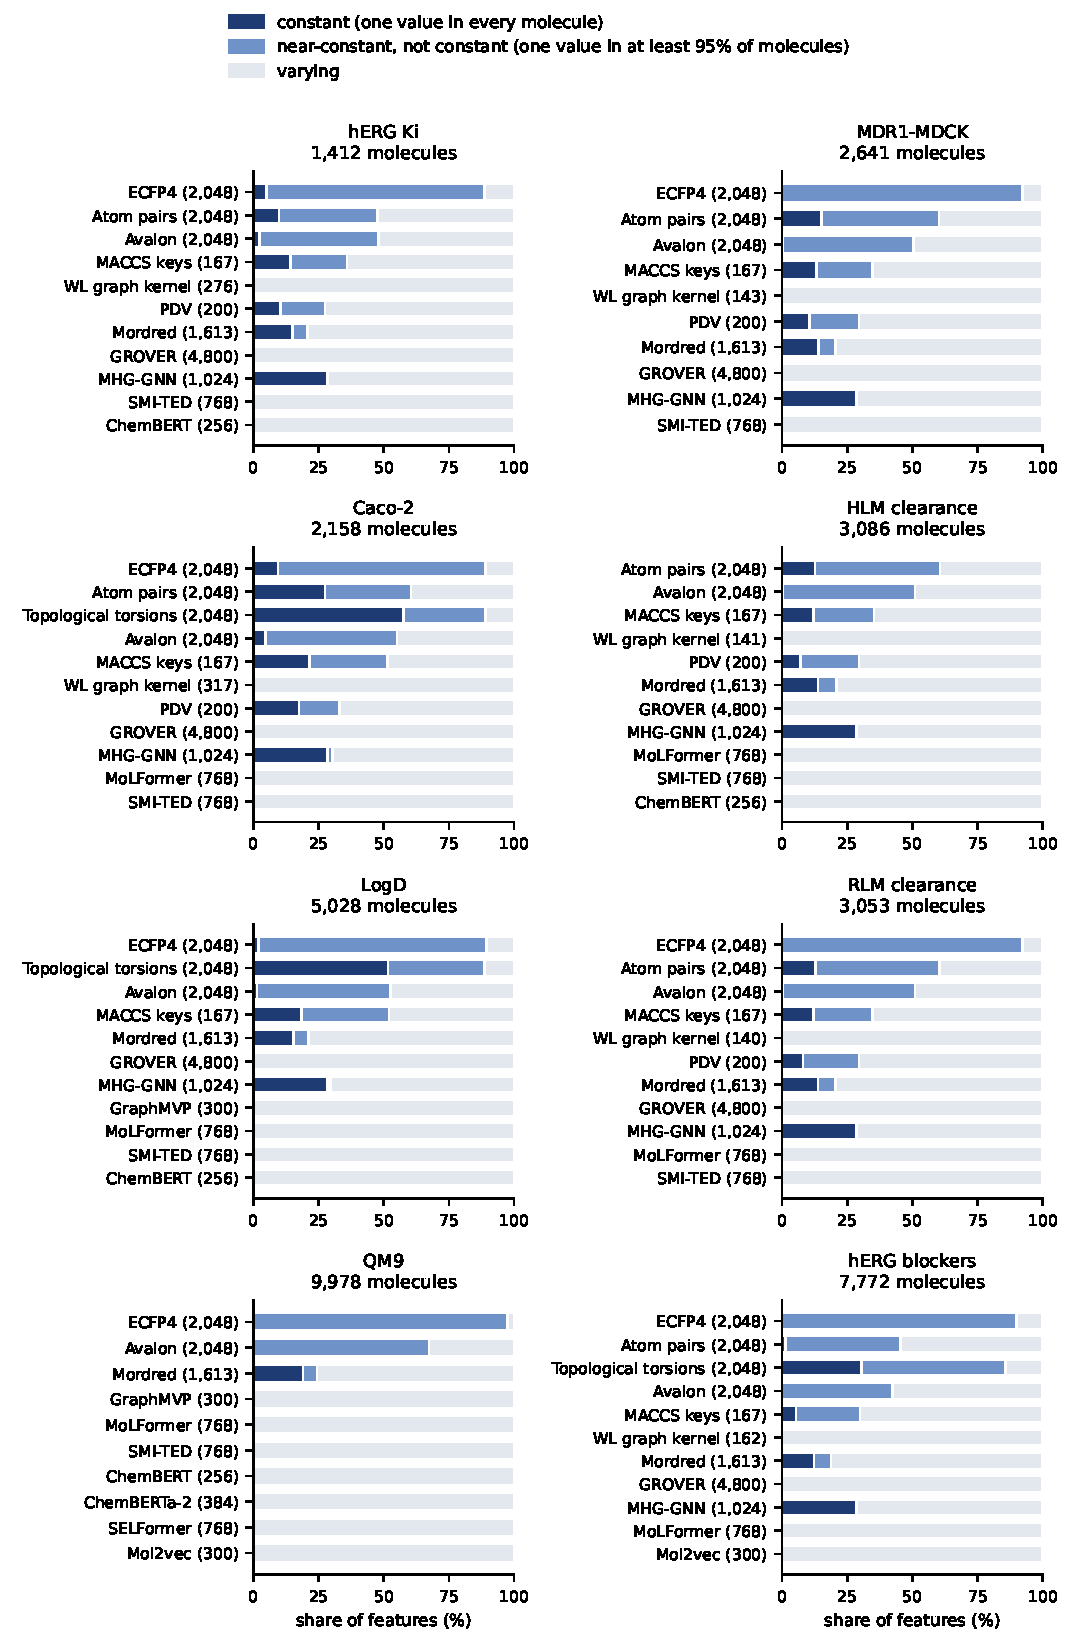
\includegraphics[width=\textwidth,height=0.72\textheight,keepaspectratio]{figures_code_input/constant_features.pdf}
\caption[Shares of constant, near-constant and varying features per representation.]{Shares of constant (dark blue), near-constant (mid blue) and varying (gray) features of each representation on eight datasets. The number of features of each representation is in parentheses.}
\label{fig:constant_features}
\end{figure}

% [TRIM3 2026-09-30] simplified
% [TRIM 2026-09-30] shortened
% TODO: review, needs manual review
Which count matters depends on the distance. Tanimoto similarity (Equation~\ref{eq:tanimoto}; the distance is $1-T$) ignores bits off in both molecules, but a bit on in every molecule raises every similarity slightly. All 105 constant ECFP4 bits on hERG $K_i$ are off. After standardization, a constant feature adds zero to a Euclidean or Manhattan distance, but a near-constant feature takes large values on the few molecules with the minority value. A bit on in 5\% of molecules becomes 4.36 on those molecules, and a bit on in one of the 1,412 hERG $K_i$ molecules becomes 37.56.

% [TRIM 2026-09-30] shortened
% [TRIM3 2026-09-30] paragraph removed

% [TRIM3 2026-09-30] paragraph removed

% [TRIM 2026-09-30] paragraph removed, text in cuts file

\todo[inline]{TODO: every cell of this table must hold a count. The dashes are representations outside that dataset's base representations; handoff in HANDOFF\_fill\_constant\_features\_tables.md.}
\begin{table}[htbp]
\centering
\small
\setlength{\tabcolsep}{4pt}
\begin{adjustbox}{max width=\textwidth,max totalheight=0.78\textheight}
\begin{tabular}{lrcccc}
\toprule
Representation & Features & hERG $K_i$ & Caco-2 & LogD & QM9 \\
 & & (1,412) & (2,158) & (5,028) & (9,978) \\
\midrule
ECFP4 & 2,048 & 105 / 1,815 & 194 / 1,826 & 39 / 1,834 & 0 / 1,997 \\
Atom pairs & 2,048 & 201 / 977 & 563 / 1,239 & -- & -- \\
Topological torsions & 2,048 & -- & 1,179 / 1,822 & 1,059 / 1,818 & -- \\
Avalon & 2,048 & 50 / 985 & 98 / 1,128 & 30 / 1,076 & 4 / 1,380 \\
MACCS keys & 167 & 24 / 60 & 36 / 86 & 31 / 87 & n/a \\
WL graph kernel & 140--317 & 0 / 0 / 276 & 0 / 0 / 317 & -- & -- \\
PDV & 200 & 21 / 55 & 35 / 66 & -- & -- \\
Mordred & 1,613 & 242 / 336 & -- & 247 / 340 & 307 / 394 \\
GROVER & 4,800 & 0 / 0 & 0 / 0 & 0 / 0 & -- \\
MHG-GNN & 1,024 & 292 / 292 & 292 / 310 & 292 / 304 & -- \\
GraphMVP & 300 & -- & -- & 0 / 0 & 0 / 0 \\
MoLFormer & 768 & -- & 0 / 0 & 0 / 0 & 0 / 0 \\
SMI-TED & 768 & 0 / 0 & 0 / 0 & 0 / 0 & 0 / 0 \\
ChemBERT & 256 & 0 / 0 & -- & 0 / 0 & 0 / 0 \\
ChemBERTa-2 & 384 & -- & -- & -- & 0 / 0 \\
SELFormer & 768 & -- & -- & -- & 0 / 0 \\
Mol2vec & 300 & -- & -- & -- & 0 / 0 \\
\bottomrule
\end{tabular}
\end{adjustbox}
\caption[Constant and near-constant features per representation, part 1.]{Constant and near-constant features of each representation on hERG $K_i$, Caco-2, LogD and QM9. Each entry gives the number of constant features and the number of near-constant features, which take one value in at least 95\% of molecules and include the constant ones. The number of molecules is under each dataset name. The width of the WL graph kernel varies, so its entries add its number of features. A dash marks a representation outside the dataset's base representations, and no MACCS keys were saved for QM9.}
\label{tab:constant_features}
\end{table}

\todo[inline]{TODO: every cell of this table must hold a count. The dashes are representations outside that dataset's base representations; handoff in HANDOFF\_fill\_constant\_features\_tables.md.}
\begin{table}[htbp]
\centering
\small
\setlength{\tabcolsep}{4pt}
\begin{adjustbox}{max width=\textwidth,max totalheight=0.78\textheight}
\begin{tabular}{lrcccc}
\toprule
Representation & Features & MDR1--MDCK & HLM clearance & RLM clearance & hERG blockers \\
 & & (2,641) & (3,086) & (3,053) & (7,772) \\
\midrule
ECFP4 & 2,048 & 1 / 1,890 & -- & 1 / 1,887 & 0 / 1,840 \\
Atom pairs & 2,048 & 308 / 1,233 & 260 / 1,240 & 262 / 1,238 & 28 / 929 \\
Topological torsions & 2,048 & -- & -- & -- & 625 / 1,754 \\
Avalon & 2,048 & 5 / 1,032 & 8 / 1,044 & 8 / 1,045 & 0 / 866 \\
MACCS keys & 167 & 22 / 58 & 20 / 59 & 20 / 58 & 9 / 50 \\
WL graph kernel & 140--317 & 0 / 0 / 143 & 0 / 0 / 141 & 0 / 0 / 140 & 0 / 0 / 162 \\
PDV & 200 & 21 / 59 & 14 / 59 & 16 / 59 & -- \\
Mordred & 1,613 & 226 / 331 & 222 / 336 & 222 / 331 & 197 / 304 \\
GROVER & 4,800 & 0 / 0 & 0 / 0 & 0 / 0 & 0 / 0 \\
MHG-GNN & 1,024 & 292 / 292 & 292 / 293 & 292 / 293 & 292 / 292 \\
MoLFormer & 768 & -- & 0 / 0 & 0 / 0 & 0 / 0 \\
SMI-TED & 768 & 0 / 0 & 0 / 0 & 0 / 0 & -- \\
ChemBERT & 256 & -- & 0 / 0 & -- & -- \\
Mol2vec & 300 & -- & -- & -- & 0 / 0 \\
\bottomrule
\end{tabular}
\end{adjustbox}
\caption[Constant and near-constant features per representation, part 2.]{Constant and near-constant features of each representation on MDR1--MDCK efflux, HLM clearance, RLM clearance and the Lhasa hERG blocker training set of 7,772 molecules. Entries read as in Table~\ref{tab:constant_features}.}
\label{tab:constant_features_b}
\end{table}

% [TRIM3 2026-09-30] simplified
RDKit's MACCS keys include an unused bit 0, hence 167 features. All constant Mordred features are zero in every molecule, except one of the 307 on QM9, which is 1. Missing or infinite descriptor values are set to 0 (Chapter~\ref{chap:method}, ``Representations by domain''), so some may be descriptors that failed to compute; we have not checked which.

% Uni-Mol v2 is left out of both tables. Its saved features are zero in every molecule on hERG Ki, LogD, MDR1-MDCK, HLM, RLM and the Lhasa hERG set (6 datasets, 768 features each). It is not in any dataset's base representations.
% The Lhasa hERG set appears once: rep_cache/herg and rep_cache/lhasa_herg hold the same 7,772 SMILES in the same order with the same labels.

% ==== END CODE INPUT ====


\subsection{Molecules with Identical Feature Vectors}
% [notes moved to thesis_notes_moved.md]

A standard fingerprint- or descriptor-based representation can produce the same feature vector for two separate molecules. In turn, models using this representation will produce a single prediction for the molecules with identical features. Identical feature vectors do not always mean that the representation has merged two different molecules, since a dataset pooled from several sources can hold two measurements of the same molecule.


% [TRIM2 2026-09-30] SMI-TED hERG Ki tie count 52 -> 56 (ties_results.json: smited tied 56, stereo_only 56)
% [CH3 CHECK 2026-09-30] "explained in Chapter 2" changed to a plain pointer: Chapter 2 names the Weisfeiler--Lehman test but does not explain it.
% TODO: Chapter 2 says ECFPs are "typically" built with chirality flags on; this paragraph says ours are built with stereochemistry off. Consider saying so explicitly, and check which setting the Chapter 3 pipeline used.
% TODO: review, needs manual review
Many fingerprints are computed without stereochemistry \citep{orsi2024map4c}. In this research, ECFP4 is built with stereochemistry off, and the 2D descriptor sets (PDV, Mordred) also ignore it, so almost every molecule they tie is a stereoisomer of another (Table~\ref{tab:flaws:ties}). Any representation read from the 2D graph merges stereoisomers, since the two share an identical graph. Separately, methods using the Weisfeiler--Lehman relabeling scheme are bounded by the 1-Weisfeiler--Lehman test (Chapter~\ref{chap:background}), so some non-isomorphic graphs also receive the same vector; the graph-kernel features tie 105 of 1,412 hERG $K_i$ molecules, 56 of which differ only in stereochemistry and 49 in more than that. Whether a learned embedding differentiates stereoisomers is up to its individual implementation. SMI-TED, a pretrained SMILES encoder, ties 56 hERG $K_i$, 633 LogD and 177 Caco-2 molecules, all stereoisomers. A tokenizer can drop stereochemistry before the model even sees the input string. The tokenizer of the ChemBERTa-77M-MTR checkpoint (ChemBERTa-2 in Table~\ref{tab:constant_features}, called ChemBERTa in Chapter~\ref{chap:robustness}) gives 72 of the 1,415 hERG $K_i$ molecules of Chapter~\ref{chap:robustness} the same token sequence as another molecule. If stereoisomers did not differ in activity, this would not matter. However, stereoisomers can differ in measured activity \citep{Nguyen2006}, meaning these representations are all lacking potentially important chemical information.

% [TRIM3 2026-09-30] simplified
% CODE TODO [handled, see CODE INPUT blocks below]: paragraphs 4/5/6 + table + figure. Basically finish it out
% ==== CODE INPUT: new, needs review ====
% Numbers: scratchpad/thesis_code_todo/ties/ties_results.json (script ties/ties.py; table rows ties/table.py; figure ties/figure.py, pair in ties/figure_pair.json).
% Paragraph 4: the measurement.
For each dataset and representation, we grouped molecules with identical stored feature vectors. A tied molecule is a repeat if another molecule in its group has the same InChIKey, a featurization failure if its vector is all zeros, and a distinct molecule otherwise. A distinct molecule is stereo-only when every molecule sharing its vector has the same InChIKey connectivity block, so they differ only in stereochemistry.

% [TRIM3 2026-09-30] simplified
Every molecule in a tied group receives the same prediction, and the prediction with the lowest squared error is the group's mean label. The lowest error any model can reach is therefore
\begin{equation}
\mathrm{RMSE}_{\min} = \sqrt{\frac{1}{n}\sum_{G}\sum_{i \in G}\left(y_i - \bar{y}_G\right)^2},
\end{equation}
where $n$ is the number of molecules, $G$ runs over the tied groups and $\bar{y}_G$ is the mean label of group $G$. The best $R^2$ is $1 - \mathrm{RMSE}_{\min}^2 / \mathrm{Var}(y)$. The label spread of a tied group is its highest label minus its lowest. Repeat p$K_i$ measurements of one compound disagree by about $0.54$ log units \citep{Kramer2012}, so a larger p$K_i$ spread is not explained by measurement noise alone. We counted ties on hERG $K_i$ (deduplicated by InChIKey), LogD and Caco-2, for each dataset's base representations and augmentation features (small feature sets added to the hybrid after it is built, Chapter~\ref{chap:method}, ``Augmentation'').

% [TRIM3 2026-09-30] simplified
% [TRIM 2026-09-30] shortened
% Paragraph 5: what was found.
No tie came from a repeated molecule or a row of zeros, so every tie is a merge made by the representation (Table~\ref{tab:flaws:ties}). Atom pairs, PDV, Mordred and SMI-TED tie only stereoisomers. ECFP4, Avalon and topological torsions tie mostly stereoisomers, plus a few molecules that are not stereo-only. On hERG $K_i$, ECFP4, atom pairs, PDV, Mordred and SMI-TED all tie the same 56 molecules in the same 26 groups, so concatenating any of these five leaves all 56 tied. The WL graph kernel ties 49 hERG $K_i$ and 26 Caco-2 molecules that are not stereo-only. The MACCS keys tie the most molecules on every dataset, mostly not stereo-only (only 30 of 377 are stereo-only on hERG $K_i$). The 3D augmentation representations (3D pharmacophore, USR, USRCAT and Coulomb matrix) and the learned embeddings ChemBERT, GROVER, MHG-GNN, MoLFormer and GraphMVP tie none. % CHECK: the ChemBERT count comes from the cached chembert.npy (256 features). Whether that cache matches the current featurizer code is unverified.
Concatenating all of a dataset's representations leaves no molecule tied on any of the three datasets.

% [TRIM3 2026-09-30] simplified
On hERG $K_i$ the lowest reachable error is at most $0.134$ p$K_i$ (MACCS keys), small against a label standard deviation of $0.915$ p$K_i$. One tied group can still spread widely: the largest ECFP4 spread on hERG $K_i$ is $1.14$ p$K_i$, more than twice the repeat-measurement scale (Figure~\ref{fig:flaws:stereo_pair}). The best any ECFP4 model can predict for this pair is their mean, $5.59$ p$K_i$, which leaves each molecule $0.57$ p$K_i$ from its measured value.

% [TRIM3 2026-09-30] simplified
On hERG $K_i$, the mean label spread of a tied group is $0.28$ p$K_i$ under ECFP4 and $0.39$ p$K_i$ under the MACCS keys. Of the 26 ECFP4 groups, 24 hold different labels and 6 differ by more than $0.54$ p$K_i$. Of the 153 MACCS groups, 138 hold different labels and 38 differ by more than $0.54$ p$K_i$.

\begin{figure}[!htbp]
\centering
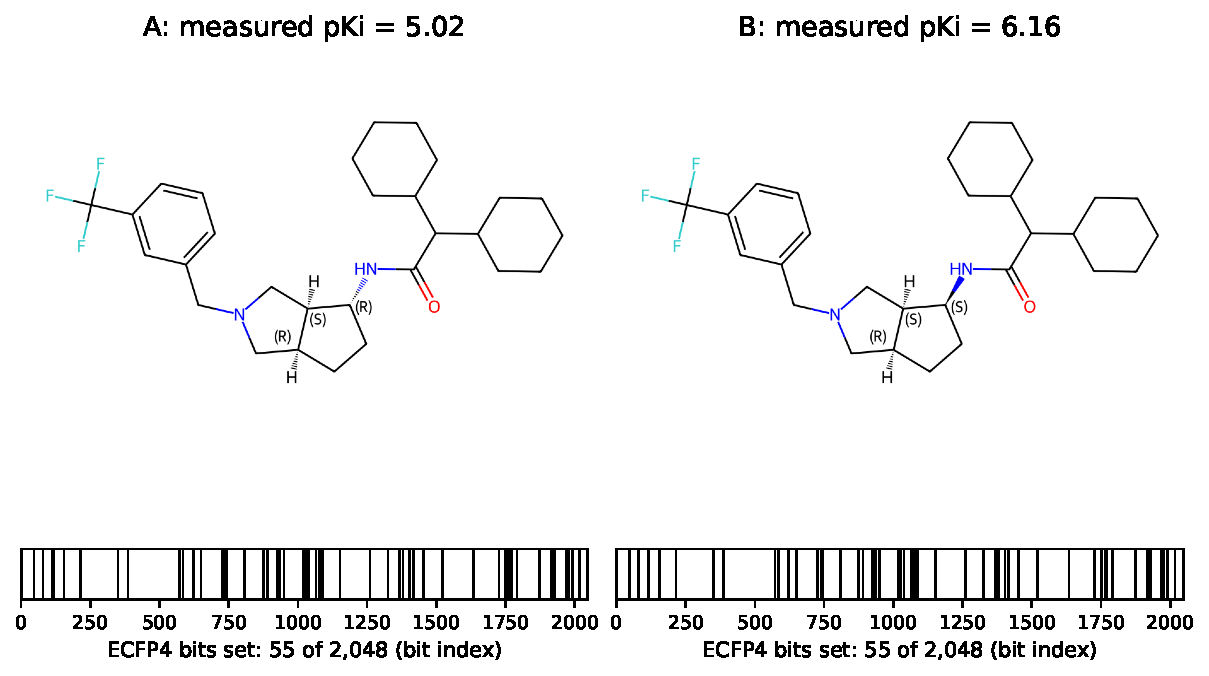
\includegraphics[width=\textwidth,height=0.72\textheight,keepaspectratio]{figures_code_input/herg_ki_ecfp4_stereo_pair.pdf}
\caption[Two hERG $K_i$ stereoisomers with identical ECFP4 vectors.]{Two hERG $K_i$ stereoisomers with identical ECFP4 vectors, which differ at the carbon bearing the amide nitrogen (R in A, S in B). The top row shows the structures with their measured p$K_i$ values, and the bottom row shows the 55 of 2,048 ECFP4 bits set in both.}
\label{fig:flaws:stereo_pair}
\end{figure}

% [TRIM3 2026-09-30] simplified
% Paragraph 6: consequence for activity cliffs and for neighbor-based methods.
The structure--activity landscape index of a pair of molecules $i$ and $j$ is
\begin{equation}
\mathrm{SALI}_{ij} = \frac{|y_i - y_j|}{1 - \mathrm{sim}(i,j)}
\end{equation}
\citep{Guha2008}. A tied pair has similarity 1, so its index is infinite whenever the labels differ. Such a tie is the most extreme activity cliff possible, and an artifact of the representation. A nearest-neighbor method sees a tied neighbor at distance 0 with a different label. % CHECK: sec:flaws:neighbors is not yet a label in thesis.tex; it comes from another CODE INPUT fragment.
It may then flag a correct label as noise (Section~\ref{sec:flaws:neighbors}).

% Table: one row per dataset x representation that ties any molecule.
\begin{table}[htbp]
\centering
\small
\setlength{\tabcolsep}{4pt}
\begin{adjustbox}{max width=\textwidth,max totalheight=0.78\textheight}
\begin{tabular}{llrrrrrr}
\toprule
Dataset & Representation & Molecules & Tied & Stereo- & Best & Best & Largest \\
 & & & & only & RMSE & $R^2$ & spread \\
\midrule
hERG $K_i$ (p$K_i$) & ECFP4 & 1,412 & 56 (4.0\%) & 56 & 0.041 & 0.998 & 1.14 \\
 & Atom pairs & 1,412 & 56 (4.0\%) & 56 & 0.041 & 0.998 & 1.14 \\
 & PDV & 1,412 & 56 (4.0\%) & 56 & 0.041 & 0.998 & 1.14 \\
 & Mordred & 1,412 & 56 (4.0\%) & 56 & 0.041 & 0.998 & 1.14 \\
 & SMI-TED & 1,412 & 56 (4.0\%) & 56 & 0.041 & 0.998 & 1.14 \\
 & Avalon & 1,412 & 66 (4.7\%) & 56 & 0.049 & 0.997 & 1.20 \\
 & WL graph kernel & 1,412 & 105 (7.4\%) & 56 & 0.071 & 0.994 & 1.49 \\
 & MACCS keys (aug.) & 1,412 & 377 (26.7\%) & 30 & 0.134 & 0.978 & 1.80 \\
\midrule
LogD (log units) & ECFP4 & 5,028 & 641 (12.7\%) & 633 & 0.044 & 0.999 & 1.00 \\
 & Mordred & 5,028 & 633 (12.6\%) & 633 & 0.043 & 0.999 & 1.00 \\
 & SMI-TED & 5,028 & 633 (12.6\%) & 633 & 0.043 & 0.999 & 1.00 \\
 & Avalon & 5,028 & 647 (12.9\%) & 629 & 0.047 & 0.998 & 1.40 \\
 & Topological torsions & 5,028 & 675 (13.4\%) & 631 & 0.047 & 0.998 & 1.10 \\
 & MACCS keys (aug.) & 5,028 & 2,343 (46.6\%) & 437 & 0.220 & 0.965 & 2.80 \\
\midrule
Caco-2 (log units) & ECFP4 & 2,158 & 179 (8.3\%) & 177 & 0.027 & 0.996 & 0.74 \\
 & Atom pairs & 2,158 & 177 (8.2\%) & 177 & 0.027 & 0.996 & 0.74 \\
 & PDV & 2,158 & 177 (8.2\%) & 177 & 0.027 & 0.996 & 0.74 \\
 & SMI-TED & 2,158 & 177 (8.2\%) & 177 & 0.027 & 0.996 & 0.74 \\
 & Avalon & 2,158 & 181 (8.4\%) & 177 & 0.027 & 0.996 & 0.74 \\
 & Topological torsions & 2,158 & 186 (8.6\%) & 177 & 0.029 & 0.996 & 0.74 \\
 & WL graph kernel & 2,158 & 203 (9.4\%) & 177 & 0.028 & 0.996 & 0.74 \\
 & MACCS keys (aug.) & 2,158 & 804 (37.3\%) & 139 & 0.111 & 0.935 & 1.72 \\
\bottomrule
\end{tabular}
\end{adjustbox}
\caption[Molecules that share a feature vector with another molecule.]{Molecules that share their feature vector with at least one other molecule, for each representation that ties at least two molecules. Tied gives the number and share of such molecules, and Stereo-only counts those tied only with their own stereoisomers. Best RMSE and best $R^2$ are reached by predicting the mean label of each tied group, the lowest error any model can reach. Largest spread is the largest label range within one tied group, in the dataset's label units, and (aug.) marks an augmentation representation.}
\label{tab:flaws:ties}
\end{table}

% ==== END CODE INPUT ====




\section{Flaws in Similarity and Other Pairwise Computations}\label{sec:flaws:similarity} % CODE INPUT: label added, needs review
% [notes moved to thesis_notes_moved.md]

% TODO: review, needs manual review
Section~\ref{sec:flaws:representations} described flaws of individual representations. Here we ask what happens when two molecules are compared through one of them. These pairwise comparisons (Chapter~\ref{chap:background}) can violate the similarity assumption, and we discuss both the representation and the coefficient.


The standard way of comparing two small molecules is the Tanimoto coefficient on ECFPs \citep{LopezPerez2024}, although the coefficient applies to any bit vector. Independently, the Tanimoto coefficient is described as the ``coefficient of choice'' for molecular similarity \citep{Bajusz2015}, while the Morgan fingerprint, ECFP4 in this research, ranks among the strongest fingerprints for virtual screening and target prediction \citep{Capecchi2020}. ECFP4 and ECFP6 specifically, alongside topological torsion, rank among the best of 28 fingerprints tested for ordering diverse structures by similarity \citep{OBoyle2016}. However, it is not a one-size-fits-all solution. Across 96,456 human metabolites, 72.9\% had an ECFP4 nearest neighbor at Tanimoto distance 0 \citep{Capecchi2020}, again running into the issue of the representation lacking stereochemical information and more generally being unable to distinguish molecules. 

% [TRIM3 2026-09-30] simplified
% [TRIM 2026-09-30] shortened
% CODE INPUT: references filled in (Equation~\ref{eq:tanimoto_kernel}; the labels sec:flaws:representations, sec:flaws:similarity, sec:flaws:consequences, sec:flaws:constant, sec:flaws:neighbors, sec:lnl_background were added at their headings). Needs review.


All a similarity coefficient can do is compare every feature, yet it cannot tell which features matter to the prediction task at hand. And the similarity assumption holds only relative to such a measure, which is fixed by the choice of representation. To estimate what this costs, we categorize a representation's features into those relevant to the task, $R$, and those that are irrelevant, $I$. We take the squared Euclidean distance as a sum over both:
\begin{equation}
d^2(\mathbf{x},\mathbf{y}) = \sum_{j \in R}(x_j-y_j)^2 + \sum_{j \in I}(x_j-y_j)^2 .
\label{eq:distance_split}
\end{equation}

Every irrelevant feature that varies adds one further term, so the irrelevant part grows linearly with $|I|$. After standardization each feature contributes the same amount on average over all pairs, so the share of the distance carrying signal is about $|R|/(|R|+|I|)$. When we use a general-purpose representation like ECFP4 on a dataset spanning a small portion of the chemical space, $|I|$ can be a lot larger than $|R|$. Features that remain constant across the dataset contribute nothing. Rather, the damage comes from features that vary but bear no relation to the property in question. The worst case scenario involves a single rare bit set in only a handful of molecules. After standardization, uncommon bits take on larger values, outweighing common features that may be more relevant. This is why the near-constant count in Section~\ref{sec:flaws:constant} matters more than the constant count.


Larger representations, or higher dimensionality, compound the problem. As the number of dimensions grows, the nearest and farthest molecules end up at nearly the same distance, meaning that these pairwise distances are less able to discriminate, as explained in Chapter~\ref{chap:background}. Two measures of this effect are the relative contrast, defined as the difference between the largest and smallest measured distance divided by the smallest, and hubness, a measure of how unevenly the molecules appear in other molecules' nearest neighbors \citep{Radovanovic2010}; we do not compute them here. These errors propagate along larger data pipelines, starting from the representation into similarity, from similarity into the set of neighbors a molecule is compared against, and from there into a prediction of some kind. 

% CODE TODO [handled, see CODE INPUT blocks below]: paragraphs 6 + 7 + figure + table, finish this out


% [TRIM3 2026-09-30] simplified
% ==== CODE INPUT: new, needs review ====
% Numbers: /Users/apunt/repos/KIRBy/scratchpad/thesis_code_todo/distance/results_all.json
% Scripts: compute.py, overlap.py, mcs.py, figure.py, collect.py in the same folder.
% Paragraph 5 result (cliff counts) is the first paragraph below; it can move up to Paragraph 5.
% HLM clearance (adme_hlm) is not in Table~\ref{tab:datasets}; drop its rows if it is not a thesis dataset.
% The cliff rule cited to Chapter 2 is so far only in that section's NOTES ("This thesis counts cliffs with a different rule"); its prose must state it.
% [TRIM 2026-09-30] shortened
% [CH3 CHECK 2026-09-30] The rebuilt Chapter 2 does not state a 0.55 rule; it gives the MoleculeACE rule (similarity above 90% under one of three measures, a tenfold difference in K_i or EC50). The opening sentence now says this chapter uses its own rule. Needs your check that this is the intended framing.
% TODO: review, needs manual review
Chapter~\ref{chap:background} defines an activity cliff and gives the MoleculeACE rule, which uses three similarity measures and a tenfold difference in potency. Here we count cliffs with a simpler rule on one measure. A pair is similar at an ECFP4 Tanimoto similarity of at least 0.55, and the activity gap is set per dataset so that 15\% of molecules are cliffs (14.5\% on LogD, as the share moves in steps). The gap therefore varies between datasets (Table~\ref{tab:flaws:distance_summary}). On hERG $K_i$ it is 1.76 p$K_i$, with 211 of the 1,412 molecules cliffs. On QM9, only 1,093 pairs among 9,978 molecules reach 0.55, and the gap is 0.05~eV, or 0.06 times the median absolute deviation of the labels. On the three datasets from the Biogen set (RLM clearance, MDR1--MDCK efflux and HLM clearance) it is 0.20 to 0.34 log units, or 0.50 to 0.60 times the median absolute deviation.

% [TRIM3 2026-09-30] simplified
The count also depends on the representation. Keeping each dataset's gap, we replaced ECFP4 with each other base representation, taking as similar as many of that representation's closest pairs as ECFP4 calls similar. On hERG $K_i$ the number of cliff molecules then ranges from 138 (atom pairs) to 267 (WL graph kernel). Only 57\% to 74\% of the pairs that ECFP4 calls similar are among another representation's closest pairs, and on QM9 1\% to 24\% (Additional file~\ref{app:add:flaws}).

% [TRIM3 2026-09-30] simplified
% [TRIM 2026-09-30] shortened
We ask two questions of a distance. First, across all pairs, does distance track the difference in property? We summarize the neighborhood-behavior plot of \citet{Patterson1996}, descriptor distance against activity difference for every pair, as the Spearman correlation between pair distance and absolute label difference. Second, can each molecule's label be predicted as the mean label of its five nearest neighbors?

% [TRIM3 2026-09-30] simplified
% [TRIM 2026-09-30] shortened
We computed both for every base representation of seven regression datasets: the six small-molecule regression datasets of Table~\ref{tab:dataset_reps} (Chapter~\ref{chap:method}) and HLM clearance, a third Biogen dataset not used elsewhere in this thesis. Binary representations were compared by Tanimoto distance, and all others by Manhattan distance (next subsection) on standardized, non-constant features. For the all-pairs correlation, datasets above 2,000 molecules were reduced to a random sample of 2,000. For the neighbor prediction, each molecule's five neighbors were drawn from other scaffold groups.

% [TRIM3 2026-09-30] simplified
% [RESTORE 2026-09-30] Ch4-7
Across the 70 combinations of dataset and representation, the all-pairs correlation ranged from $-0.04$ to 0.23 and was below 0.10 in 44 of the 70. The Spearman correlation of the five-neighbor prediction ranged from 0.29 to 0.89, and it was the larger of the two in all 70 (Table~\ref{tab:flaws:distance_summary}). On hERG $K_i$, ECFP4 gives an all-pairs correlation of 0.06, while its five-neighbor prediction reaches 0.72, with an RMSE of 0.63 p$K_i$ against a label standard deviation of 0.92 p$K_i$.

% [TRIM3 2026-09-30] simplified
Figure~\ref{fig:flaws:herg_pairs} shows why the two differ on hERG $K_i$. Of the 996,166 pairs, 93\% have an ECFP4 Tanimoto similarity below 0.20 and 1.1\% reach 0.55. The median label difference is 0.81 p$K_i$ over all pairs but 0.20 to 0.30 p$K_i$ above a similarity of about 0.4, though 8.3\% of the 774 pairs at 0.8 or above differ by more than 1 p$K_i$. Under Mordred, the closest 5\% of pairs have a median difference of 0.44 p$K_i$, and every other 5\% a median of 0.78 to 1.11 p$K_i$. The signal sits in this thin tail of close pairs. The all-pairs correlation is set mostly by the other 95\%, whereas a five-neighbor prediction looks only at each molecule's closest pairs.

% [TRIM3 2026-09-30] simplified
A third view asks how often two representations agree on each molecule's five nearest neighbors. We compared ECFP4, SMI-TED and Mordred (PDV on Caco-2, where Mordred is not a base representation). HLM clearance, which lacks ECFP4 among its base representations, used its stored ECFP4 features. On hERG $K_i$ any two of the three share on average 0.47 to 0.52 of each molecule's five neighbors, and on the three Biogen datasets and QM9 only 0.13 to 0.21 (Table~\ref{tab:flaws:neighbor_overlap}).

% [TRIM3 2026-09-30] simplified
A fourth view asks whether fingerprint distance agrees with a structural distance. For 500 random pairs per dataset we computed the maximum common substructure (MCS) with RDKit \citep{rdkit}, allowing each pair 2 seconds. The MCS distance is $1 - n/(a+b-n)$, where $n$ is the number of atoms in the common substructure and $a$ and $b$ are the numbers of heavy atoms of the two molecules. Its Spearman correlation with ECFP4 Tanimoto distance ranged from 0.20 (hERG $K_i$ and HLM clearance) to 0.51 (Caco-2 and LogD).

% [TRIM3 2026-09-30] simplified
% [RESTORE 2026-09-30] Ch4-9
% TODO: review, needs manual review -- related-work sentences moved to the end of the Introduction's related-work paragraph
Every method in Section~\ref{sec:flaws:consequences} takes a similarity as input and inherits the dilution described here.

\begin{figure}[!htbp]
\centering
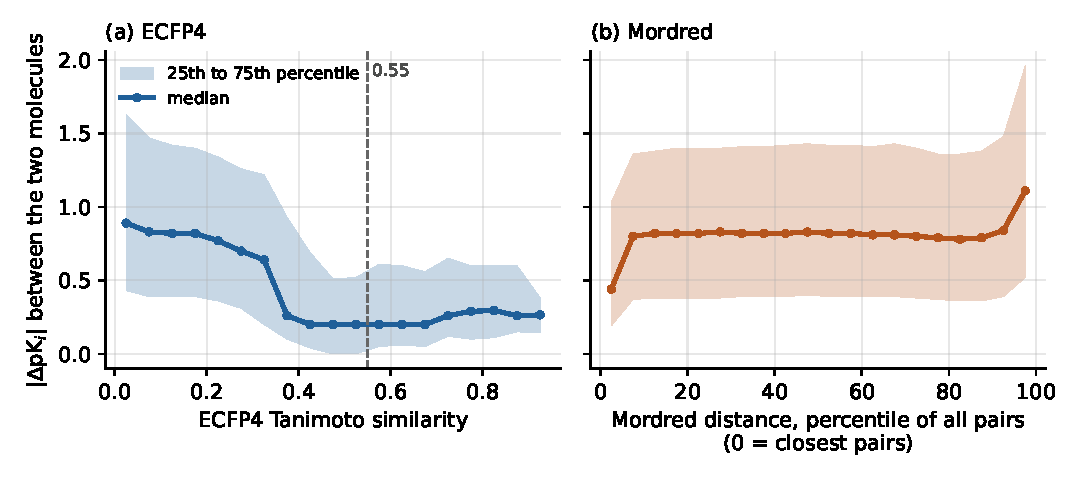
\includegraphics[width=\textwidth,height=0.72\textheight,keepaspectratio]{figures_code_input/herg_ki_pair_distance_vs_dpki.pdf}
\caption[Absolute p$K_i$ difference against pair distance on hERG $K_i$.]{Absolute p$K_i$ difference against distance for all 996,166 pairs of the 1,412 hERG $K_i$ molecules, with the median in each bin (markers) and the interquartile range (shaded). a) ECFP4 Tanimoto similarity in bins of 0.05, omitting bins with fewer than 20 pairs, with the activity-cliff threshold of 0.55 dashed. b) Manhattan distance on standardized Mordred features, as a percentile of all pairs.}
\label{fig:flaws:herg_pairs}
\end{figure}


\begin{table}[t]
\centering
\small
\setlength{\tabcolsep}{3.5pt}
\begin{adjustbox}{max width=\textwidth,max totalheight=0.78\textheight}
\begin{tabular}{lrrrrrrrrl}
\toprule
 & & \multicolumn{3}{c}{All pairs} & \multicolumn{3}{c}{Five neighbors} & \multicolumn{2}{c}{Cliffs} \\
\cmidrule(lr){3-5}\cmidrule(lr){6-8}\cmidrule(lr){9-10}
Dataset & Molecules & ECFP4 & Desc. & SMI-TED & ECFP4 & Desc. & SMI-TED & Molecules & Gap \\
\midrule
hERG $K_i$ & 1,412 & 0.06 & 0.07 & 0.09 & 0.72 & 0.72 & 0.69 & 211 & 1.76 p$K_i$ \\
LogD & 5,028 & 0.12 & 0.06 & 0.10 & 0.76 & 0.80 & 0.76 & 731 & 2.90 log \\
Caco-2 & 2,158 & 0.08 & 0.18 & 0.14 & 0.59 & 0.62 & 0.57 & 324 & 1.21 log \\
RLM clearance & 3,053 & 0.02 & 0.07 & 0.04 & 0.36 & 0.49 & 0.46 & 458 & 0.34 log \\
MDR1--MDCK efflux & 2,641 & 0.02 & 0.16 & 0.10 & 0.51 & 0.58 & 0.59 & 397 & 0.20 log \\
HLM clearance & 3,086 & $-0.00$\textsuperscript{\textdagger} & 0.07 & 0.03 & 0.37\textsuperscript{\textdagger} & 0.49 & 0.45 & 462 & 0.27 log \\
QM9 & 9,978 & 0.19 & 0.18 & 0.13 & 0.88 & 0.84 & 0.85 & 1,495 & 0.05 eV \\
\bottomrule
\end{tabular}
\end{adjustbox}
\caption[All-pairs correlation, five-nearest-neighbor prediction and activity cliffs per dataset.]{All-pairs correlation, five-nearest-neighbor prediction and activity cliffs for each dataset. All pairs gives the Spearman correlation between pair distance and absolute label difference, on a sample of 2,000 molecules for larger datasets. Five neighbors gives the Spearman correlation between each label and the mean label of its five nearest neighbors from other scaffold groups. Desc.\ is Mordred, or PDV on Caco-2. Cliffs gives the number of cliff molecules and the label gap, where a cliff pair has an ECFP4 Tanimoto similarity of at least 0.55 and a label difference above the gap, which is set so that 15\% of molecules are cliffs. \textsuperscript{\textdagger}ECFP4 is not a base representation of this dataset. Additional file~\ref{app:add:flaws} gives every representation.}
\label{tab:flaws:distance_summary}
\end{table}


\begin{table}[t]
\centering
\small
\setlength{\tabcolsep}{4pt}
\begin{adjustbox}{max width=\textwidth,max totalheight=0.78\textheight}
\begin{tabular}{llrrrrrr}
\toprule
 & & \multicolumn{3}{c}{Five-neighbor overlap} & \multicolumn{3}{c}{ECFP4 against MCS} \\
\cmidrule(lr){3-5}\cmidrule(lr){6-8}
Dataset & Desc. & \makecell{ECFP4--\\Desc.} & \makecell{ECFP4--\\SMI-TED} & \makecell{Desc.--\\SMI-TED} & Spearman & Pairs & \makecell{Timed\\out} \\
\midrule
hERG $K_i$ & Mordred & 0.52 & 0.50 & 0.47 & 0.20 & 495 & 5 \\
LogD & Mordred & 0.38 & 0.41 & 0.41 & 0.51 & 494 & 6 \\
Caco-2 & PDV & 0.38 & 0.41 & 0.38 & 0.51 & 492 & 8 \\
RLM clearance & Mordred & 0.15 & 0.21 & 0.18 & 0.28 & 500 & 0 \\
MDR1--MDCK efflux & Mordred & 0.15 & 0.20 & 0.17 & 0.26 & 500 & 0 \\
HLM clearance & Mordred & 0.15 & 0.21 & 0.18 & 0.20 & 500 & 0 \\
QM9 & Mordred & 0.13 & 0.18 & 0.21 & 0.46 & 500 & 0 \\
\bottomrule
\end{tabular}
\end{adjustbox}
\caption[Agreement between representations per dataset.]{Agreement between representations for each dataset. Five-neighbor overlap is the mean fraction of a molecule's five nearest neighbors, drawn from other scaffold groups, that two representations share. ECFP4 against MCS gives the Spearman correlation between ECFP4 Tanimoto distance and MCS distance on 500 random pairs, with the numbers of pairs used and left out at the 2-second limit.}
\label{tab:flaws:neighbor_overlap}
\end{table}
% ==== END CODE INPUT ====


\subsection{Distance Metrics for Continuous Molecular Descriptors}
% [notes moved to thesis_notes_moved.md]

% [TRIM2 2026-09-30] list cut to the metrics Chapters 5 and 6 use; false pointer to sec:flaws:neighbors dropped
% TODO: review, needs manual review
Binary fingerprints are compared with the Tanimoto coefficient (Chapter~\ref{chap:background}), but continuous features need a distance. The exploratory study of Section~\ref{sec:lnl_motivation} used the following four:

% [TRIM2 2026-09-30] Chebyshev, correlation, Canberra and Bray--Curtis removed
\begin{itemize}
    \item Euclidean ($L_2$): standard geometric distance, $d(x, y) = \sqrt{\sum_i (x_i - y_i)^2}$
    \item Manhattan ($L_1$): sum of absolute differences, $d(x, y) = \sum_i |x_i - y_i|$, more robust to outlier features
    \item Cosine: angle-based, $d(x, y) = 1 - \frac{x \cdot y}{\|x\| \|y\|}$, invariant to magnitude
    \item Mahalanobis: covariance-adjusted distance, $d(x,y)=\sqrt{(x-y)^\top S^{-1}(x-y)}$, where $S$ is the feature covariance estimated on the training molecules \citep{Mahalanobis1936}
\end{itemize}

% [TRIM2 2026-09-30] Bray--Curtis/Canberra sentence removed
All features are standardized to zero mean and unit variance before distances are computed, so that features on different scales contribute equally. % TODO: REVIEW MODIFICATION -- formula checked against the code on 2026-09-29: tests/noise_mitigation_advanced.py:208-219 shifts Bray--Curtis only; Canberra only adds 1e-10. The Mahalanobis covariance matrix is singular here, as the features outnumber the molecules, so its pseudo-inverse is used.

% [TRIM3 2026-09-30] simplified
% [TRIM2 2026-09-30] "four of these" became "four distances": after the list cut, Minkowski is not in the list and Mahalanobis is
% TODO: review, needs manual review
Chapters~\ref{chap:method} and~\ref{chap:similarity} use four distances: Manhattan by default, Euclidean, cosine, and Minkowski with $p=0.5$, $d(x,y)=\left(\sum_i |x_i-y_i|^{0.5}\right)^{2}$, a dissimilarity rather than a metric because it breaks the triangle inequality. Feature weights from the hybrid are applied after standardization (Chapter~\ref{chap:similarity}).


% CODE INPUT: heading added. The notes block below had no \section, but the chapter introduction refers to it as Section~\ref{sec:flaws:consequences}. Needs review.
\section{Consequences for Similarity-Based Methods}\label{sec:flaws:consequences}
% [notes moved to thesis_notes_moved.md]


% [TRIM2 2026-09-30] last sentence ("When I was exploring LNL methods...") deleted
We have identified flaws in the representations themselves and in the similarities computed over them. For a given molecule, its set of neighbors, built from one representation and one distance, is the input to several other processes such as predicting a molecule's activity from its nearest neighbors, detecting noisy labels by comparing a label against its neighbors' labels, defining an applicability domain by distance to the training set \citep{Tropsha2010}, grouping molecules into clusters for data splits \citep{Butina1999}, identifying activity cliffs, and, in federated learning, weighting each site's vote on a molecule by that molecule's distance to the site's own data \citep{Hanser2025}. If the distance is flawed, then every application of distance will suffer the consequences.

Section~\ref{sec:lnl_motivation} reports the exploratory LNL study, in which the 20 configurations with the lowest retention under noise all used a distance. Section~\ref{sec:flaws:neighbors} turns to noise detection by neighbors, the most direct use of similarity in this thesis. 

% CODE TODO [handled, see CODE INPUT blocks below]: so I won't be just reporting my confirmation report. The reviewers won't see that. that material needs to be transferred over, and ideally shortened. this will take a lot... And I have enough there that you can go ahead and copy the langauge (maybe remove some) but refrain from adding your own flair unless it's absoltuely necessary. I've been ignoring every other instruction of yours to cite the confirmation report but now it's unavoidable. This needs fixing. And the output shouldn't be bullets it should just be a smaller version of what I wrote before with results. This should affect this section and the next.
\subsection{Exploratory Study of Learning with Noisy Labels}\label{sec:lnl_motivation}
% [notes moved to thesis_notes_moved.md]

% [OLD TEXT replaced by CODE INPUT below]
% Numerous studies have explored Learning with Noisy Labels (LNL) in the broader context of ML, as well as specifically for QSAR models. \citet{Song2022} provide a comprehensive review of Deep LNL, identifying five main approaches: (i) modifying architectures to better handle noise in training; (ii) employing regularization to reduce overfitting to noise; (iii) adjusting loss functions to be less sensitive to outliers or label flips; (iv) post-processing to adjust the weights for noisy data; and (v) sample selection to select presumably clean data to pre-train. \citet{Cortes2015} examined 12 different algorithms across 12 datasets and 10 noise levels, finding that no single algorithm was overall best at maintaining predictive performance in the presence of noise; certain algorithms perform better or worse at different levels of noise. This is a recurring theme in LNL research: there is no universal solution to handling noise with experimental endpoints.
% % TODO make this flow
% There are a wide variety of approaches to LNL, spanning sample selection, meta-learning, curriculum learning, and iterative refinement \citep{Song2022}. Cheminformatics data presents additional challenges in the form of high-dimensional molecular representations and dealing with a wide variety of chemical domains with various similarities and relationships. In this chapter, we explore a set of 12 LNL methods in the context of QSAR modeling. We examine the impact of uncertainty quantification, molecular distance metrics, and alternative loss functions in the hopes of improving performance under label noise. We tested 221 total configurations across LNL methods, loss functions, distance metrics, and molecular representations. Notably, we found that molecular representation choice explains even less variance under LNL methods. We also identified the following LNL techniques which showed promise on the tasks at hand: heteroscedastic GP, curriculum learning, and sample selection methods. The work was meant to connect the representation and uncertainty quantification insights found in Chapter~\ref{chap:robustness} with more classical noise mitigation techniques as a means of determining broader research directions. 
%
% One of the most prominent outcomes was that distance-augmented methods performed significantly worse than ones that did not incorporate any sense of distance or molecular similarity. An ANOVA test was run on the different adapted factors and shows that distance metric usage is the dominant factor in variance in $R^2$.. When ranking the performance of methods, all 20 worst-performing configurations with respect to noise robustness used distance metrics, not a single one achieved both high baseline ($R^2 > 0.6$) and high noise retention ($> 80\%$). This pattern was observed across standard distance types (Euclidean, Manhattan, Cosine, Mahalanobis) and a chemistry-aware metric (Tanimoto coefficient). 
%
% Building upon the exploratory study above, we decided to investigate alternative featurization techniques. There are multiple possible explanations behind the poor performance of distance metrics, first being that a singular molecular representation lacks sufficient information for distance calculations, with and possibly even without noise. These representations all encode different types of molecular information, PDVs encode global molecular properties, ECFPs contain substructure information, and MPNNs such as MHG-GNNs capture 3D structural features. These single sources of data may not be sufficient for robust similarity estimation. Additionally, some of these representations are sparse and contain a large number of features that are not relevant to molecules of a given domain. 
%
% The main issue we identified here is that when a large proportion of dimensions are uninformative, similarity measures become dominated by those uninformative features, causing exponential growth in the number of irrelevant pairwise interactions as dimensionality increases. This is what we sought to address by developing a representation with informative features and low dimensionality. We do so by creating a budget-constrained hybrid representation, which takes high-importance features from a variety of sources. These hybrid representations concatenate the top-ranked features by importance from a selection of base representations. 
% ==== CODE INPUT: new, needs review ====
% Transferred from the confirmation report (paper.tex, Chapter 4 "Exploring techniques for learning with noisy labels for QSAR", and the opening of Chapter 5), shortened, with the "Change:" bullets applied.
% [TRIM3 2026-09-30] simplified
% TODO: Ch3 update -- re-check the Chapter 3 results quoted in this paragraph against the updated chapter.
% [CH3 CHECK 2026-09-30] re-checked against the rebuilt Chapter 3 Conclusions: model family is the dominant factor for robustness (AUC_norm); representation explains at most 11.2% of its variance.
% [TRIM2 2026-09-30] clean-performance half of the Chapter 3 sentence cut
% TODO: review, needs manual review
This section reuses an exploratory study of LNL carried out earlier in this project. In Chapter~\ref{chap:robustness}, model family explained the largest share of the variance in robustness to label noise, and representation at most 11.2\%, so we asked whether training methods built for noisy labels improve robustness, and whether the representation still matters under them.

% [TRIM3 2026-09-30] simplified
% [TRIM 2026-09-30] shortened
% [RESTORE 2026-09-30] Ch4-10
LNL methods and the five groups of \citet{Song2022} are described in Section~\ref{sec:lnl_background}, and such methods have been studied across machine learning, including QSAR. In the study of \citet{Cortes2015}, gradient boosting tolerated noise worst, SVM and GP models with polynomial kernels were sensitive at high noise in some cases, and the other algorithms degraded smoothly and linearly with the noise level. Most LNL methods were built for image classification with flipped labels \citep{Song2022}, so they do not transfer automatically to continuous labels.

% [TRIM3 2026-09-30] simplified
% [TRIM 2026-09-30] shortened
% [CH3 CHECK 2026-09-30] Sort & Slice citation changed from Dablander2024 (a PhD thesis) to sns, the key Chapters 2 and 3 use.
% TODO: the exploratory study's sigma is not stated to be in the units of the Chapter 2 noise level (a fraction of the clean training-label standard deviation, Equation eq:dose_matching). Check the confirmation-report code; if it is, say so here with a pointer to Section sec:noise_injection.
% TODO: review, needs manual review
The study tested 12 LNL methods on the QM9 HOMO--LUMO gap (10,000 molecules, scaffold splits), adding Gaussian noise with $\sigma$ from 0 to 1.0 in steps of 0.1 to the training labels only. The representations were ECFP4, Sort \& Slice \citep{sns}, PDV, canonical SMILES and randomized SMILES. Depending on the method, a configuration could add the model's own uncertainty, a distance between molecules (Tanimoto, Euclidean, Manhattan, cosine or Mahalanobis), an alternative GP kernel or an alternative loss function, giving 221 configurations. Four methods, small-loss selection, confident learning, distance-based selection and multistage cleaning, remove suspected molecules and retrain. These are noise mitigation methods; the other eight are noise-robust training methods.

% [FIX 2026-09-30] restored 'Methods that used a distance did worse...' (cut by TRIM3) and added the ANOVA finding, both from the exploratory study (Confirmation_Report/paper.tex, LNL chapter, Results); removed 'The same methods without the distance did not fail in this way', which the study does not state.
% TODO: the study says 'all 20 worst-performing configurations ... used distance metrics, not a single one achieved both high baseline (R^2 > 0.6) and high noise retention (> 80%)'. It is ambiguous whether 'not a single one' means the 20 worst or every configuration with a distance. This sentence reads it as every configuration with a distance.
% [TRIM3 2026-09-30] simplified
% TODO: review, needs manual review
We measured noise robustness by retention, $R^2$ under noise divided by $R^2$ with clean labels, as a percentage, which is the retention ratio of Chapter~\ref{chap:robustness} (``Evaluation''). Methods that used a distance did worse than those that did not, and in an analysis of variance over the adapted components, whether a distance was used explained the most variance in $R^2$. All 20 configurations with the lowest retention used a distance, and none with a distance reached both a clean $R^2$ above 0.6 and a retention above 80\%.

% [TRIM3 2026-09-30] simplified
% [TRIM 2026-09-30] shortened
The methods that held up estimate noise from the model's own loss or uncertainty. DivideMix \citep{li2020dividemix} retained the most, 86.7\% (standard deviation 0.4\%), followed by small-loss selection \citep{Han2018} at 84.2\% (2.1\%) and the uncertainty curriculum \citep{Bengio2009} at 82.7\% (3.5\%). The heteroscedastic GP \citep{liu2020} retained 79.0\%, averaged over 15 configurations, with $R^2$ of 0.71 on clean labels and 0.56 at $\sigma = 0.6$, where its retention was measured. The exploratory study does not record this noise level for the other methods. Regularization alone retained less, 73.0\% for Mixup and 74.0\% for sharpness-aware minimization. Under these methods, the choice of representation explained even less variance than in Chapter~\ref{chap:robustness}.

% [TRIM3 2026-09-30] simplified
% [RESTORE 2026-09-30] Ch4-12
% TODO: review, needs manual review
The study used one dataset, one property and one noise condition (Gaussian noise on every training label), and Chapter~\ref{chap:similarity} repeats the question on more datasets and under other noise conditions (Section~\ref{sec:noise_injection}). It also added the distance step to methods designed without one, so poor adaptation is an alternative explanation.

% [TRIM3 2026-09-30] simplified
% [TRIM 2026-09-30] shortened
% [RESTORE 2026-09-30] Ch4-13
The distances may have failed for two reasons, which the evidence here does not separate. First, a single representation may lack the information a distance needs, with and possibly even without noise. PDVs encode global molecular properties, ECFP4 contains substructure information and MHG-GNNs encode the molecular graph \citep{kishimoto2023}, and any one of these sources alone may not be sufficient for robust similarity estimation. Second, some representations are sparse, with many features irrelevant to the molecules of a given dataset (Section~\ref{sec:flaws:similarity}). We sought to address the second with the adaptive hybrid representation (Chapter~\ref{chap:method}), which concatenates the top-ranked features by importance from several base representations.
% ==== END CODE INPUT ====


\subsection{Noise Detection by Neighbors}\label{sec:flaws:neighbors} % CODE INPUT: label added, needs review
% [notes moved to thesis_notes_moved.md]

% [OLD TEXT replaced by CODE INPUT below]
% Overall, we see in agreement with conclusions of Section~\ref{sec:lnl_motivation} on the use of distance metrics in LNL methods, the concept of using a sample's neighbors to determine it's ground truth is flawed. It is likely all labels are too uniformly noisy for a methodology like this. Uncertainty-based methods show potential at lower noise, but their estimation performance degrades with higher noise. Sampling weighting methods generally proved effective, and one estimator using exponential sample weighting produced very strong recovery across both noise levels.
%
% Hybrid representations had mixed results. For sample removal, hybrids showed advantages at high noise, but struggled at low noise. They showed consistently positive recovery rates for neighbor-based estimation, which roughly falls in line with the idea that a low-dimension, high-quality information representation benefits neighbor-based reasoning. The feature budget in this experiment was restricted to 50-100 features, which may limit its advantages. This range was successful at standard molecular property prediction, but potentially not for certain noise mitigation or estimation tasks. Distance-based methods remain challenging under Gaussian noise regardless of representation, suggesting the core issue is the noise distribution rather than representation quality alone. This merits an investigation into mitigation of noise from other distributions or noise injection strategies.
% ==== CODE INPUT: new, needs review ====
% Transferred from the confirmation report (paper.tex, Chapter 5 "Noise Estimation" results, lines 1028-1146), shortened, with the "Change:" bullets applied.
% [TRIM3 2026-09-30] simplified
% [TRIM 2026-09-30] shortened
Neighbor-based noise detection treats a label far from its neighbors' labels as probably wrong, an idea that goes back to editing nearest-neighbor training sets \citep{Wilson1972}. The wider literature on filtering noisy labels concerns classification \citep{Brodley1999, frenay2014classification}. \citet{Martin2021} adapt fourteen classification noise filters to regression, seven of them nearest-neighbor filters that use the neighbors' mean label. They find that the filters improve regression methods on 20 general regression benchmarks with injected label noise, none of them QSAR datasets.
% Source needed (from her NOTES, still open): a QSAR source for removing or down-weighting a molecule because its label disagrees with its nearest neighbors' labels.
% [TRIM 2026-09-30] shortened
The neighbor-based noise scores, sample removal, sample weighting, label smoothing and the recovery rate are defined in Chapter~\ref{chap:similarity}, ``Noise mitigation methods''.

% [TRIM3 2026-09-30] simplified
The method needs a distance that picks the right neighbors, and neighbors with clean labels. Earlier sections of this chapter argue that the first condition fails, and the second fails whenever noise is spread over the whole training set. A large gap from the neighbors' labels can mean a noisy label, a noisy neighbor or the wrong neighbors, and the score cannot tell which. Activity cliffs also look like noise to such a detector (Chapter~\ref{chap:background}, ``Molecular similarity and activity cliffs'').

% [TRIM3 2026-09-30] simplified
% [TRIM 2026-09-30] shortened
% [RESTORE 2026-09-30] Ch4-14
The exploratory study also used neighbors to clean labels, on 5,000 randomly chosen QM9 molecules (HOMO--LUMO gap, scaffold split) with Gaussian noise on the training labels at $\sigma = 0.3$ and $\sigma = 0.6$. Each cleaning method was judged by retraining a random forest on ECFP4 with clean, noisy and cleaned labels, giving the recovery rate, the share of the $R^2$ lost to noise that cleaning recovers (Equation~\ref{eq:recovery}). Neighbor-based scores compared each label with those of the molecule's $k$ nearest training molecules under Euclidean, Manhattan or cosine distance. Table~\ref{tab:code_input_neighbor_recovery} holds only the configurations built on a single representation; those built on an early hybrid are described below. This study is separate from the sample-removal study of Chapter~\ref{chap:similarity}.

% [TRIM3 2026-09-30] simplified
With the neighbor-based scores used as sample weights at strength $\alpha = 0.1$, mean recovery was negative for every representation at both noise levels (Table~\ref{tab:code_input_neighbor_recovery}). Of all 860 cleaning configurations, 8 had positive recovery at both noise levels; 6 of these used a single representation, and 4 of those 6 were neighbor-based. Label smoothing toward neighbor or model estimates gave positive recovery in 5.0\% of configurations at $\sigma = 0.3$ and 0.8\% at $\sigma = 0.6$. Mean recovery was negative at every weighting and smoothing strength tried, from 0.1 to 0.7.

\begin{table}[htbp]
\centering
\begin{adjustbox}{max width=\textwidth,max totalheight=0.78\textheight}
\begin{tabular}{lcccc}
\toprule
 & \multicolumn{2}{c}{Mean recovery (\%)} & \multicolumn{2}{c}{Positive (\% of configurations)} \\
\cmidrule(lr){2-3}\cmidrule(lr){4-5}
Representation & $\sigma = 0.3$ & $\sigma = 0.6$ & $\sigma = 0.3$ & $\sigma = 0.6$ \\
\midrule
ECFP4   & $-3.0$ & $-7.3$ & 33.3 & 16.7 \\
PDV     & $-2.4$ & $-3.4$ & 50.0 & 27.8 \\
MHG-GNN & $-0.1$ & $-7.2$ & 38.9 & 5.6 \\
\bottomrule
\end{tabular}
\end{adjustbox}
\caption[Recovery with neighbor-based sample weights by representation.]{Recovery rate in $R^2$ when neighbor-based noise scores are used as sample weights ($\alpha = 0.1$), for each representation used to find the neighbors. The task is the QM9 HOMO--LUMO gap on 5,000 molecules with Gaussian noise on the training labels, and the downstream model is a random forest on ECFP4. Positive is the share of configurations with recovery above zero.}
\label{tab:code_input_neighbor_recovery}
\end{table}

% [TRIM3 2026-09-30] simplified
Judging a label by its neighbors usually made the model worse and rarely helped at both noise levels, but it did not always fail. The best configuration at $\sigma = 0.6$ was neighbor-based (PDV, Euclidean distance, local variance ratio score) and recovered +17.2\%. Because noise was added to every training label, the neighbors' labels are noisy too; the exploratory study gave this as the reason label smoothing failed.

% [TRIM3 2026-09-30] simplified
% [TRIM 2026-09-30] shortened
Uncertainty-based methods, which use no neighbors, showed potential at lower noise but degraded at higher noise. Sample weighting did better than label smoothing but usually still hurt, with positive recovery in 14.2\% of configurations at $\sigma = 0.3$ and 4.7\% at $\sigma = 0.6$, and mean recoveries of $-22.9\%$ and $-20.9\%$.

% [TRIM3 2026-09-30] simplified
% [TRIM 2026-09-30] shortened
% TODO: review, needs manual review
The study also found neighbors in an early hybrid of 100 PDV and MHG-GNN features, built by greedy forward selection, which is no longer part of the method. Its mean recovery with neighbor-based scores was $-0.9\%$ at $\sigma = 0.3$ and $-3.0\%$ at $\sigma = 0.6$, with 44.4\% and 27.8\% of configurations positive. Chapter~\ref{chap:similarity} repeats the measurement in a hybrid and under noise conditions other than Gaussian.
% ==== END CODE INPUT ====

% CODE TODO [handled, see CODE INPUT blocks below]: give me a sample to finish this out. Keep the relatively plain langauge style I've been working with, but I suspect this will change based on results a bit. Or not. I could just use some paragraphs on it. Don't go crazy, a conclusion is supposed to distill what's been done into something readable, something to remind the reader about the big picture before they walk away. Simple. 
\section{Conclusions}
% [notes moved to thesis_notes_moved.md]
% ==== CODE INPUT: new, needs review ====
% Sample conclusion following NOTES Paragraphs 1-6 and the Table. No new evidence.
% Every number is copied from another CODE INPUT fragment of this chapter:
%   Paragraph 1: out/constant.tex (constant/constant_counts.json) and out/ties.tex (ties/ties_results.json).
%   Paragraph 2: out/distance.tex (distance/results_all.json).
% If those fragments change, these numbers must change with them.
% [TRIM3 2026-09-30] paragraph removed

% [TRIM3 2026-09-30] simplified
% [RESTORE 2026-09-30] Ch4-16
On a single dataset, often very little of a standard representation varies. On hERG $K_i$, 1,815 of the 2,048 ECFP4 features take one value in at least 95\% of the 1,412 molecules (Section~\ref{sec:flaws:constant}). Several representations also give different molecules, mostly stereoisomers, the same feature vector, and no model can separate those molecules, whatever their labels. ECFP4 gives 56 of the 1,412 hERG $K_i$ molecules a vector shared with another molecule, all of them stereoisomers (``Molecules with identical feature vectors'').

% [TRIM3 2026-09-30] simplified
A distance sums over every feature, so when only a few features matter for the property, the rest dominate the sum (Section~\ref{sec:flaws:similarity}). Across 70 combinations of dataset and representation, the Spearman correlation between pair distance and label difference was below 0.10 in 44. % CHECK: NOTES say keep the all-pairs vs nearest-neighbor contrast only if the full runs support it. The numbers below come from distance.tex, computed on the saved features, not from the full runs.
Predicting each label from its five nearest neighbors gave a higher Spearman correlation in all 70, so the useful information sits in a few close pairs rather than in the distance as a whole.

% [TRIM3 2026-09-30] simplified
% [RESTORE 2026-09-30] Ch4-17
% TODO: review, needs manual review
In the exploratory LNL study, configurations that used a distance did worst under label noise (Section~\ref{sec:lnl_motivation}), and judging a label by its neighbors' labels usually made the model worse (Section~\ref{sec:flaws:neighbors}). It did not always fail, since one neighbor-based configuration gave the best recovery at the higher noise level. That noise was Gaussian on every training label, so each molecule's neighbors were noisy too; Chapter~\ref{chap:similarity} turns to the other noise conditions of Chapter~\ref{chap:background}.

% [TRIM3 2026-09-30] simplified
A representation that avoids these flaws would need five properties (Table~\ref{tab:flaws:requirements}). Its features would be chosen for the task, using only each fold's training labels. It would be compact, dropping features that do not vary or do not matter, with the number kept searched rather than fixed. It would draw on several representations, since each misses information the others capture; plain concatenation does this but is not compact (Chapter~\ref{chap:method}, ``Combining representations and the alternatives''). It would work both as a model input and as a space for similarity. Finally, it would be traceable: each chosen feature leads back to its representation and can be read chemically wherever the base feature can.

% [TRIM3 2026-09-30] simplified
Feature selection cannot fix every flaw. Molecules identical in every base representation stay identical in the hybrid, and a selected hashed bit still merges every substructure folded into it. Selection also needs enough labeled molecules to estimate which features matter.

% [TRIM2 2026-09-30] cut to one bridging sentence with a back-reference to Chapter 1
% [TRIM4 2026-09-30] c4_flaws-P6: added one sentence pointing to Chapter 5's ``The Search Space'' in place of the settings list TRIM3 removed
% TODO: review, needs manual review
These flaws are where the thesis began (Chapter~\ref{chap:intro}), and Chapter~\ref{chap:method} builds the method they led to, the adaptive hybrid representation. The settings that method searches over are listed in Chapter~\ref{chap:method}, ``The Search Space''.

% [TRIM3 2026-09-30] paragraph removed

% [TRIM3 2026-09-30] paragraph removed

\begin{table}[htbp]
\centering
\small
\begin{adjustbox}{max width=\textwidth,max totalheight=0.78\textheight}
\begin{tabular}{P{0.34\textwidth}P{0.30\textwidth}P{0.28\textwidth}}
\toprule
Flaw (where shown) & Requirement & Where handled \\
\midrule
Features that do not vary (``Constant and near-constant features'') & Features chosen for the task, within a budget & ``Feature importance scoring'' \\
Molecules merged into one vector (``Molecules with identical feature vectors'') & Features drawn from several representations & ``Combining representations and the alternatives'' \\
Distance dominated by irrelevant features (``Flaws in similarity and other pairwise computations'') & Compact, with the number of features searched & ``The search space'' \\
Poor performance of neighbor-based methods (``Consequences for similarity-based methods'') & Usable as a space for similarity & ``Similarity in a hybrid'' (Chapter~\ref{chap:similarity}) \\
% [TRIM2 2026-09-30] fifth row (traceable) added to match the five properties in the prose
% TODO: review, needs manual review
Features that are hard to read chemically (``Flaws in standard base representations'') & Traceable, so that each chosen feature leads back to its representation and can be read chemically wherever the base feature can & ``Blueprints and their chemical interpretation'' \\
\bottomrule
\end{tabular}
\end{adjustbox}
\caption[Flaws of standard representations and similarity, and the requirement each sets.]{Flaws of standard representations and similarity, the requirement each sets for a representation, and where the requirement is addressed, in Chapter~\ref{chap:method} unless stated.}
\label{tab:flaws:requirements}
\end{table}
% ==== END CODE INPUT ====


 % Context for similarity and my motivating hypothesis: I think that molecular similarity as we often do it (ECFP4/Tanimoto or other variations of that) is flawed and applications that this concept of similarity (in my case noise detection and mitigation) suffer as a result
 %    - Take a look at ECFP4 as an example. Let's say you're working with molecules in a particular domain, how many of those features are going to useless? First, you can get numbers on in a given dataset how many features have no difference between the molecules. Some will differ, but will have nothing to do with the task at hand. There's definitely useful features in that set of 2048, but they're probably quite sparse, and when you take a similarity metrix that does a vector by vector comparison, and some of your features are irrelevant, you have exponentially more irrelevant pieces of information (is this true? phrase this better). I thought a much more efficient approach would be to select useful features for that task (I define task as some kind of supervised model fit on a training set) and you specify how many features you want, and you use that to calculate similarity. Now I implemented a proof-of-concept version of this and realized that these customized feature sets (hybrids) work as standard inputs to the model, irregardless of similarity. Then the main question was how on earth do I select the best features? How do I score how meaningful a feature is (feature importance), if I have lots of base reps, how do I know how many features from each to select (allocation strategies), once I have a candidate, how do I score it to see if its useful (internal evaluator). Then the other axes I test for the purposes of seeing if this works: does it work on different downstream evaluators, and what happens when I modify/control the budget (number of features).
 %        - Compare to other feature selection algorithms but explain why this is different - you could just pool all the features (and I've tried this, pull up my results on it), but it's not actually as effective as looking at them on a representation-level. It turns out if you have 10 reps you're considering, and you limit it to the top 2,3, 5, SOME datasets prefer that. Others prefer all 10. It's more complex than a simple feature selection algorithm if you really want to optimize it, and my results show why
 %        - This use case is specifically taking existing reps that say vastly different things about the molecule (PDV vs ECFP4 vs graph based embeddings vs sequence based embeddings) and tailor selecting a set of features from all of these to the very specific task at hand
 %    - Two concepts of using similarity: make a normal hybrid and use it for similarity OR modify the objective that the hybrid search optimizes for to make it similarity-aligned (called "similarity hybrids")
